\documentclass[12pt,letterpaper,oneside,final]{memoir}

% ---------- Options ----------------- %

  % NYU GSAS Requirements
  \usepackage{amsmath}
  \usepackage{amssymb}
  \usepackage{amsthm}
  \usepackage{array}
  \usepackage{bbm}
  \usepackage{booktabs}
  \usepackage{caption}
  \usepackage{color, colortbl}
  \usepackage{dsfont}
  \usepackage{enumitem}
  \usepackage{epstopdf}
  \usepackage[gen]{eurosym}
  \usepackage{float}
  \usepackage[left=1in,right=1in,top=1in,bottom=1in,includefoot,heightrounded,footskip=.75in]{geometry}
  \usepackage[colorlinks=true, citecolor=blue, urlcolor=blue, linkcolor=blue, backref=page]{hyperref}
  \usepackage{kpfonts}
  \usepackage{lipsum}
  \usepackage{longtable}
  \usepackage{makeidx}
  \usepackage{mathpazo}
  \usepackage{mathtools}
  \usepackage{morefloats}
  \usepackage{multirow}
  \usepackage[round]{natbib}
  \usepackage{pifont}
  \usepackage{placeins}
  \usepackage{rotating}
  \usepackage{setspace}
  \usepackage{subcaption}
  \usepackage{tabularx}
  \usepackage{titling}
  \usepackage{tkz-tab}
  \usepackage{units}
  \usepackage{verbatim}
  \usepackage{wasysym}

  % Misc packages
  \usepackage{afterpage}
  \usepackage{amsfonts}
  \usepackage[english]{babel}
  \usepackage{bigdelim}
  \usepackage{bookmark}
  \usepackage{epsfig}
  \usepackage{fullpage}
  \usepackage{graphicx}
  \usepackage[utf8]{inputenc}
  \usepackage{latexsym}
  \usepackage{listings}
  \usepackage{pdflscape}
  \usepackage{pgf}
  \usepackage{tgtermes}
  \usepackage{threeparttable}
  \usepackage{titling}
  \usepackage{tikz}
  \usepackage{vmargin}

  % New commands
  \newcommand{\cmark}{\ding{51}} % Nice checkmark for tables
  \newcommand{\xmark}{\ding{55}} % Nice X mark for tables

  % Theorems etc
  \newtheorem{theorem}{Theorem}
  \newtheorem{lemma}[theorem]{Lemma}
  \newtheorem{proposition}[theorem]{Proposition}
  \newtheorem{corollary}[theorem]{Corollary}
  \newtheorem{definition}{Definition}
  \newtheorem{result}{Result}

  % Misc new commands
  \def\citeapos#1{\citeauthor{#1}'s (\citeyear{#1})}
  \newcommand{\var}{\mbox{\textit Var\/}}
  \newcommand{\wh}{\widehat}
  \newcommand{\wt}{\widetilde}
  \newcommand{\ti}{\tilde}
  \newcommand{\TODO}[1]{
    {\color{red} TODO: #1}
  }
  \newcommand{\NOTE}[2]{
    {\color{blue} NOTE (author: #1): #2}
  }

  % Other personalizations
  \setitemize{noitemsep}
  \setenumerate{noitemsep}

  % Footnote without marker
  \newcommand\blfootnote[1]{%
    \begingroup
    \renewcommand\thefootnote{}\footnote{#1}%
    \addtocounter{footnote}{-1}%
    \endgroup
  }

  % Fix position for page numbers
  \addtolength{\textheight}{-60pt}
  \pagestyle{plain}

  % Needed to create list of appendices
  % disable everything after the POST hook, but restore after BIB
  \cftinsertcode{POST}{
    \setcounter{tocdepth}{-1}
  }
  \cftinsertcode{BIB}{
    \setcounter{tocdepth}{0}
  }

  \newcommand\tableofcontentsapps{
    \begingroup
      % disable first part
      \cftinsertcode{PRE}{
        \setcounter{tocdepth}{-10}
      }
      % enable down to subsection within appendices
      \cftinsertcode{POST}{
        \setcounter{tocdepth}{1}
      }

      % disable bibliography
      \cftinsertcode{BIB}{
        \setcounter{tocdepth}{-10}
      }

      \renewcommand\contentsname{List of Appendices}
        \tableofcontents
    \endgroup
  }

% OPTIONS END, DOCUMENT STARTS HERE

\begin{document}

\cftinserthook{toc}{PRE}
\fussy
\vbadness=10000 % badness above which bad vboxes are shown. (Default = 10000?)
\frontmatter
\hyphenation{}

\DoubleSpacing

\begin{center}

% ----------
% Title Page
% ----------

\thispagestyle{empty}
\vspace*{15mm} Essays in Macro and Labor Economics
\vspace{20mm}
by\\
\vspace{10mm}
Chase G. Coleman \\
\vspace{10mm}
A dissertation submitted in partial fulfillment\\
of the requirements for the degree of\\
Doctor of Philosophy\\
Department of Economics\\
Stern School of Business\\
New York University\\
May, 2019
\end{center}
\vspace{20mm}
\begin{flushright}
{\rule[0pt]{60mm}{0.1mm}}\\ %rule[raise-height]{width}{height} * raise-height specifies how high to raise the rule (optional) * width specifies the length of the rule (mandatory) * height specifies the height of the rule (mandatory)
Laura L. Veldkamp\\
\vspace{7.5mm}
% {\rule[0pt]{60mm}{0.1mm}}\\
\end{flushright}

\newpage

% ---------
% COPYRIGHT
% ---------

%\thispagestyle{empty}

% \begin{center} Copyright © Chase G. Coleman \\
% All Rights Reserved, 2019 \end{center}

%\newpage
%
%\thispagestyle{empty}
%

% ----------
% DEDICATION
% ----------
% \chapter{Dedication}
  %
  % \vspace*{\fill}
  % \begin{center}
  %   \begin{minipage}{.6\textwidth}
  %     I dedicate this dissertation to
  %   \end{minipage}
  % \end{center}
  % \vfill

\newpage

% ---------------
% ACKNOWLEDGMENTS
% ---------------
\chapter{Acknowledgments}

  First and foremost, I am grateful for a truly exceptional committee consisting of my chair, Laura
  Veldkamp, and committee members Thomas Sargent, Michael Waugh, and Stan Zin. They have each played
  a unique role in my development as an economist by helping me learn to direct my curiosity,
  teaching me the tools needed to do economic research, and by providing encouragement when I wasn't
  sure which steps were next. My life is greatly improved because of the time they were willing to
  share with me.

  Dave Backus, though no longer with us, also played a vital role in my development as an economist
  and as a person --- I often miss him and frequently reflect on the lessons I learned from him.

  I am grateful for the collaborative environment that I was able to work in while here at NYU and
  am lucky to have learned an incredible number of things from various students and professors,
  including, but not limited to, Felipe Alvarez, Katka Borovickova, Tom Cooley, Richard Davies,
  Fiona Feng, Axelle Ferriere, Sonia Gilbukh, Victoria Gregory, Timothy Hills, Malika Krishna,
  Elliot Lipnowski, Roxana Mihet, Simon Mongey, Jonathan Payne, Alberto Polo, Kim Ruhl, Maher Said,
  Daniel Stackman, Balint Szoke, Venky Venkateswaran, Larry White, and Peifan Wu.

  The Sargent Reading Group has served as an effective tool for me to learn about a wide range of
  topics in economics --- I am grateful to those who have helped organize it each while I attended
  (Joseba Martinez and Balint Szoke) and to each of the particants who took it seriously by coming
  prepared with interesting papers and asking insightful, though sometimes difficult, questions.

  Outside of NYU, I have also benefitted from a number of wonderful colleagues, including, but not
  limited to, Rick Evans, Lilia Maliar, Serguei Maliar, Matt McKay, Kerk Phillips, Jim Savage, Simon
  Scheidegger, John Stachurski, and Natasha Watkins.

  This work is dedicated to my wife, Jessica Coleman, and my parents, Gregory and Stephanie Coleman.
  Each of these three individuals have encouraged me in my education, driven and motivated my
  curiosity, and supported the paths that these pursuits have lead me to take, often at the price of
  their own convenience.

\newpage

% --------
% ABSTRACT
% --------
\chapter{Abstract}

  \DoubleSpacing

  This dissertation consists of three chapters. These chapters focus on

  Chapter 1, `Pareto weights as wedges in two-country models`, was written with Dave Backus, Axelle
  Ferriere, and Spencer Lyon. In this chapter we study how in models with recursive preferences,
  endogenous variation in Pareto weights would be interpreted as wedges from the perspective of a
  frictionless model with additive preferences. We describe the behavior of the relative Pareto
  weight in a two-country world and explore its interaction with consumption and the real exchange
  rate.

  Chapter 2, `Global Solution Methods for Macroeconomic Models`, was written jointly with Spencer
  Lyon, Lilia Maliar, and Serguei Maliar. This chapter first discusses 7 global solution methods in
  the context of a simple neoclassical growth model and then introduces a new 8th global solution
  method in the context of a non-trivial New-Keynesian model. We first highlight how algorithm
  choice, even more than programming language, plays an important role in the speed that a model can
  be solved. The new method introduced in this paper is capable of solving a New-Keynesian model
  with an 8-dimensional state-space in mere seconds which makes it possible to perform model
  calibration.

  In Chapter 3, `The Cost of Income-Driven Repayment for Student Loans,' I investigate a form of
  student loan repayment known as income-driven repayment. This type of loan repayment has received
  a significant amount of political support recently in the U.S. and there are new proposals that
  would make it so that all future student loans would be repaid under income-driven plans. I use a
  detailed model that incorporates pre, intra, and post college decisions to explore how
  income-driven might change enrollment and debt accumulation decisions, and how these changes might
  affect the required government subsidy to support the student loan program. I find that
  income-driven repayment would increase the cost of running the student loan program by 15\% and
  that a significant portion of this cost comes from debt accumulated by those who are unlikely to
  graduate from college.

\newpage

% -----------------
% TABLE OF CONTENTS
% -----------------

  \renewcommand*{\cftappendixname}{Appendix\space}
  \renewcommand*{\contentsname}{Table of Contents}
  \setcounter{tocdepth}{1}% chapters and above
  %this removes TOC listing from TOC
  \begin{KeepFromToc}
  \tableofcontents*
  \end{KeepFromToc}

\clearpage
\newpage
\clearpage

% ---------------
% LIST OF FIGURES
% ---------------

  \listoffigures

\newpage
\clearpage

% --------------
% LIST OF TABLES
% --------------

  \listoftables

\newpage
\clearpage

% ------------------
% LIST OF APPENDICES
% ------------------

  \tableofcontentsapps



\DoubleSpacing
\mainmatter
\clearpage
\cleardoublepage
\phantomsection
%\addcontentsline{toc}{chapter}{Introduction}

% ------------
% Introduction
% ------------
% \chapter*[Introduction]{Introduction} \label{ch-intro}

  \setcounter{tocdepth}{1}% chapters and above

% CHAPTER 1
\chapter{Pareto weights as wedges in two-country models}

  %!TEX root = ../../dissertation.tex

\section{Introduction} \label{sec:intro}

Income driven student loan repayment (IDR) plans have gained broad support in the United States,
including support by politicians from both major political parties. The key benefit of IDR is that
it provides insurance against making infeasible loan payments during times in which an individual is
experiencing unlucky labor market outcomes such as unemployment or underemployment. We focus on
potentially unintended consequences of such policies by investigating how this insurance changes
individual behavior for those considering, or already enrolled, in college. We do this by building a
detailed model of pre, intra, and post college life and we use this model to understand potential
trade-offs that arise from IDR by answering questions such as, ``Does IDR improve student
outcomes?'', ``If we see improvements, how much does it cost to achieve these improvements?'', and
``Could other policies achieve similar improvements at a lower cost?''


\subsection{Student Loans in the U.S.}

  Currently, there are two main categories of student loan repayment plans in the U.S:

  \begin{enumerate}
    \item \textbf{Time-based payments}: These plans have a predetermined sequence of payments that
    an individual is expected to make, regardless of income. These payments typically begin after
    a short grace period once a student leaves college. The plan that borrowers are automatically
    enrolled in is a time based payment plan which requires individuals to make constant monthly
    payments for 10 years. We will refer to this plan as the amortized repayment (AMR) plan. There
    are other fixed payment plans where the payment starts low and increases over time, but the
    majority of borrowers are in the AMR plan.
    \item \textbf{Income-driven Plans}: These payment plans tie the monthly payment to the amount
    that an individual earns in each month. The plans each require an individual to pay a
    pre-specified percentage of their income until their debt is paid off or until they have made a
    certain number of payments. The plans differ in the percentage of income paid each month and
    the number of payments until forgiveness. The plan we will focus on\footnote{We focus on this
    plan because it is the most recent and all new IDR debt is held in this plan.}, known as REPAYE,
    requires that an individual pay 10\% of their disposable income and for no more than 20 years.
  \end{enumerate}

  Until recently, almost all student loans were held in the AMR plan. However, the government began
  increasing support for IDR in 2008 and 2009 in response to an increase in the number of
  individuals who were struggling to make their student loan payments due to the worsening labor
  market conditions associated with the 2008 recession. In Figure~\ref{fig:idr_enrollment}, we see
  how quickly participation in IDR plans has increased over the last 5 years. In 2014, approximately
  10\% of borrowers (20\% of loan dollars) were enrolled in an IDR plan, but, by the end of 2018,
  this percentage had increased to 30\% of borrowers (50\% of loan dollars).

  As the participation rate in IDR plans has increased, so has the estimated cost of running them.
  In 2012, the Department of Education (ED) estimated that it would require a \$1.2 billion subsidy
  to offer IDR to the 2012 loan cohort, but by 2017 that estimate had been revised to over \$3
  billion dollars due to higher than expected participation and other circumstances\footnote{There
  were increases of similar magnitude in the expected subsidy for each cohort from 2009 to 2017\dots
  See Figure~\ref{fig:subsidy_original_v_revised}}. In a report\footnote{See \cite{GAO-17-22}} on
  the costs of IDR, the Government Accountability Office (GAO) raised a concern about how the
  inaccuracy of ED's forecasts impacted the ED budget. ED, while sharing this concern, highlighted
  the difficulty of forecasting these costs in their response to the GAO:

  \begin{quote}
      \dots there are a number of factors that make forecasting future IDR participation inherently
      difficult\dots entails behavioral effects that are extremely difficult to incorporate
      and project into the future
  \end{quote}

  This inherent difficulty of forecasting individual behavior motivates our approach of using a
  structural model that can account for changes in individual behavior.

\subsection{Results Preview}

  In our model, when we move from an economy that uses only AMR to an economy that only uses IDR,
  the cost of running the student loan program increases by 15\% per cohort. This increase in cost
  is accompanied by a 1 percentage point increase in the enrollment rate and almost no change in
  college completion rates.

  The reason that IDR plans have such a small effect on college enrollment is two fold: First,
  individuals who attend college have precise information about the probability with which they will
  graduate from college. Since the returns to college in this model are relatively high, those who
  have a high probability of success already choose to attend college even though they face the
  possibility of burdensome student loan repayments. Second, the probabilty of experiencing periods
  of ``burdensome student loan repayments'' is relatively low. This means that the difference in the
  value functions associated with repaying your student loan under the AMR and IDR plans is low
  enough that enrollment behavior does not significantly change. Additionally, those with a low
  probability of graduating have no reason to enroll in school because, while they would gain access
  to student loans, they would be forced to pay their yearly tuition costs without any significant
  increase in their earnings potential.

  While the effect of IDR on student outcomes is relatively small, there are non-trivial effects on
  the cost of running the student loans program. Since the probability of enrollment changes very
  little across individuals in our economy, we are examining a similar population of students ---
  The question becomes, ``Why do the same individuals take out more debt under IDR than AMR?'' The
  answer is that we have changed the incentives around debt accumulation. Under the AMR plan, all
  students expect that they will repay the debt or, if not, they will experience times in which the
  loan payments make up a large fraction of their income. This discourages students from taking on
  more debt than they expect to be able to repay. When students are allowed to repay according to an
  IDR plan, many students still expect to repay their loans, however, they know that if they were to
  experience unlucky labor market outcomes, then they wouldn't be forced to endure periods of low
  consumption and may never be expected to fully repay the loan. This creates a disconnect between
  the marginal cost and marginal benefit of an additional dollar of debt, This disconnect
  incentivizes a higher fraction of students to accumulate some debt, from 46\% under AMR to 70\%
  under IDR, and also encourages more debt accumulation among those who take out loans, from
  \$11,750 under AMR to \$13,700 under IR. Notably, these effects are largest for those who are
  least likely to graduate from college in our model.

  As with any model, we note that these numbers should be taken with a grain of salt. They depend on
  the particular structure of our model, while the model is not necessarily sensitive to
  perturbations of the parameters, it does depend on the labor income processes and the model's
  timescale in meaningful ways. We view our model as a vehicle for studying these types of higher
  education policies and these results as an initial attempt at understanding the effects that IDR
  might have on pre and intra college behavior. Future work to improve certain aspects of the labor
  market in this model would have high returns for our understanding of IDR.


\subsection{Related literature}

  There has been great interest in the effects of IDR on higher education financing. Insightful
  discussions of these programs, their proposed implementations, and some of these implications can
  be found in: \cite{ChapmanHarding1993}, \cite{Chapman1994}, \cite{BarrChapmanDeardenDynarski2018},
  and \cite{Dynarski2014}.

  We reiterate that the core argument in favor of IDR is based on the repayment burden\footnote{See
  Section~\ref{sec:example} for the precise definition of a repayment burden} imposed on borrowers
  by time based plans. According to work done in \cite{ChapmanDearden2017} and
  \cite{ChapmanLounkaew2015}, under an AMR plan, the repayment burden for individuals who earn at
  the 10th percentile in the United States with a student loan of a typical size can be in excess
  0.75. This means that, in order for certain individuals not to become delinquent on their student
  loans, they must put 75\% of their income towards paying down their student loans. IDR plans
  mitigate these type of risk by placing an upper bound on the repayment burden.

  This paper follows a literature that uses dynamic structural models to understand aspects of
  higher education including papers such as, \cite{KeaneWolpin2001}, \cite{Arcidiacono2005},
  \cite{Ionescu2009}, \cite{ChatterjeeIonescu2012}, and \cite{FerreyraGarrigaManuelli2017}.
  Recently, work done by \cite{FindeisenSachs2016}, \cite{HeijdraKindermannReijnders2017},
  \cite{Ji2017}, \cite{LuoMongey2019}, and \cite{Liu2016} have used these types of dynamic
  structural models to think about the implications of IDR and other related student loan related
  policies. We discuss some relevant work below.

  In both \cite{Ji2017} and \cite{LuoMongey2019}, the authors build a model of post-graduation labor
  markets and consider the effects that student debt has on the wages that graduates accept. In
  \cite{Ji2017}, the author finds that higher student debt leads to graduates accepting a lower wage
  quickly after graduation so that they can pay off their debt. In \cite{LuoMongey2019}, the
  authors find that, once you incorporate job satisfaction, graduates with high debt seek a higher
  wage job with a lower job satisfaction. In both papers, the authors analyze the effects associated
  with moving all loans from an AMR system to an IDR system and find that the IDR plans relieve
  some of the pressure and that the relationships they find between debt and labor market outcomes
  become smaller due to the insurance provided by IDR. Both of these papers focus only on the role
  of IDR on decisions made by college graduates and do not include endogenous enrollment or debt
  decisions which are central to the questions asked in this paper.

  \cite{HeijdraKindermannReijnders2017} uses a heterogeneous agent model with college attendance and
  human capital accumulation. In their model, rather than an IDR they use a tax levied specifically
  on those who attended college --- this differs from the standard IDR in the sense that it is
  collected indefinitely and not stopped after an individual finishes paying off their debt. They
  find that, relative to the current student loan system in the U.S., the graduate tax improves
  ex-ante welfare for all individuals in the economy. There are a few important distinctions in what
  we do. They allow individuals to choose between no higher education, an associate's degree, or a
  bachelor's degree, but do not include dropout risk or endogenous debt accumulation. Moreover, we
  believe it would be difficult to implement a pure graduate tax due to political constraints --- as
  mentioned in \cite{BarrChapmanDeardenDynarski2018}, graduate taxes effectively impose an infinite
  interest rate since they can never be repaid.

  Two other closely related papers that we think are worth mentioning are
  \cite{ChatterjeeIonescu2012} and \cite{CaiChapmanWang2018}.

  \cite{ChatterjeeIonescu2012} build a model of college attendance with the purpose of analyzing how
  the risk of dropping out and the associated negative labor market outcomes affects the decision to
  enroll in college. While these authors do not directly analyze an IDR, they do consider a related
  policy which involves forgiving the debt of college dropouts. They find that even though this plan
  induces some shirking by college students, that alleviating some of the potentially negative
  outcomes associated with dropping out encourages more individuals to attempt college and raises
  welfare by more than 2\%.

  \cite{CaiChapmanWang2018} asks very similar questions to the questions we ask in this paper in the
  context of implementing an IDR plan for student loans in China. They have panel data that includes
  the yearly earnings and education level for individuals in China. They use this data to estimate
  an income process and then explore what the implied government subsidies and repayment burdens
  would be for different repayment plans under an assumed level of student loans. The main
  differences between what they do and what we do in this paper is that (1) we consider potential
  selection effects by allowing for individuals to differ in their ability and earnings potential
  and (2) the amount of student loans accumulated in our model is endogenous whereas they focus on
  what would happen for a typical level of debt.

  Finally, the foundation of our structural model builds on \cite{HendricksLeukhina2017}. In that
  paper, the authors use a model of college enrollment and attendance to determine how predictable
  an individual's success in college is given the information that they have upon graduating from
  high school. They depend on a detailed description of the pre and intra college decisions and the
  tradeoffs induced by these decisions to answer their question. These tradeoffs are important in
  the context of our question about the cost of different student loan plans, however, in their
  model there is no labor market risk and all uncertainty is resolved once an individual leaves
  college --- however, risky labor income is crucial to the question at hand since it is one of the
  key benefits of the IDR plan and the most risky aspect of the AMR plan. To address this, we extend
  their model by explicitly modeling the working stage of life using a Bewley-Hugget-Aiyagari model
  with idiosyncratic labor market risk and incomplete financial markets.

  In fact, \cite{HendricksLeukhina2017} envision exactly this type of follow up to their work, they
  say,

  \begin{quote}
    \dots Since our model captures the distribution of risks and returns associated with entering
    college, it provides a starting point for the study of college related policies, such as income
    contingent loans or dual enrollment programs. However, the model abstracts from two features
    that may be important for policy analysis. \dots

    \dots The first feature is study effort\dots The second feature is earnings risk during the work
    phase. One motivation of making college loans income contingent is to alleviate the tight budget
    constraints of young workers who may be borrowing constrained\dots
  \end{quote}

  One additional benefit of building directly on their work is that pieces of their calibration were
  done with proprietary data that we do not have access to, and by building on their model, we can
  inherit some of these hard to determine parameter values.


\subsection{Paper Outline}

  The paper is organized as follows:

  In Section~\ref{sec:example}, we will work through a hypothetical situation involving a cohort
  of student loans to define some of the outcomes of interest. This example highlights the outcomes
  that will be of interest once we are comparing different repayment plans.

  We then describe a model similar to \cite{HendricksLeukhina2017} in Section~\ref{sec:model} and in
  Section~\ref{sec:calibration} we describe the assumptions and parameter choices for the baseline
  model.

  We discuss the outcomes of this model and the differences between AMR and IDR in
  Section~\ref{sec:results} and then conclude in Section~\ref{sec:conclusion}.

  %!TEX root = ../../dissertation.tex

\section{A recursive two-country economy}
\label{sec:model}

We study an exchange version of the \citet{Backus1994-bi}
two-country business cycle model.
Like their model, ours has
two agents (one for each country),
two intermediate goods (``apples'' and ``bananas''),
and two final goods (one for each country).
Unlike theirs, ours has
(i)~exogenous output of intermediate goods,
(ii)~a unit root in productivity,
(iii)~recursive preferences,
and (iv)~stochastic volatility in productivity growth in one country.
The first is for convenience.
The second allows us to produce realistic asset prices.
We focus on the last two, specifically their role in the fluctuations in
consumption and exchange rates.


{\textit Preferences.\/} We use the recursive preferences developed by
\citet{Epstein1989-mt,Kreps1978-gf}, and \citet{Weil1989-vy}.
Utility from date $t$ on in country $j$ is denoted $U_{jt}$.
We define utility recursively with the time aggregator $V$:
\begin{eqnarray}
    U_{jt} &=& V [c_{jt}, \mu_{t} (U_{jt+1})]
            \;\;=\;\; [(1-\beta) c_{jt}^{\rho} + \beta \mu_{t} (U_{jt+1})^{\rho}]^{1/\rho} ,
            \label{eq:time-agg}
\end{eqnarray}
where $c_{jt}$ is consumption in country $j$ and $\mu_t$ is a certainty equivalent function.
The parameters are $ 0 < \beta < 1$ and $\rho \leq 1$.
We use the power utility certainty equivalent function,
\begin{eqnarray}
    \mu_{t} (U_{jt+1} ) &=&  \big[ E_t  (U_{jt+1}^{\alpha} ) \big]^{1/\alpha} ,
%            \;\;=\;\; \Big[ \sum_{s_{t+1}} \pi(s_{t+1} | s^t) U_{j} (s^{t+1})^{\alpha} ) \Big]^{1/\alpha}
            \label{eq:cert-equiv}
\end{eqnarray}
where $E_t$ is the expectation conditional on the state at date $t$
and $\alpha \leq 1$.
Preferences reduce to the traditional additive case when $\alpha = \rho$.


Both $V$ and $\mu$ are homogeneous of degree one (hd1).
The two functions together have the property that if consumption is constant at $c$ from date $t$ on,
then $U_{jt} = c$.

In standard terminology, $ 1/(1-\rho)$ is the intertemporal elasticity of substitution (IES)
(between current consumption and the certainty equivalent of future utility)
and $1-\alpha$ is risk aversion (RA) (over future utility).
The terminology is somewhat misleading, because changes in $\rho$ affect future utility,
the thing over which we are risk averse.
As in other multi-good settings, there's no clean separation between risk aversion
and substitutability.

{\textit Technology.\/}
Each country specializes in the production of its own intermediate good,
``apples'' in country 1 and ``bananas'' in country 2.
In the exchange case we study, production in country $j$ equals its exogenous productivity:
\begin{eqnarray}
    y_{jt} &=&  z_{jt} .
            \label{eq:production}
\end{eqnarray}
Intermediate goods can be used in either country.
The  resource constraints are
\begin{eqnarray}
    a_{1t} + a_{2t} &=& y_{1t}
            \label{eq:resource-a} \\
    b_{1t} + b_{2t} &=& y_{2t}  ,
            \label{eq:resource-b}
\end{eqnarray}
where $b_{1t}$ is the quantity of country 2's good imported by country 1
and $a_{2t}$ is the quantity of country 1's good imported by country 2.

Agents consume final goods, composites of the intermediate goods defined by the
Armington aggregator $h$:
\begin{eqnarray}
    c_{1t} &=& h (a_{1t}, b_{1t} )
            \;\;=\;\; \big[(1-\omega) a_{1t}^{\sigma} + \omega b_{1t}^{\sigma}\big]^{1/\sigma}
            \label{eq:armington-1} \\
    c_{2t} &=& h (b_{2t} , a_{2t})
            \label{eq:armington-2}
\end{eqnarray}
with $ 0 \leq \omega \leq 1$ and $\sigma \leq 1$.
The elasticity of substitution between the two intermediate goods is $1/(1-\sigma)$.
The function $h$ is also hd1.

We will typically use $\omega < 1/2 $, which puts more weight on the home good
in the production of final goods.
This ``home bias'' in final goods production is essential.
If $\omega = 1/2$, the two final goods are the same.
In this case, we have identical hd1 utility functions,
and any optimal allocation
involves a constant Pareto weight and proportional consumption paths.

{\textit Shocks.\/}
Fluctuations in this economy reflect variation in
the productivities cum endowments $z_{jt}$ and the conditional variance of the first one.
Logs of productivities have unit roots and are cointegrated:
\begin{eqnarray}
    \left[
    \begin{array}{c}
    \log z_{1t+1} \\ \log z_{2t+1}
    \end{array}
    \right]
    &=&
    \left[
    \begin{array}{c}
    \log g \\ \log g
    \end{array}
    \right] +
    \left[
    \begin{array}{cc}
    1-\gamma & \gamma \\ \gamma & 1-\gamma
    \end{array}
    \right]
    \left[
    \begin{array}{c}
    \log z_{1t} \\ \log z_{2t}
    \end{array}
    \right] +
    \left[
    \begin{array}{c}
    v_t^{1/2} w_{1t+1} \\ v^{1/2} w_{2t+1}
    \end{array}
    \right] ,
    \label{eq:lom-z}
\end{eqnarray}
with $0 < \gamma < 1/2$.
The only asymmetry in the model is the conditional variance
of productivity.
The conditional variance $v$ of $\log z_{2t+1}$ is constant.
The conditional variance $v_t$ of $\log z_{1t+1}$ is AR(1):
\begin{eqnarray}
        v_{t+1} &=& (1-\varphi_v) v + \varphi_v v_t + \tau w_{3t+1} .
        \label{eq:lom-v}
\end{eqnarray}
The innovations $\{ w_{1t}, w_{2t}, w_{3t} \} $ are standard normals
and are independent of each other and over time.

  %!TEX root = ../../dissertation.tex

\section{Features and parameter values}


We describe some of the salient features of the model
and the benchmark parameter values we use later on.


\subsection{Features}

{\textit Consumption frontier.\/}
The resource constraints define a possibilities frontier for consumption.
We picture several examples in Figure \ref{fig:consumption-frontier}
with $z_{1t} = z_{2t} = 1$.
In each case, we compute the maximum quantity
$c_{1t}$ consistent with a given quantity $c_{2t}$,
the resource constraints (\ref{eq:resource-a},\ref{eq:resource-b}),
and the Armington aggregators (\ref{eq:armington-1},\ref{eq:armington-2}).
The shape depends on the aggregator.
When $\omega = 1/2$, the two final goods are the same and the tradeoff is linear.
When $\omega \neq 1/2$, the frontier is concave.
The degree of concavity depends on the elasticity of substitution $ 1/(1-\sigma)$
in the Armington aggregator.


In a competitive equilibrium, the slope of the consumption frontier
is (minus) the relative price of consumption in the two countries, $p_{2t}/p_{1t} = e_t$,
the real exchange rate.
From the figure, we can imagine variation in this price
produced either by moving along the frontier or by changing the frontier through
movements in the quantities of intermediate goods.

{\textit Marginal rates of substitution.\/}
Competitive equilibria and Pareto optima equate agents' marginal rates of substitution.
With recursive preferences, the intertemporal marginal rate of substitution of agent $j$ is
\begin{eqnarray}
    m_{jt+1} &=& \beta \left( \frac{c_{jt+1}}{c_{jt}}\right)^{\rho-1}
              \left( \frac{U_{jt+1}}{\mu_{t}(U_{jt+1})} \right)^{\alpha-\rho} .
              \label{eq:mrs}
\end{eqnarray}
The last term summarizes the impact of recursive preferences.
If $\alpha=\rho$, preferences are additive and the term disappears.
Otherwise anything that affects future utility can play a role in the marginal rate
of substitution, hence in allocations.
For example, a change in risk affects future utility which, in turn, alters optimal consumption allocations and market clearing prices.
Persistence is critical here, because more persistent shocks have a larger
impact on future utility.
The discount factor $\beta$ is similar:  the larger it is, the greater the weight on
future utility and the greater the impact on the marginal rate of substitution.

Note, too, the dynamics built into the recursive term.
Its log is a risk adjustment plus white noise.
The log of the numerator is
\begin{eqnarray*}
    \log U_{jt+1} &=&  E_t (\log U_{jt+1}) + \big[\log U_{jt+1} - E_t (\log U_{jt+1})\big] ,
\end{eqnarray*}
the mean plus a white noise innovation.
The log of the denominator is
\begin{eqnarray*}
    \log \mu_t (U_{jt+1})
            &=&
            \alpha^{-1} \log E_t (e^{\alpha \log U_{jt+1}})   \\
                        &=& E_t (\log U_{jt+1}) +
            \alpha^{-1} \big[ \log E_t (e^{\alpha \log U_{jt+1}}) - E_t (\alpha \log U_{jt+1}) \big] .
%            \underbrace{\mbox{risk adjustment}}_{\alpha \mbox{Var}_{t} (\log U_{t+1})/2}
\end{eqnarray*}
The term in square brackets is the entropy of $U_{jt+1}^\alpha$ and is positive.
We multiply by $\alpha$ to get what we term the risk adjustment, which is negative if $\alpha$ is.
The difference then is the innovation minus the risk adjustment.
The innovation increases the volatility of the intertemporal marginal rate of substitution,
which is the primary source of success in asset pricing
applications.

The marginal rate of substitution (\ref{eq:mrs}) is measured in units of agent $j$'s consumption good,
whose price is $p_{jt}$.
We refer to the relative price of the two consumption goods as the real exchange rate:
$ e_t = p_{2t}/p_{1t} $.
The two marginal rates of substitution are then connected by
$ m_{2t+1} = (e_{t+1}/e_t) m_{1t+1}$.
We'll derive this in the next section,
but it should be evident here that the dynamics of the exchange rate reflect the
marginal rates of substitution.
If the two marginal rates of substitution are close to white noise, as we suggested,
then the depreciation rate $e_{t+1}/e_t$ has the same property.


{\textit Productivity dynamics.\/}
One way to think about our log productivity process (\ref{eq:lom-z})
is that their average is a martingale and their difference is stable.
Denote half the sum and half the difference by
\begin{eqnarray*}
    \log \bar{z} &=& (\log z_1 + \log z_2)/2 \\
    \log \wh{z}  &=& (\log z_1 - \log z_2)/2  .
\end{eqnarray*}
Then we can express the underlying productivities
by $\log z_1 = \log \bar{z} + \log \wh{z}$ and $\log z_2 = \log \bar{z} - \log \wh{z} $.
Equation (\ref{eq:lom-z}) implies that half the sum,
\begin{eqnarray*}
    \log \bar{z}_{t+1} &=& \log g + \log \bar{z}_t + (v_t^{1/2} w_{1t+1} + v^{1/2} w_{2t+1})/2 ,
\end{eqnarray*}
is a martingale with drift.
The difference,
\begin{eqnarray}
    \log \wh{z}_{t+1}  &=& (1-2\gamma) \log \wh{z}_t + (v_t^{1/2} w_{1t+1} - v^{1/2} w_{2t+1})/2 ,
    \label{eq:lom-zhat}
\end{eqnarray}
is stable, which tells us $\log z_{1t}$ and $\log z_{2t}$ are cointegrated.
Given the linear homogeneity of the model, changes in $\bar{z}$ affect consumption
quantities proportionately, with no effect on their relative price, the exchange rate.
Changes in relative productivity $\wh{z}$, however,
affect consumption quantities differentially and therefore affect the real exchange rate
as well.

{\textit Pareto problems.\/}
We compute competitive equilibria in this environment by finding
Pareto optimal allocations and their supporting prices.
 In a two-agent Pareto problem,
we maximize one agent's utility subject to
(i)~the other agent getting at least some promised level of utility
(the promise-keeping constraint)
and (ii)~the productive capacity of the economy (the resource constraints and shocks).
The Lagrangian for this problem is
\begin{eqnarray*}
 \mathcal{L} &=& U_{1t} + \lambda_{t} (U_{2t} - \overline{U}) + \mbox{resource constraints and shocks} ,
\end{eqnarray*}
with $\lambda_t$ the multiplier on the promise-keeping constraint.
If utility functions are strictly concave,
this is equivalent to traditional Mantel-Negishi maximization of their weighted average,
\begin{eqnarray*}
    \theta_{1t} U_{1t} + \theta_{2t} U_{2t} ,
\end{eqnarray*}
with positive Pareto weights ($\theta_{1t}, \theta_{2t})$.
Evidently $\lambda_t$ in the previous problem plays the same role as $ \theta_{2t}/\theta_{1t}$.
We refer to $\lambda_t$ as the Pareto weight,
although in terms of the latter version we might call it the relative Pareto weight.


{\textit Transforming utility.\/}
We find it convenient to use an hd1 time aggregator, but with additive preferences
(the special case $\rho = \alpha$)
it's more common to transform utility to
$ {U}^{*}_{jt} = U_{jt}^\rho/\rho$.
With this transformation, equation (\ref{eq:time-agg}) becomes
\begin{eqnarray}
    {U}^{*}_{jt} &=& (1-\beta) c_{jt}^\rho/\rho
            + \beta \big[ E_t (U_{jt+1}^{* \alpha/\rho}) \big]^{\rho/\alpha} .
    \label{eq:utility-additive}
\end{eqnarray}
When $\rho=\alpha$ this takes the familiar additive form.

The transformation also changes the look of derivatives.
When we represent preferences with $U_{jt}$, marginal utility is
\begin{eqnarray*}
    \partial U_{jt} /\partial c_{jt} &=& U_{jt}^{1-\rho} (1-\beta) c_{jt}^{\rho-1} .
\end{eqnarray*}
When we use ${U}^*_{jt}$, marginal utility takes the simpler form
\begin{eqnarray*}
    \partial {U}^*_{jt} /\partial c_{jt} &=&  (1-\beta) c_{jt}^{\rho-1} .
\end{eqnarray*}
We'll use this insight later on to simplify some of the expressions we get
using the hd1 form of the time aggregator.
This includes the Pareto weight, which is defined for a specific
utility function.


\subsection{Parameter values}

We make only a modest effort to use realistic parameter values.
The goal instead is to highlight the effects of recursive preferences and
stochastic volatility with parameter values in the ballpark of those used
elsewhere in the literature.
We summarize these choices in Table \ref{tab:benchmark}.
The time interval is one quarter.

{\textit Preferences.\/}
We use $\rho=-1$ (implying an IES of one-half)
and $\alpha = -9$ (implying risk aversion of 10).
The former is a common value in business cycle modeling; \citet{Kydland1982-xy}, for example.
The latter is widely used in asset pricing; \citet{Bansal2004-mb} is the standard reference.
The key feature of this configuration is that $\alpha-\rho < 0$.
We set $\beta = 0.98$.


{\textit Technology.\/}
The Armington aggregator plays a central role here,
specifically the elasticity of substitution $1/(1-\sigma)$
between foreign and domestic intermediate goods.
A wide range of elasticities have been used in the literature.
Some earlier work used elasticities greater than one.
\citet{Colacito2011-zp,Colacito2013-yq} and \citet{Kollmann2015-sy} use an elasticity of one.
\citet[Section 3.2]{Heathcote2002-aw}, \citet[Table 1]{Tretvoll2018-dj}, and \citet[Table 3]{Tretvoll2015-lo} suggest
smaller values.
We start with an elasticity of one ($\sigma = 0$),
but consider other values, particularly when we explore the interaction
of the elasticity and the dynamics of the Pareto weight.

Given a choice of $\sigma$, we set the share parameter $\omega$ like this.
First-order conditions equate prices to marginal products:
\begin{eqnarray*}
    p_{1t} &=& c_{1t}^{1-\sigma} (1-\omega) a_{1t}^{\sigma-1} \\
    p_{2t} &=& c_{1t}^{1-\sigma} \omega b_{1t}^{\sigma-1}
\end{eqnarray*}
In a symmetric steady state with import share $s_m = b_1/(a_1 + b_1)$
and relative price $ p_{2t}/p_{1t} = 1$,
the ratio of these two equations implies
\begin{eqnarray}
    \left( \frac{1-\omega}{\omega} \right) &=& \left( \frac{1-s_m}{s_m} \right)^{1-\sigma} .
    \label{eq:share-calculation}
\end{eqnarray}
We set $s_m = 0.1$.  Given a value for $\sigma$, the import share nails down $\omega$.
One consequence of this calculation is that the parameter $\omega$ approaches one-half
as $\sigma$ approaches one (and the elasticity of substitution approaches infinity).


{\textit Shocks.}
The mean growth rate is $\log g = 0.004 $:  0.4\% per quarter.
The number comes from \citet[Table 4]{Tallarini2000-xx} and is estimated with US data.
We set the persistence parameter $\gamma$ that governs productivity dynamics equal to 0.1,
which implies an autocorrelation of $1-2\gamma = 0.8$ for $\log \wh{z}$.
\citet[Table 5]{Rabanal2011-pm} estimate $\gamma$ to be less
than 0.01, which implies significantly greater persistence.
The stochastic volatility process (\ref{eq:lom-v}) is based on \citet{Jurado2015-hy}
as described in \citet[Section 5.3]{Backus2015-yx}.

  %!TEX root = ../../dissertation.tex

\section{Solving the recursive Pareto problem}


We compute a competitive equilibrium indirectly as a Pareto optimum,
a standard approach in this literature.
The equilibirum prices then show up as Lagrange multipliers on the resource constraints.
Similar models have been studied by \citet{Colacito2013-yq},
\citet{Kollmann2015-sy}, and \citet{Tretvoll2011-lo}.


\subsection*{Pareto problem}

We solve the Pareto problem recursively with a slight change in notation:
We represent utility of agent 1 by $J$, the value function,
and the utility of agent 2 by $U$, without the ``2'' subscript.
The state at date $t$ is then the exogenous variables $s_t = ( z_{1t}, z_{2t}, v_t ) $
plus the utility promise $U_{t}$ made to agent 2.
The Bellman equation is
\begin{eqnarray*}
    J(U_t, s_t) &=& \max_{\{c_{1t}, U_{t+1} \}}  V \big\{ c_{1t}, \mu_t [J(U_{t+1}, s_{t+1})] \big\} \\
    \mbox{s.t.} && V \big\{ c_{2t}, \mu_t (U_{t+1}) \big\} \;\geq\; U_{t} \\
            && \mbox{plus resource constraints and shocks} .
\end{eqnarray*}
The resource constraints include (\ref{eq:resource-a},\ref{eq:resource-b}) for intermediate goods
and (\ref{eq:armington-1},\ref{eq:armington-2}) for final goods.
The shocks follow (\ref{eq:lom-z},\ref{eq:lom-v}).

We use Lagrange multipliers $\lambda_t$ on promised utility
and $(q_{1t}, q_{2t}, p_{1t}, p_{2t})$ on the resource constraints.
The first-order conditions are then
\begin{eqnarray}
    {c}_{1t}: &&  p_{1t} \;\;=\;\; {J}_t^{1-\rho} (1-\beta) {c}_{1t}^{\rho-1}
            \label{eq:foc-c1} \\
    {c}_{2t}: &&  p_{2t} \;\;=\;\; \lambda_t {U}_t^{1-\rho} (1-\beta) {c}_{2t}^{\rho-1}
            \label{eq:foc-c2} \\
    {a}_{1t}: &&  q_{1t} \;\;=\;\; p_{1t} {c}_{1t}^{1-\sigma} (1-\omega) {a}_{1t}^{\sigma-1}
            \label{eq:foc-a1} \\
    {b}_{1t}: &&  q_{2t} \;\;=\;\; p_{1t} {c}_{1t}^{1-\sigma} \omega {b}_{1t}^{\sigma-1}
            \label{eq:foc-b1} \\
    {a}_{2t}: &&  q_{1t} \;\;=\;\; p_{2t} {c}_{2t}^{1-\sigma} \omega {a}_{2t}^{\sigma-1}
            \label{eq:foc-a2} \\
    {b}_{2t}: &&  q_{2t} \;\;=\;\; p_{2t} {c}_{2t}^{1-\sigma} (1-\omega) {b}_{2t}^{\sigma-1}
            \label{eq:foc-b2} \\
    {U}_{t+1}:&&  {J}_t^{1-\rho} \beta \mu_t ({J}_{t+1})^{\rho-\alpha} {J}_{t+1}^{\alpha-1} {J}_{Ut+1}
            \;\;=\;\; - \lambda_t {U}_t^{1-\rho} \beta \mu_t ({U}_{t+1})^{\rho-\alpha} {U}_{t+1}^{\alpha-1} .
            \label{eq:foc-u}
\end{eqnarray}
Note, in particular, that equation (\ref{eq:foc-u}) applies to promises $U_{t+1}$
in every state at $t+1$.  It's many equations, not just one.

The envelope condition for ${U}_t$ is
\begin{eqnarray*}
    {J}_{Ut} &=& - \lambda_t ,
\end{eqnarray*}
which we use to replace $J_{Ut+1}$ with $\lambda_{t+1}$ in  (\ref{eq:foc-u}).

{\textit Transforming the Pareto weight.\/}
We can simplify the solution by transforming the Pareto weight $\lambda_t$.
A Pareto weight is defined for specific a utility function;
if we transform the utility function, we transform the Pareto weight along with it.
The natural benchmark for the Pareto weight is the additive case, in which it's constant.
Additive preferences are traditionally expressed using utility $U_{t}^* = U_{t}^\rho/\rho$ and $J_{t}^* = J_{t}^\rho/\rho$.
The associated Pareto weight is
\begin{eqnarray*}
    \lambda_t^* &=& \lambda_t {U}_t^{1-\rho}/ {J}_t^{1-\rho} .
\end{eqnarray*}
We refer to $\lambda^*_t$ as the additive Pareto weight ---
or simply the Pareto weight.

With this substitution, we can clearly see the impact of recursive preferences.
The first-order condition (\ref{eq:foc-u}) becomes
\begin{eqnarray}
    \beta \left( \frac{{J}_{t+1}} {\mu_t({J}_{t+1})} \right)^{\alpha-\rho}
%                  \left( \frac{e_{t+1}}{e_t} \right)
                  \lambda^*_{t+1}
            &=&  \lambda^*_t \
            \beta \left( \frac{{U}_{t+1}} {\mu_t({U}_{t+1})} \right)^{\alpha-\rho} .
            \label{eq:foc-u-additive}
\end{eqnarray}
In the additive case, $\alpha=\rho$, this reduces to
$ \lambda^*_{t+1}  = \lambda^*_{t} $ and  the Pareto weight is constant.
This is, of course, well known, but it's nice to know we're on the right track.

%*** Show one-good case reduces to constant weight. ??

With recursive preferences, the Pareto weight need not be constant, although it's an open
question how important this is quantitatively.


{\textit Consumption and the exchange rate.\/}
The same transformation of the Pareto weight changes equations (\ref{eq:foc-c1},\ref{eq:foc-c2}) to
\begin{eqnarray*}
    (1-\beta) c_{1t}^{\rho-1} / p_{1t} &=& \lambda_t^* (1-\beta) c_{2t}^{\rho-1} / p_{2t}
\end{eqnarray*}
or
\begin{eqnarray}
    p_{2t} / p_{1t} &=& \lambda_t^* (c_{2t}/c_{1t})^{\rho-1} .
    \label{eq:cons-rer}
\end{eqnarray}
If the prices of final goods are equal, as they are in a one-good world,
the first equation tells us to equate weighted marginal utilities across agents.

In the second equation, the left side is the real exchange rate $e_t$.
The right side is the product of the Pareto weight
and the consumption ratio.
In the additive case, the Pareto weight is constant and we have a linear relation between
the logs of the real exchange rate and the consumption ratio.
In the data, there is little sign of such a relation.
See, among many others, \citet{Backus1993-ul,Chari2002-ll,Corsetti2008-lx,Colacito2013-yq,Kollmann1995-fe}, and \citet{Tretvoll2011-lo}.
We might say that the data suggests a wedge between the price and consumption ratios
that is represented in the recursive model by the Pareto weight.

If we further simplify the model to have a single good,
then the real exchange rate is one in all states.
In the additive case,
$\lambda_t^*$ is constant
and equation (\ref{eq:cons-rer}) tells us that the ratio of consumptions is also constant.
Any variation in consumption by one agent is exactly mirrored by the other.
This is, of course, counterfactual, and one of the standard anomalies
of international business cycle models.


{\textit Marginal rates of substitution.\/}
The Pareto problem equates marginal rates of substitution,
but since the agents consume different goods this involves the relative price $ e_t = p_{2t} / p_{1t} $.
The ratio of equation (\ref{eq:cons-rer})
at dates $t$ and $t+1$ is
\begin{eqnarray*}
        \beta \left( \frac{c_{1t+1}}{c_{1t}}\right)^{\rho-1}
              \left( \frac{e_{t+1}}{e_t} \right)
              &=&
              \left( \frac{\lambda^*_{t+1}}{\lambda^*_t} \right)
              \beta \left( \frac{c_{2t+1}}{c_{2t}}\right)^{\rho-1} .
\end{eqnarray*}
Combining this with (\ref{eq:foc-u-additive}) gives us
\begin{eqnarray*}
        \beta \left( \frac{c_{1t+1}}{c_{1t}}\right)^{\rho-1}
              \left( \frac{J_{t+1}}{\mu_{t}(J_{t+1})} \right)^{\alpha-\rho}
              \left( \frac{e_{t+1}}{e_t} \right)
              &=&
              \beta \left( \frac{c_{2t+1}}{c_{2t}}\right)^{\rho-1}
              \left( \frac{U_{t+1}}{\mu_{t}(U_{t+1})} \right)^{\alpha-\rho}
\end{eqnarray*}
as noted earlier.
Note the role of  $\alpha - \rho$.
If the difference is zero, the recursive term drops out.
Otherwise the sign of the impact of future utility depends on the sign of $\alpha-\rho$.

%[*** Talk about relation between promises and weights?]  %??

  %!TEX root = ../../dissertation.tex

\section{Properties of the exchange economy}
\label{sec:properties}

We compute an accurate global solution to the scaled Pareto problem
by methods described in Appendix \ref{app:computation_BCFL}.
We  describe its properties here.
We start with the Pareto weight, then go on to explore
the dynamics of the Pareto weight,
the connection between consumption and the real exchange rate,
and the responses of consumption and other variables to changes in various state variables.


{\textit The Pareto frontier.\/}
One of the outputs of the numerical solution is the value function $J$, a function of
promised utility $U$ and the exogenous state variables.
Given values for the exogenous state variables, this gives us the Pareto frontier:
the highest utility of agent 1 ($J$) consistent with a given level of utility
for agent 2 ($U$) and the productive capacity of the economy.

We describe the Pareto frontier in Figure \ref{fig:pareto-frontier}
with state variables $z_{1t} = z_{2t} = \wh{z}_t = 1$ and $v_t = v$.
The outer curve in the figure is the consumption frontier,
which echoes Figure \ref{fig:consumption-frontier}.
The inner curve is the Pareto frontier.
We see that it has much the same shape.
It's inside the consumption frontier largely because of risk:
utility is below consumption because risk reduces utility.
If we increase risk aversion to 50 ($\alpha = -49$, not shown),
it shifts in further.

Changes in the state variables change both frontiers.
Movements in productivity and output shift the frontiers --- both of them ---
in and out ($\bar{z}_t$, which affects the two intermediate goods proportionately)
or twist them ($\wh{z}_t$, which affects the two goods differently).
Changes in risk twist the Pareto frontier, since risk affects the two goods differently,
but not the consumption frontier, since it has no effect on quantities of intermediate goods.


{\textit Dynamics of the Pareto weight.\/}
We see the impact of recursive preferences in Figure \ref{fig:exchange-pareto-weight-two},
where we graph $\log \lambda^*_t $ against time for a (very long) simulation of the model.
The flat horizontal line refers to the additive case ($\alpha = \rho = -1$).
As we know, the Pareto weight doesn't change in this case.
The other line refers to the recursive case, and we see clear variation in the Pareto weight.
We also see that the variation is both large and very persistent.
%Persistence is important, as we'll see, in producing persistent movements in
%the real exchange rate.

This touches on a question that's been discussed extensively:
Is the Pareto weight stable, or does one agent eventually consume everything?
\citet{Anderson2005-of} and \citet{Borovicka2016-rr} document some of the difficulties
of establishing stability in similar one-good settings.
\citet{Colacito2011-zp} prove stability in a two-good
world with elasticities of substitution between goods and over time equal to one.
\citet{Colacito2013-yq}, \citet{Kollmann2015-sy}, and \citet{Tretvoll2011-lo,Tretvoll2015-lo,Tretvoll2018-dj}
solve similar models numerically and report that the solutions are stable.
We also find that they're stable, but extremely persistent.

We get a sense of how stability works in Figure \ref{fig:change-pareto-weight-ra},
where we plot the expected change in the log Pareto weight against its level.
The exogenous state variables here have been set equal to their means.
In the additive case, the expected (and actual) change is zero.
The log Pareto weight is a martingale with no variance.
With greater risk aversion, mean reversion becomes evident.
If the Pareto weight is below its steady state value of one ($\log \lambda_t^* = 0$),
it's expected to increase.
If above, it's expected to decrease.
The effect is stronger when we increase risk aversion to 50.
There is also an evident nonlinearity in the solution,
as there is in \citet[Figure 5]{Colacito2011-zp},
but most of it occurs in regions of the state space we rarely reach.


The elasticity of substitution between foreign and domestic intermediate goods
also plays a role in persistence.
See Figure \ref{fig:change-pareto-weight-arm}.
With smaller values, mean reversion is slower.
And with larger values, it's faster.
As the elasticity increases, the line flattens out and we approach
the one-good world with a constant Pareto weight.

The intertemporal elasticity of substitution also has an effect,
but with the numbers we've chosen the effect is smaller.
See Figure \ref{fig:change-pareto-weight-ies}.
Evidently smaller values of $\rho$, and larger values of the IES [$1/(1-\rho)$],
lead to flatter lines.


{\textit Consumption and exchange rate.\/}
We noted earlier that the relation between the log consumption ratio [$\log (c_{2t}/c_{1t})$]
and the log of the real exchange rate [$ \log e_t = \log (p_{2t}/p_{1t}) $]
is mediated by the log Pareto weight ($\log \lambda^*_t$).
See equation (\ref{eq:cons-rer}).
In the additive case, the Pareto weight is constant and we have a
perfect linear relationship between the two variables.
We see exactly this in the line in Figure \ref{fig:exchange-cons-rer-two}.


The scatter of points in the same figure represents the recursive case,
where the Pareto weight acts like a wedge from the perspective of the additive model.
With our numbers, the variation in the Pareto weight is enough to change
a negative correlation of minus one between the consumption ratio and exchange rate
to a slight positive correlation.
\citet{Colacito2013-yq}, \citet{Kollmann2015-sy}, and \citet{Tretvoll2011-lo} show the same.
If we increase risk aversion $1-\alpha$ to 50,
the correlation becomes strongly positive.
In the recursive model,
we can produce any correlation we like by varying the risk aversion
parameter.


Recursive preferences also have an impact on exchange rate dynamics
as the persistence in the Pareto weight is reflected in the real exchange rate.
We see in Figure \ref{fig:rer-acfs} that the additive model is much less persistent:
The half-life (where the autocorrelation function equals one-half) is about a year.
By five years, the autocorrelation is essentially zero.
Exchange rate dynamics reflect, in this case, the modest persistence of relative productivity $\wh{z}_t$.
With recursive preferences, the exchange rate is much more persistent.
In fact with these parameter values, it's virtually a martingale.
We can reproduce any level of persistence we like by varying risk aversion
between the two cases.
There's a range of opinion, summarized nicely by \citet{Crucini2008-mi},
about how much persistence we need for the model to be realistic.
The larger point is that recursive preferences are a device that can deliver
persistence in real exchange rates and macroeconomic variables in general.
It's what an older literature would call a propagation mechanism.


{\textit Responses to productivity and volatility shocks.\/}
We get another perspective on the model's dynamics from impulse responses.
Starting at the steady state, we increase one of the exogenous state variables
by one standard deviation at date one, simulate the model for several periods,
and compute the mean dynamics of all the variables in the model.
This goes somewhat beyond traditional impulse responses in linear models in
which the subsequent innovations are turned off.

In Figure \ref{fig:irf-zhat}
we describe responses to an increase in (the log of) relative productivity $\wh{z}_t$.
The effect on future values of $\log \wh{z}_t$ declines at a constant rate
as described by equation (\ref{eq:lom-zhat}).
Neither average productivity $\bar{z}_t$ nor volatility $v_t$ change,
so this implies an increase in $\log z_{1t}$ and an equal decrease in $\log z_{2t}$.
The quantity of apples goes up, and the quantity of bananas goes down.
Because of home bias, consumption goes up in country 1 (the apple eaters)
and down in country 2 (banana eaters).
The exchange rate rises as scarce bananas become more expensive.

All of this would be true in the additive case as well.
What's different is the response of the Pareto weight.
It goes up as we compensate the agent in country 2 with promises of higher future consumption.
This effect eventually wears off, but it does so very slowly.


In Figure \ref{fig:irf-v}
we describe the responses to an increase in volatility $v_t$.
Here there's no change in the quantities of intermediate goods.
In the additive case, there would be virtually no effect.
In the recursive case, utility falls, but it falls more for country 1 because
of its home bias in favor of the good whose supply has become riskier.
The social planner responds by decreasing the Pareto weight
on agent 2.
Consumption therefore rises in country 1 and falls in country 2.
The real exchange rate falls.
This is entirely a demand-side effect.
By increasing the weight on agent 1, the demand for apples goes up
and the demand for bananas goes down.
The magnitudes are small, but it's an interesting effect that we would like to explore
further in a production economy, where supply can respond to
changes in market conditions.

  %!TEX root = ../../dissertation.tex

\section{Open questions}


We have documented the behavior of the Pareto weight in
a relatively simple environment.
We showed, as others have, that recursive preferences
can change the quantitative properties of the model in useful ways.
The behavior of exchange rates, in particular, is much
different from the additive case.

Beyond this, we are left with a number of open questions:
\begin{itemize}
\item What parameters govern the persistence of the Pareto weight?
Can we be more precise about the impact
of risk aversion and intertemporal substitution on the dynamics of the Pareto weight?
Of the substitutability of foreign and domestic goods
in the Armington aggregator?
\item How would this change in a production economy?
Production offers opportunities to respond to changes in exogenous variables,
particularly changes in risk.
If production in one country becomes more risky, do we shift production
to the other country?
Does capital flow to the less risky country?
Are the magnitudes plausible?
\item How do changes in the Pareto weight generated by frictions and recursive preferences compare?
Are they similar or different?
Are the two mechanisms complements or substitutes?
\end{itemize}


\newpage
\clearpage

% CHAPTER 2
\chapter{Global Solution Methods for Macroeconomic Models}

  %!TEX root = ../../dissertation.tex

\section{Introduction} \label{sec:intro}

Income driven student loan repayment (IDR) plans have gained broad support in the United States,
including support by politicians from both major political parties. The key benefit of IDR is that
it provides insurance against making infeasible loan payments during times in which an individual is
experiencing unlucky labor market outcomes such as unemployment or underemployment. We focus on
potentially unintended consequences of such policies by investigating how this insurance changes
individual behavior for those considering, or already enrolled, in college. We do this by building a
detailed model of pre, intra, and post college life and we use this model to understand potential
trade-offs that arise from IDR by answering questions such as, ``Does IDR improve student
outcomes?'', ``If we see improvements, how much does it cost to achieve these improvements?'', and
``Could other policies achieve similar improvements at a lower cost?''


\subsection{Student Loans in the U.S.}

  Currently, there are two main categories of student loan repayment plans in the U.S:

  \begin{enumerate}
    \item \textbf{Time-based payments}: These plans have a predetermined sequence of payments that
    an individual is expected to make, regardless of income. These payments typically begin after
    a short grace period once a student leaves college. The plan that borrowers are automatically
    enrolled in is a time based payment plan which requires individuals to make constant monthly
    payments for 10 years. We will refer to this plan as the amortized repayment (AMR) plan. There
    are other fixed payment plans where the payment starts low and increases over time, but the
    majority of borrowers are in the AMR plan.
    \item \textbf{Income-driven Plans}: These payment plans tie the monthly payment to the amount
    that an individual earns in each month. The plans each require an individual to pay a
    pre-specified percentage of their income until their debt is paid off or until they have made a
    certain number of payments. The plans differ in the percentage of income paid each month and
    the number of payments until forgiveness. The plan we will focus on\footnote{We focus on this
    plan because it is the most recent and all new IDR debt is held in this plan.}, known as REPAYE,
    requires that an individual pay 10\% of their disposable income and for no more than 20 years.
  \end{enumerate}

  Until recently, almost all student loans were held in the AMR plan. However, the government began
  increasing support for IDR in 2008 and 2009 in response to an increase in the number of
  individuals who were struggling to make their student loan payments due to the worsening labor
  market conditions associated with the 2008 recession. In Figure~\ref{fig:idr_enrollment}, we see
  how quickly participation in IDR plans has increased over the last 5 years. In 2014, approximately
  10\% of borrowers (20\% of loan dollars) were enrolled in an IDR plan, but, by the end of 2018,
  this percentage had increased to 30\% of borrowers (50\% of loan dollars).

  As the participation rate in IDR plans has increased, so has the estimated cost of running them.
  In 2012, the Department of Education (ED) estimated that it would require a \$1.2 billion subsidy
  to offer IDR to the 2012 loan cohort, but by 2017 that estimate had been revised to over \$3
  billion dollars due to higher than expected participation and other circumstances\footnote{There
  were increases of similar magnitude in the expected subsidy for each cohort from 2009 to 2017\dots
  See Figure~\ref{fig:subsidy_original_v_revised}}. In a report\footnote{See \cite{GAO-17-22}} on
  the costs of IDR, the Government Accountability Office (GAO) raised a concern about how the
  inaccuracy of ED's forecasts impacted the ED budget. ED, while sharing this concern, highlighted
  the difficulty of forecasting these costs in their response to the GAO:

  \begin{quote}
      \dots there are a number of factors that make forecasting future IDR participation inherently
      difficult\dots entails behavioral effects that are extremely difficult to incorporate
      and project into the future
  \end{quote}

  This inherent difficulty of forecasting individual behavior motivates our approach of using a
  structural model that can account for changes in individual behavior.

\subsection{Results Preview}

  In our model, when we move from an economy that uses only AMR to an economy that only uses IDR,
  the cost of running the student loan program increases by 15\% per cohort. This increase in cost
  is accompanied by a 1 percentage point increase in the enrollment rate and almost no change in
  college completion rates.

  The reason that IDR plans have such a small effect on college enrollment is two fold: First,
  individuals who attend college have precise information about the probability with which they will
  graduate from college. Since the returns to college in this model are relatively high, those who
  have a high probability of success already choose to attend college even though they face the
  possibility of burdensome student loan repayments. Second, the probabilty of experiencing periods
  of ``burdensome student loan repayments'' is relatively low. This means that the difference in the
  value functions associated with repaying your student loan under the AMR and IDR plans is low
  enough that enrollment behavior does not significantly change. Additionally, those with a low
  probability of graduating have no reason to enroll in school because, while they would gain access
  to student loans, they would be forced to pay their yearly tuition costs without any significant
  increase in their earnings potential.

  While the effect of IDR on student outcomes is relatively small, there are non-trivial effects on
  the cost of running the student loans program. Since the probability of enrollment changes very
  little across individuals in our economy, we are examining a similar population of students ---
  The question becomes, ``Why do the same individuals take out more debt under IDR than AMR?'' The
  answer is that we have changed the incentives around debt accumulation. Under the AMR plan, all
  students expect that they will repay the debt or, if not, they will experience times in which the
  loan payments make up a large fraction of their income. This discourages students from taking on
  more debt than they expect to be able to repay. When students are allowed to repay according to an
  IDR plan, many students still expect to repay their loans, however, they know that if they were to
  experience unlucky labor market outcomes, then they wouldn't be forced to endure periods of low
  consumption and may never be expected to fully repay the loan. This creates a disconnect between
  the marginal cost and marginal benefit of an additional dollar of debt, This disconnect
  incentivizes a higher fraction of students to accumulate some debt, from 46\% under AMR to 70\%
  under IDR, and also encourages more debt accumulation among those who take out loans, from
  \$11,750 under AMR to \$13,700 under IR. Notably, these effects are largest for those who are
  least likely to graduate from college in our model.

  As with any model, we note that these numbers should be taken with a grain of salt. They depend on
  the particular structure of our model, while the model is not necessarily sensitive to
  perturbations of the parameters, it does depend on the labor income processes and the model's
  timescale in meaningful ways. We view our model as a vehicle for studying these types of higher
  education policies and these results as an initial attempt at understanding the effects that IDR
  might have on pre and intra college behavior. Future work to improve certain aspects of the labor
  market in this model would have high returns for our understanding of IDR.


\subsection{Related literature}

  There has been great interest in the effects of IDR on higher education financing. Insightful
  discussions of these programs, their proposed implementations, and some of these implications can
  be found in: \cite{ChapmanHarding1993}, \cite{Chapman1994}, \cite{BarrChapmanDeardenDynarski2018},
  and \cite{Dynarski2014}.

  We reiterate that the core argument in favor of IDR is based on the repayment burden\footnote{See
  Section~\ref{sec:example} for the precise definition of a repayment burden} imposed on borrowers
  by time based plans. According to work done in \cite{ChapmanDearden2017} and
  \cite{ChapmanLounkaew2015}, under an AMR plan, the repayment burden for individuals who earn at
  the 10th percentile in the United States with a student loan of a typical size can be in excess
  0.75. This means that, in order for certain individuals not to become delinquent on their student
  loans, they must put 75\% of their income towards paying down their student loans. IDR plans
  mitigate these type of risk by placing an upper bound on the repayment burden.

  This paper follows a literature that uses dynamic structural models to understand aspects of
  higher education including papers such as, \cite{KeaneWolpin2001}, \cite{Arcidiacono2005},
  \cite{Ionescu2009}, \cite{ChatterjeeIonescu2012}, and \cite{FerreyraGarrigaManuelli2017}.
  Recently, work done by \cite{FindeisenSachs2016}, \cite{HeijdraKindermannReijnders2017},
  \cite{Ji2017}, \cite{LuoMongey2019}, and \cite{Liu2016} have used these types of dynamic
  structural models to think about the implications of IDR and other related student loan related
  policies. We discuss some relevant work below.

  In both \cite{Ji2017} and \cite{LuoMongey2019}, the authors build a model of post-graduation labor
  markets and consider the effects that student debt has on the wages that graduates accept. In
  \cite{Ji2017}, the author finds that higher student debt leads to graduates accepting a lower wage
  quickly after graduation so that they can pay off their debt. In \cite{LuoMongey2019}, the
  authors find that, once you incorporate job satisfaction, graduates with high debt seek a higher
  wage job with a lower job satisfaction. In both papers, the authors analyze the effects associated
  with moving all loans from an AMR system to an IDR system and find that the IDR plans relieve
  some of the pressure and that the relationships they find between debt and labor market outcomes
  become smaller due to the insurance provided by IDR. Both of these papers focus only on the role
  of IDR on decisions made by college graduates and do not include endogenous enrollment or debt
  decisions which are central to the questions asked in this paper.

  \cite{HeijdraKindermannReijnders2017} uses a heterogeneous agent model with college attendance and
  human capital accumulation. In their model, rather than an IDR they use a tax levied specifically
  on those who attended college --- this differs from the standard IDR in the sense that it is
  collected indefinitely and not stopped after an individual finishes paying off their debt. They
  find that, relative to the current student loan system in the U.S., the graduate tax improves
  ex-ante welfare for all individuals in the economy. There are a few important distinctions in what
  we do. They allow individuals to choose between no higher education, an associate's degree, or a
  bachelor's degree, but do not include dropout risk or endogenous debt accumulation. Moreover, we
  believe it would be difficult to implement a pure graduate tax due to political constraints --- as
  mentioned in \cite{BarrChapmanDeardenDynarski2018}, graduate taxes effectively impose an infinite
  interest rate since they can never be repaid.

  Two other closely related papers that we think are worth mentioning are
  \cite{ChatterjeeIonescu2012} and \cite{CaiChapmanWang2018}.

  \cite{ChatterjeeIonescu2012} build a model of college attendance with the purpose of analyzing how
  the risk of dropping out and the associated negative labor market outcomes affects the decision to
  enroll in college. While these authors do not directly analyze an IDR, they do consider a related
  policy which involves forgiving the debt of college dropouts. They find that even though this plan
  induces some shirking by college students, that alleviating some of the potentially negative
  outcomes associated with dropping out encourages more individuals to attempt college and raises
  welfare by more than 2\%.

  \cite{CaiChapmanWang2018} asks very similar questions to the questions we ask in this paper in the
  context of implementing an IDR plan for student loans in China. They have panel data that includes
  the yearly earnings and education level for individuals in China. They use this data to estimate
  an income process and then explore what the implied government subsidies and repayment burdens
  would be for different repayment plans under an assumed level of student loans. The main
  differences between what they do and what we do in this paper is that (1) we consider potential
  selection effects by allowing for individuals to differ in their ability and earnings potential
  and (2) the amount of student loans accumulated in our model is endogenous whereas they focus on
  what would happen for a typical level of debt.

  Finally, the foundation of our structural model builds on \cite{HendricksLeukhina2017}. In that
  paper, the authors use a model of college enrollment and attendance to determine how predictable
  an individual's success in college is given the information that they have upon graduating from
  high school. They depend on a detailed description of the pre and intra college decisions and the
  tradeoffs induced by these decisions to answer their question. These tradeoffs are important in
  the context of our question about the cost of different student loan plans, however, in their
  model there is no labor market risk and all uncertainty is resolved once an individual leaves
  college --- however, risky labor income is crucial to the question at hand since it is one of the
  key benefits of the IDR plan and the most risky aspect of the AMR plan. To address this, we extend
  their model by explicitly modeling the working stage of life using a Bewley-Hugget-Aiyagari model
  with idiosyncratic labor market risk and incomplete financial markets.

  In fact, \cite{HendricksLeukhina2017} envision exactly this type of follow up to their work, they
  say,

  \begin{quote}
    \dots Since our model captures the distribution of risks and returns associated with entering
    college, it provides a starting point for the study of college related policies, such as income
    contingent loans or dual enrollment programs. However, the model abstracts from two features
    that may be important for policy analysis. \dots

    \dots The first feature is study effort\dots The second feature is earnings risk during the work
    phase. One motivation of making college loans income contingent is to alleviate the tight budget
    constraints of young workers who may be borrowing constrained\dots
  \end{quote}

  One additional benefit of building directly on their work is that pieces of their calibration were
  done with proprietary data that we do not have access to, and by building on their model, we can
  inherit some of these hard to determine parameter values.


\subsection{Paper Outline}

  The paper is organized as follows:

  In Section~\ref{sec:example}, we will work through a hypothetical situation involving a cohort
  of student loans to define some of the outcomes of interest. This example highlights the outcomes
  that will be of interest once we are comparing different repayment plans.

  We then describe a model similar to \cite{HendricksLeukhina2017} in Section~\ref{sec:model} and in
  Section~\ref{sec:calibration} we describe the assumptions and parameter choices for the baseline
  model.

  We discuss the outcomes of this model and the differences between AMR and IDR in
  Section~\ref{sec:results} and then conclude in Section~\ref{sec:conclusion}.

  %!TEX root = ../../dissertation.tex

\section{Programming languages in economics}

In this section, we provide a brief description of the three programming
languages discussed in this paper, MATLAB, Python and Julia. We provide step-by-step
instructions of how to install Julia and Python and a description of the accompanying
software in our corresponding notebooks; see \href{http://notes.quantecon.org}{QuantEcon Notebook site}.

\subsection{Matlab}

In our experience, Matlab is the programming language that most economists
currently use. The most compelling reason for this is that it is a
\textquotedblleft batteries included\textquotedblright solution. What we mean
by \textquotedblleft batteries included\textquotedblright is that Matlab
provides a code editing and execution environment, plotting capabilities, and a
vast catalog of pre-written numerical routines. For example, in this project,
we were able to leverage built-in routines to construct Sobol sequences
(quasi-Monte Carlo grids) and for doing numerical optimization. Another benefit
is that, because so many other economists already use Matlab, collaborating on
research code with others is efficient. There are two main examples of this.
The first is that Dynare, which is mostly used via it's Matlab interface, has become widely used
across academia and policy institutions facilitating communication and sharing
of models. The second is that because many algorithms and routines have been
previously written in Matlab, it should be easy for researchers to adapt these
pieces of code to new projects.

Matlab, however, is not a perfect language for economists. Some of its
downsides are:

\begin{itemize}

  \item \textit{Commercial.} As a commercial product, in order to use Matlab
  users must first obtain a non-free license. This can be costly if an
  institution does not already have a license available for use.

  \item \textit{Closed source.} Users cannot look at the Matlab source code to
  study (or change) the implementation of built-in routines.

  \item \textit{Restricted parallel programming possibilities (due to limited
  license availability).} As computer hardware becomes more powerful and
  computer resources in the cloud become more accessible, economists are
  increasingly implementing parallel versions of their algorithms. While basic
  parallelism is convenient in Matlab, running code at scale requires one
  license per process. This increases the cost of large scale computations.
  \footnote{ As an example, if one wanted to run a Matlab program on 16
  optimized processors on the Amazon Compute Cloud, then in addition to paying
  \$0.80/hour for the processor time, it would cost an additional \$0.20/hour
  per processor to license each processor bringing the total from \$0.80/hour
  to \$4.00/hour. For details see
  \href{https://www.mathworks.com/products/parallel-computing/parallel-computing-on-the-cloud/distriben-ec2-pricing.html}
  {Matlab's pricing site} and
  \href{https://aws.amazon.com/ec2/pricing/on-demand/} {Amazon's pricing
  site}.}

  \item \textit{Limited notion of community packages.} Apart from the official Matlab toolboxes,
  Matlab does not have a well-developed system of add-on packages.\footnote{Matlab does however host
  an open file exchange called {Matlab Central}. Matlab Central has 365,000 current contributors and
  code that is available to do many tasks that are not included in the base Matlab package, but they
  do not provide the same package management services that are available within Python or Julia.}
  Using external libraries requires users to download and place the files in the same directory as
  the scripts they are running or to manage the path Matlab searches when calling functions. Although
  not insurmountable, this friction discourages good software development by making it difficult to
  build and reuse modular libraries.

  \item \textit{Mainly a numerical programming language.} Tasks outside of this
  purview can be more difficult than in a more general programming language.

\end{itemize}

\subsection{Python}

While Matlab has long been widely used in economics, Python has been steadily
gaining users in economics during recent years. Some of Python's most
compelling selling points are as follows:

\begin{itemize}

  \item \textit{A mature and rich package ecosystem}. At the time of writing,
  Python has 112,232 registered packages that perform a variety of tasks and can
  be easily downloaded and installed.

  \item \textit{Advanced data manipulation and numerics libraries.} For example,
  \texttt{pandas} is a very powerful library containing data structures and
  algorithms for doing data analysis. \texttt{numpy} and \texttt{scipy} are the
  base of array-based numerical computing in Python and provide linear algebra,
  optimization, and other foundational numerical algorithms. \texttt{matplotlib}
  is the main plotting library.

  \item \textit{Many users and ample learning resources.} Python is one of the
  top five most widely used programming languages in the world. This large user
  base is beneficial to economists because of the libraries mentioned above and
  the sheer volume of learning materials and resources available online for
  learning Python. As one point of data, at the time of writing there are
  696,984 questions tagged with Python on
  \url{http://stackoverflow.com}\footnote{ This is a popular question-and-answer website for programming.}, while there are only 68,403 for Matlab and
  2,659 for Julia.

  \item \textit{Wide adoption in the private sector.} This is beneficial
  because industry resources are being applied to enhance the language and
  create powerful tools economists can leverage in their computational code.

  \item \textit{Open source.} This means that the source code is publicly
  available on the internet and it is 100 percent free to view, install,
  distribute and use.

\end{itemize}

Python is not perfect, however. Some of its shortcomings are:

\begin{itemize}

  \item \textit{External libraries.} External libraries are needed for
  efficient numerical computation. This means that users need to identify which
  libraries to use, know how to install them properly, and load them into their
  codes. Fortunately this is not as difficult as it sounds thanks to scientific
  python distributions like \href{https://www.continuum.io/downloads}
  {Anaconda} that come with Python and all the most common scientific packages
  installed and pre-configured.

  \item \textit{Slower than other languages for certain types of algorithms.}
  This can often be circumvented by vectorizing operations (as in Matlab) or by
  leveraging tools such as \href{http://numba.pydata.org}{numba} or
  \href{http://cython.org} {Cython} to compile Python code into a fast and
  efficient machine code. In many cases this is a suitable approach, but it
  does require extra effort on behalf of the programmer. In other cases, it is
  difficult or impossible to express only the slower parts of an algorithm
  using these tools.

\end{itemize}

\subsection{Julia}

The most recently released language of the three is Julia. While Julia has not
yet reached a stable 1.0 release, many enthusiastic economists are starting to
pick it up because of the benefits that it offers. The list of Julia's
strengths is extensive and includes the following:

\begin{itemize}

  \item \textit{All of Julia is based around just-in-time (JIT) compilation}\footnote{Just-in-time
  compilation means that a function is compiled the first time it is called and
  all subsequent calls to that function are calls to faster.}. Since all Julia
  code is compiled before it is executed, Julia has the potential to run at the
  same speed as languages like C or Fortran.\footnote{ See
  \url{https://julialang.org/benchmarks/} for some example benchmarks.}
  \footnote{ There has been work to add just-in-time compilation to both Matlab
  and Python, but, because it isn't native to either language, it does not work
  as generically as it does in Julia.}

  \item \textit{Most of Julia is written in Julia.} This offers at least two
  main benefits: (1) core language features and constructs are written and
  defined using the same tools available to user code; (2) users can look to the
  implementation of Julia itself to see best practices and tips to make their
  own code better. One consequence of this that is often surprising to Matlab
  or Python users is that a Julia user can write a routine in Julia that
  performs as well, or often better, than implementations in common libraries.
  In other words, Julia users do not need to reach to a library for every
  operation, because writing the subroutine in Julia can be at least as
  performant.

  \item \textit{Flexibility. }Of the three languages that we analyze, Julia is
  the most expressive and flexible. It features advanced computer science
  concepts such as meta-programming (see below) and multiple dispatch (a choice
  of which method to execute when a function is applied; such a choice is made
  using all of a function's arguments, not just the first one).

  \item \textit{Similarity to Matlab}. Julia's syntax is intentionally similar
  to that of Matlab. In fact, in many instances, copying and pasting Matlab
  code produces the same result in Julia as in Matlab. This was an intentional
  decision intended to allow Matlab users to transition seamlessly from Matlab
  to Julia.

  \item \textit{Built in parallel and multi-threaded programming constructs.}
  Having support at the language level for both distributed and shared memory
  parallel processing means running code in serial or in parallel is often a
  one word change to the user's code. Also, because Julia is open source like
  Python, its programs can scale up to run on arbitrarily many processes
  without incurring the additional costs from licensing.

  \item \textit{Meta-programming.} One relatively advanced and compelling
  feature that is unique to Julia (amongst the languages considered here) is
  meta-programming. A language that allows meta-programming treats the code
  that is executed as data that can be manipulated by the program itself. This
  means users can write code that writes the code that will be run. The most
  complete example of how we leveraged this feature for this project was in
  implementing routines to compute basis functions for complete polynomial. In
  Python and Matlab, our implementation was quite naive. We allow for a
  complete polynomial of degree between two and five and write out one \texttt{
  for} loop for each degree. The structure of each loop is identical. In
  contrast, the Julia's version of this routine allows an arbitrary degree
  complete polynomial. To achieve this, we leverage Julia's meta-programming
  capabilities, receive the desired degree of complete polynomial from the user
  and then instruct Julia to emit code that contains that many for loops --
  each having the same structure as the hand-written loops in our Python and
  Matlab versions. This results in the complete polynomial Julia routines
  having less code written by us and being more flexible and generic.

\end{itemize}

Despite many promising features, there are still some shortcomings to Julia.
These include:

\begin{itemize}

  \item \textit{Lack of stability.} Julia is still very young, it was first
  made public in 2011 and has not reached a stable 1.0 release.\footnote{ The
  Julia team anticipates releasing version 1.0 in Q2 2018.}

  \item \textit{Slow compile times.} Because the JIT compiler aggressively
  optimizes the machine code for each function that is executed, it can feel
  sluggish when doing rapid iterative development (make a change, run code,
  make a change, run code, etc\ldots ) because you pay the fixed compile cost
  after each edit.

  \item \textit{Julia must be able to infer a type for each variable in a
  function }in order to emit fast code\textit{.} This is not usually a problem,
  but sometimes if you are careless then the code will run slower than it
  should ---{\ though, even in the worst case, it is still often as fast as Matlab or Python}.

  \item \textit{The package system is still emerging.} Many of the packages
  throughout the Julia community are surprisingly advanced given that Julia has
  still not reached a stable release, but they are usually not as polished as
  what you would find in the Matlab sponsored toolboxes or the best Python
  packages. That being said, we have not found package availability to be
  prohibitive for our work.\footnote{ When routines are not available, it often
  isn't much extra work to code up an implementation by hand; see the
  discussion above.}

  \item \textit{Lack of tooling.} Unlike the more mature languages Matlab and
  Python, Julia currently lacks polished developer tools like an integrated
  development environment (IDE) or debugger. These are actively being worked on
  and will hopefully emerge soon after the Julia 1.0 release.

\end{itemize}

\subsection{Syntax comparison}

Julia and Matlab have many syntax elements in common. For example, if one wants
to perform matrix multiplication of two matrices $A$ and $B$ then one can
simply write \texttt{A*B}, but if one wants to perform element wise
multiplication then one writes \texttt{A.*B}. Additionally, blocks are started
with the same words (\texttt{for}, \texttt{if}, \texttt{while}) and terminated
with the word \texttt{end}. These similarities make it very easy to translate
code from Matlab to Julia and vice-versa. The one major difference between
Julia and Matlab is that Julia uses square brackets to index into arrays
(\texttt{A[i, j]}) while Matlab uses parenthesis (\texttt{A(i, j)}).

On the other hand, Python differs slightly in its conventions. In Python
\texttt{A*B} represents element-wise multiplication between matrices while
\texttt{A@B} represents matrix multiplications.\footnote{ The use of \texttt{@}
for matrix multiplication was added in Python version 3.5. Readers who have
seen or written Python code written for Python versions earlier than version
3.5 might have come across \texttt{A.dot(B)} or \texttt{np.dot(A, B)} instead.}
Additionally, rather than depend on \texttt{end} to denote the end of blocks,
Python forces each new block to be indented four spaces from the previous one.
Despite these differences, we found that syntax differences did not present a
large obstacle for writing code in all three languages.

  %!TEX root = ../../dissertation.tex

\section{Comparison using a neoclassical growth model}

The neoclassical growth model is often used as a benchmark to measure the
effectiveness of a solution method. We keep with this tradition and analyze the
stochastic neoclassical growth model with seven alternative solution methods,
which are outlined in \cite{AMMT2016}. Each method is implemented in Julia,
Matlab, and Python which allows us to see how the performance of different
solution methods may vary by programming language.

\subsection{The model}

We consider a dynamic programming problem of finding the value function,
$V$, that solves the Bellman equation,

\begin{align}
  V \left(k, z\right) &= \max_{c, k^{\prime }} u\left(c\right) +\beta E\left[ V\left( k^{\prime },z^{\prime }\right) \right] \label{vf} \\
  \text{s.t.\quad}k^{\prime } &= \left( 1-\delta \right) k + z f\left( k\right) - c \label{bc} \\
  \ln z^{\prime} &= \rho \ln z + \varepsilon^{\prime },\qquad \varepsilon^{\prime } \sim \mathcal{N}\left( 0,\sigma ^{2}\right), \label{ts}
\end{align}

where $k$, $c$ and $z$ are capital, consumption and productivity level,
respectively; $\beta \in \left( 0,1\right) $; $\delta \in \left( 0,1\right] $ ;
$\rho \in \left( -1,1\right) $; $\sigma \geq 0$; the utility and production
functions, $u$ and $f$, respectively, are strictly increasing, continuously
differentiable and strictly concave. The primes on variables denote next-period
values, and $E\left[ V\left( k^{\prime },z^{\prime }\right) \right] $ is an
expectation conditional on state $\left( k,z\right) $.

\paragraph{Optimality conditions.}

The first order condition (FOC) and envelope condition (EC) of the problem
(\ref{vf})-(\ref{ts}), respectively, are

\begin{equation}
  u^{\prime}\left(c\right) = \beta E \left[ V_{1}\left(k^{\prime }, z^{\prime}\right) \right] \label{f2}
\end{equation}

\begin{equation}
  V_{1}\left(k, z\right) = u^{\prime }\left( c\right) \left[ 1-\delta + zf^{\prime }\left( k\right) \right]. \label{f3}
\end{equation}%

By combining (\ref{f2}) and (\ref{f3}), we obtain the Euler equation%

\begin{equation}
  u^{\prime }\left(c\right) = \beta E\left[ u^{\prime }\left( c^{\prime}\right) \left[ 1-\delta +z^{\prime }f^{\prime }\left( k^{\prime} \right) \right] \right]. \label{f23}
\end{equation}

\paragraph{Parameterization and implementation details.}

We parameterize the model (\ref{vf})-(\ref{ts}) by using a Constant Relative
Risk Aversion (CRRA) utility function, $u\left( c\right) =\frac{c^{1-\gamma
}-1}{1-\gamma }$, and a Cobb-Douglas production function, $f\left( k\right)
=Ak^{\alpha }$. We choose parameters to be set at $A=\frac{1/\beta -(1-\delta
)}{\alpha }$, $\alpha =1/3$, $\beta =0.99$, $\delta =0.025$, $ \rho =0.95$ and
$\sigma =0.01$. As a solution domain, we use a rectangular, uniformly spaced
grid of $10\times 10$ points for capital and productivity between 0.9 and 1.1
for both variables.

We integrate by using a $10$-node Gauss-Hermite quadrature rule and approximate
the policy and value functions by using complete ordinary polynomials up to
degree 5. As an initial guess, we use a linear approximation to the capital
policy function. To solve for polynomial coefficients, we use fixed-point
iteration.

All computations are performed using Julia v0.6.0, Matlab version 9.2.0
(R2017a), and Python 3.6 on a MacBook Pro with a 2.7 GHz Intel Core i7
processor and 16 GB of RAM. For Julia and Python, the particular package
versions can be found in the corresponding notebooks submitted on QuantEcon's Notebook site\footnote{The
\href{http://notes.quantecon.org/submission/5b5f71779cd7f00015be6350}{Matlab notebook},
\href{http://notes.quantecon.org/submission/5b5f70db9cd7f00015be634e}{Python notebook},
\href{http://notes.quantecon.org/submission/5b5f711d9cd7f00015be634f}{Julia notebook}}.

\subsection{Value iterative methods}

We analyze three value iterative algorithms for solving the model: (1)
conventional value function iteration method analyzed in e.g., \cite{AF2014} ;
(2) a variant of envelope condition method (ECM) of \cite{MM2013} that finds a
solution to Bellman equation by iterating on value function; and (3) endogenous
grid method (EGM) of \cite{Carroll2006}. We present a brief description of each
algorithm below. A detailed description of each algorithm is included in
Appendix A.

\subsubsection{Conventional Value Function Iteration}

Conventional VFI constructs the policy rule for consumption by combining FOC
(\ref{f2}) and budget constraint (\ref{bc}):

\qquad \newline
{\small
\begin{tabular}{l}
\hline \hline
\textbf{Algorithm 1. Conventional VFI} \\ \hline
Given $V$, for each point $\left( k,z\right) $, define the following recursion: \\
\quad i). Numerically solve for $c$ satisfying $u^{\prime }\left(c\right) =\beta E \left[ V_{1}\left( \left( 1-\delta \right) k+zf\left( k\right) -c,z^{\prime }\right) \right] $. \\
\quad ii). Find $k^{\prime }=\left( 1-\delta \right) k+zf\left( k\right) -c$. \\
\quad iii). Find $\widehat{V}\left( k,z\right) =u\left( c\right) +\beta E \left[ V\left( k^{\prime },z^{\prime }\right) \right] $. \\
Iterate on i)-iii) until convergence $\widehat{V}=V$. \\ \hline \hline
\end{tabular}
}

\qquad \newline

\subsubsection{Envelope Condition Method}

ECM, proposed in \cite{MM2013}, finds consumption from envelope
condition (\ref{f3}) and budget constraint (\ref{bc}). In this specific model,
the consumption function can be constructed analytically:

\qquad \newline

{\small
\begin{tabular}{l}
\hline \hline
\textbf{Algorithm 2. ECM-VF} \\ \hline
Given $V$, for each point $\left( k,z\right) $, define the following recursion: \\
\quad i). Find $c=u^{\prime -1}\left[ \frac{V_{1}\left( k,z\right) }{1-\delta +zf^{\prime }\left( k\right) }\right]$. \\
\quad ii). Find $k^{\prime }=\left( 1-\delta \right) k+zf\left( k\right) -c$. \\
\quad iii). Find $\widehat{V}\left( k,z\right) =u\left( c\right) +\beta E \left[ V\left( k^{\prime },z^{\prime }\right) \right]$. \\
Iterate on i)-iii) until convergence $\widehat{V}=V$. \\ \hline \hline
\end{tabular}
}

\qquad \newline

\subsubsection{Endogenous Grid Method}

Finally, EGM of \cite{Carroll2006} constructs a grid on $\left( k^{\prime
},z\right) $ by fixing the future endogenous state variable $k^{\prime }$ and
by treating the current endogenous state variable $k$ as unknown; see also
\cite{BF2007} for a discussion of the EGM method. Since $k^{\prime }$ is fixed,
EGM computes $E\left[ V_{1}\left( k^{\prime },z^{\prime }\right) \right] $
up-front and thus can avoid costly interpolation and approximation of
expectation in a root finding procedure.

\qquad \newline

{\small
\begin{tabular}{l}
\hline \hline
\textbf{Algorithm 3. EGM of Carroll (2005)} \\ \hline
Given $V$, for each point $\left( k^{\prime },z\right) $, define the
following recursion: \\
\quad i). Find $c=u^{\prime -1}\left \{ \beta E\left[ V_{1}\left( k^{\prime}, z^{\prime }\right) \right] \right \}$. \\
\quad ii). Solve for $k$ satisfying $k^{\prime }=\left( 1-\delta \right)k + zf\left(k\right) - c$. \\
\quad iii). Find $\widehat{V}\left( k,z\right) =u\left( c\right) +\beta E \left[ V\left( k^{\prime },z^{\prime }\right) \right]$. \\
Iterate on i)-iii) until convergence $\widehat{V}=V$. \\ \hline \hline
\end{tabular}%
}

\qquad \newline

In Step ii) of EGM, we still need to find $k$ numerically. However, for the
studied model, \cite{Carroll2006} shows a change of variables that makes it
possible to avoid finding $k$ numerically on each iteration (except of the
very last iteration). In order to streamline our code, we do not use this
change of variables so the running time of our version of the EGM method
will be considerably larger than for the version of the method in \cite
{Carroll2006}. However, this fact does not distort our comparison analysis
since we use the same implementation in all three languages.

\subsubsection{Comparison results of Matlab, Python and Julia for value iterative methods}

The results from our comparison of the three iterative methods are in Table
\ref{clmm:Table1}. Conventional VFI is the most time consuming in all three
languages because it requires us to find the root of (\ref{f2}) for each $(k,
z)$. Given $(k, z)$, each evaluation of equation (\ref{f2}) requires the computer
to compute conditional expectation by interpolating over the $t+1$ values.
Numerical root finders must do this repeatedly. The reason EGM performs better
than VFI is that it is easier to solve equation (\ref{f2}) with respect to $c$
given $\left(k^{\prime}, z\right)$ than to solve it with respect to $c$ given
$(k, z)$ because we only need to evaluate conditional expectation once if
we know $k^{\prime}$. The ECM method requires no numerical solver which is why
it is so efficient relative to the other two methods.\footnote{A version of the
envelope condition argument is used in \cite{AHLLM2017} to construct a new
class of fast and efficient numerical methods for solving dynamic economic
models in continuous time.}

Julia produces solutions between 5 and 50 times faster than Matlab and Python
for VFI and EGM. The reasons Julia performs so much better on these two
algorithms is because the entire language is built on JIT compilation. This
means that the repeated calls to the Julia objective
function are cheap (relative to an interpreted language like Matlab or Python)
because these subsequent function calls execute already compiled machine code.

Our results for the ECM show similar performance for all three languages. The
main reason for this is that the method does not require a non-linear solver to
compute the policy for consumption and computations can be vectorized. The
vectorization puts the languages on more similar footing because they all end
up calling out to the same high performant BLAS routines implemented in C or
Fortran.


\subsection{Policy iterating methods}

We analyze four algorithms that construct policy functions for the standard
neoclassical stochastic growth model: Algorithm 4 is a conventional policy iteration (PI)
method, e.g., \cite{SR2004}; Algorithm 5 is a variant of ECM that implements policy
iteration; Algorithm 6 is a version of ECM that solve for derivative of value function
instead of value function itself; Algorithm 7 an Euler equation algorithm. Again we
give a brief description of each algorithm but a more detailed description of
these algorithms is provided in Appendix A.

\subsubsection{Conventional Policy Iteration}

Conventional policy iteration constructs a solution to the Bellman equation by
iterating on the consumption function using FOC (\ref{f2}).

\qquad \newline

{\small
\begin{tabular}{l}
\hline \hline
\textbf{Algorithm 4. Conventional PI} \\ \hline
Given $C$, for each point $\left( k,z\right) $, define the following
recursion: \\
\quad i). Find $K\left(k, z\right) = \left( 1 - \delta \right)k + z f\left(k\right) - C\left( k,z\right)$ \\
\quad ii). Solve for $V$ satisfying $V\left(k, z\right) = u\left(C\left(k, z\right) \right) + \beta E\left[V\left(K\left(k, z\right), z^{\prime} \right) \right]$ \\
\quad iii). Find $\widehat{C}$ satisfying $u^{\prime }\left( \widehat{C}\left( k,z\right) \right) =\beta E\left[ V_{1}\left( \left( 1-\delta \right)k + z f\left(k\right) - \widehat{C}\left(k, z\right), z^{\prime}\right) \right]
$ \\
Iterate on i)-iii) until convergence $\widehat{C}=C$. \\ \hline \hline
\end{tabular}%
}

\qquad

\subsubsection{ECM Policy Iteration}

ECM-PI the variant of ECM that performs PI instead of VFI. It constructs a
solution to the Bellman equation by iterating on the consumption function using
EC (\ref{f3}).

\qquad \newline

{\small
\begin{tabular}{l}
\hline \hline
\textbf{Algorithm 5. ECM-PI} \\ \hline
Given $C$, for each point $\left( k,z\right) $, define the following
recursion: \\
\quad i). Find $K\left(k, z\right) = \left( 1 - \delta \right) k+zf\left(k\right) - C\left(k, z\right)$ \\
\quad ii). Solve for $V$ satisfying $V\left(k, z\right) = u\left( C\left(k, z\right) \right) + \beta E\left[ V\left(K\left(k, z\right), z^{\prime}\right) \right]$ \\
\quad iii). Find $\widehat{C}\left(k, z\right) = u^{\prime -1}\left[\frac{V_{1}\left(k, z\right)}{1 - \delta + z f^{\prime }\left(k\right)}\right]$ \\
Iterate on i)-iii) until convergence $\widehat{C}=C$. \\ \hline \hline
\end{tabular}%
}

\qquad

\subsubsection{Derivative Policy Iteration}

The ECM analysis also suggests a useful recursion for the derivative of value
function. We first construct consumption function $C\left(k, z\right)$
satisfying FOC (\ref{f2}) under the current value function

\begin{align}
\beta E\left[V_{1}\left( k^{\prime },z^{\prime }\right) \right] = u^{\prime }\left(C\left(k, z\right) \right), \label{vk4}
\end{align}

and we then use (\ref{f3}) to obtain the derivative of value function for next
iteration. This leads to a solution method that we call ECM-DVF.

The main difference between ECM-DVF from the previously studied ECM-VF consists
in that we iterate on $V_{1}$ without computing $V$ on each iteration. We only
compute $V$ at the very end, when both $V_{1}$ and the optimal policy functions
are constructed. Again, neither numerical maximization nor a numerical solver
is necessary under ECM-DVF but only direct calculations. Similarly to PI
methods, Euler equation methods do not solve for value function but only for
decision (policy) functions. One possible decision function is a derivative of
value function. Thus, the ECM-DVF recursion (\ref{vk4}) can be also viewed as
an Euler equation written in terms of the derivative of value function.

\qquad \newline

{\small
\begin{tabular}{l}
\hline \hline
\textbf{Algorithm 6. ECM-DVF} \\ \hline
Given $V_{1}$ for each point $\left( k,z\right) $, define the following recursion: \\
\quad i). Find $c = u^{\prime -1}\left[ \frac{V_{1}\left(k, z\right)}{1 - \delta +z f^{ prime}\left(k\right) }\right]$ \\
\quad ii). Find $k^{\prime }=\left( 1-\delta \right) k+zf\left( k\right) -c$ \\
\quad iii). Find $\widehat{V}_{1}\left(k, z\right) =\beta \left[ 1-\delta +z f^{\prime }\left(k\right) \right] E \left[V_{1}\left(k^{\prime}, z^{\prime }\right) \right]$ \\
Iterate on i)-iii) until convergence $\widehat{V}_{1}=V_{1}$ \\
Given the converged policy functions, find $V$ satisfying $V\left(k, z\right) = u\left(c\right) + \beta E \left[V\left(k^{\prime }, z^{\prime}\right) \right]$ \\ \hline \hline
\end{tabular}
}

\subsubsection{Euler Equation Methods}

Policy iteration has similarity to Euler equation methods; see \cite
{Judd1998}, \cite{Santos1999} for a general discussion of such methods. Euler
equation methods approximate policy functions for consumption $ c=C\left(
k,z\right) $, capital $k^{\prime }=K\left( k,z\right) $ (or other policy
functions) to satisfy (\ref{bc}), (\ref{ts}) and (\ref{f23}). Below, we provide
an example of Euler equation method (many other recursions for such methods are
possible).

\qquad \newline

{\small
\begin{tabular}{l}
\hline \hline
\textbf{Algorithm 7. Euler equation algorithms} \\ \hline
Given $C\left( k,z\right) $, for each point $\left( k,z\right) $, define the
following recursion: \\
\quad i). Find $K\left(k, z\right) =\left(1 - \delta\right) k + z f\left(k\right) -C\left( k,z\right)$ \\
\quad ii). Find $c^{\prime} = C\left(K\left(k, z\right), z^{\prime}\right)$ \\
\quad iii). Find $\widehat{C}\left(k, z\right) = u^{\prime -1}\left \{\beta E \left[ u^{\prime}\left(c^{\prime}\right) \left(1 - \delta + z^{\prime} f^{\prime}\left(k^{\prime}\right) \right) \right] \right \}$ \\
Iterate on i)-iii) until convergence $\widehat{C}=C$. \\ \hline \hline
\end{tabular}
}

\subsubsection{Comparison results of Matlab, Python and Julia for policy iterative methods}

In Table \ref{clmm:Table2}, we see that conventional PI performs the worst because it relies on a
numerical solver, but, as with the value iterative methods, this reliance is less problematic for
Julia than for Matlab or Python.

Overall, we found that the speed of most algorithms was comparable across all three languages. The
exception was that Julia performed significantly better than the other programs whenever there was
any numerical optimization or root-finding involved. However, these speedups came at the cost of
spending a (relatively small) amount of extra time being careful about how the code was written to
ensure that the Julia compiler is able to infer the type of each variable in the most time-intensive
parts of the program.

  %!TEX root = ../../dissertation.tex

\section{Comparison using a new Keynesian model}

In this section, we solve a stylized medium-scale Keynesian model using equivalent codes implemented
in Julia, Matlab, and Python. The model was previously analyzed in \cite{MM2015}. It features
Calvo-type price frictions and a Taylor rule with a zero lower bound on the nominal interest rate.

\subsection{The model}

To save on space, we present the model in Appendix B.

\paragraph{First-order conditions.}

Here, we summarize the model by showing the set of optimality conditions
used to construct the numerical solutions:

\begin{eqnarray}
  S_{t} &=&\frac{\exp \left( \eta _{u,t}+\eta _{L,t}\right) }{\exp \left( \eta_{a,t}\right) }L_{t}^{\vartheta }Y_{t}+\beta \theta E_{t}\left \{ \pi_{t+1}^{\varepsilon }S_{t+1}\right \} ,  \label{NK1} \\
  F_{t} &=&\exp \left( \eta _{u,t}\right) C_{t}^{-\gamma }Y_{t}+\beta \theta E_{t}\left \{ \pi _{t+1}^{\varepsilon -1}F_{t+1}\right \} ,  \label{NK2} \\
  \frac{S_{t}}{F_{t}} &=&\left[ \frac{1-\theta \pi _{t}^{\varepsilon -1}}{1-\theta }\right] ^{\frac{1}{1-\varepsilon }},  \label{NK3} \\
  \Delta _{t} &=&\left[ \left( 1-\theta \right) \left[ \frac{1-\theta \pi _{t}^{\varepsilon -1}}{1-\theta }\right] ^{\frac{\varepsilon }{\varepsilon -1}}+\theta \frac{\pi _{t}^{\varepsilon }}{\Delta _{t-1}}\right] ^{-1}, \label{NK4} \\
  C_{t}^{-\gamma } &=&\beta \frac{\exp \left( \eta _{B,t}\right) }{\exp \left(\eta _{u,t}\right) }R_{t}E_{t}\left[ \frac{C_{t+1}^{-\gamma }\exp \left(\eta _{u,t+1}\right) }{\pi _{t+1}}\right] ,  \label{NK5} \\
  Y_{t} &=&\exp \left( \eta _{a,t}\right) L_{t}\Delta _{t}  \label{NKs1} \\
  C_{t} &=&\left( 1-\frac{\overline{G}}{\exp \left( \eta _{G,t}\right) }\right) Y_{t}  \label{NKs2} \\
  R_{t} &=&\max \left \{ 1,R_{\ast }\left( \frac{R_{t-1}}{R_{\ast }}\right)^{\mu }\left[ \left( \frac{\pi _{t}}{\pi _{\ast }}\right) ^{\phi _{\pi}}\left( \frac{Y_{t}}{Y_{N,t}}\right) ^{\phi _{y}}\right] ^{1-\mu }\exp
  \left( \eta _{R,t}\right) \right \} ,  \label{NK6}
\end{eqnarray}

where $S_{t}$ and $F_{t}$ are supplementary variables reflecting profit
maximizing conditions of firms; $\Delta _{t}$ is a measure of price dispersion
across firms; $C_{t}$, $Y_{t}$, $L_{t}$ are consumption, output and labor,
respectively; $\pi _{t}$ and $R_{t}$ are inflation and interest rate,
respectively; $\pi {\ast }$ and $R{\ast } = \frac{\pi {\ast }}{\beta }$ are
the inflation target and the steady state interest rate, respectively;
$Y_{N,t}=\left[ \frac{\exp \left( \eta _{a,t}\right) ^{1+\vartheta }}{\left[\exp \left( \eta _{G,t}\right) \right] ^{-\gamma }\exp \left( \eta_{L,t}\right) }\right] ^{\frac{1}{\vartheta +\gamma }}$
is the natural level of
output. The parameters are $\beta$ (discount factor), $\theta$ (fraction of non-reoptimizing firms), $\varepsilon$ (inverse of
the elasticity of substitution in the final-good production), $\vartheta$ and $\gamma$ (utility-function
parameters), $\overline{G}$ (steady-state government spending), and $\mu$, $\phi_{y}$ and $\phi_{\pi}$ (Taylor-rule parameters).
Each exogenous variable $\eta_{z,t} \in \left \{ \eta_{u,t},\eta_{L,t}, \eta_{a,t}, \eta_{u,t}, \eta_{B,t}, \eta_{G,t} \right \} $ follows an
AR(1) process $\eta_{z,t+1}=\rho_{z}\eta_{z,t}+\epsilon_{z,t+1}$ with
$\epsilon_{z,t+1}\sim \mathcal{N}\left( 0,\sigma _{z}^{2}\right) $, $\sigma_{z}>0$ and $\rho _{z}\in \left( -1,1\right) $.

\paragraph{Parameterization and implementation details.}

We parameterize the model by $\beta =0.99$, $\gamma =1$, $\vartheta =2.09$, $
\varepsilon =4.45$, $\theta =0.83$ and $\overline{G}=0.23$. The autocorrelation
coefficients in six exogenous variables are $\rho _{a}=0.95$ , $\rho
_{B}=0.22$, $\rho _{R}=0.15$, $\rho _{u}=0.92$, $\rho _{G}=0.95$, $ \rho
_{L}=0.25$, and the corresponding standard deviations are $\sigma _{u}=0.54\%$,
$\sigma _{G}=0.38\%$, $\sigma _{L}=18.21\%$ $\sigma _{a}=0.45\% $, $\sigma
_{B}=0.23\%$ and $\sigma _{R}=0.28\%$. The parameters in the Taylor rule are
$\phi _{y}=0.07$, $\phi _{\pi }=2.21$, and $\mu =0.82$ . These values are used
in \cite{MM2015} and are in line with the estimates in \cite{DSSW2007} and
\cite{SW2007}.

As a solution domain, we use random and quasi-random grids constructed inside
an 8-dimensional hypercube; we describe the grid construction in Section 4.2.
To approximate the equilibrium policy rules, we use a family of ordinary
polynomials up to degree 5. To compute conditional expectations in Euler
equations (\ref{NK1}), (\ref{NK2}) and (\ref{NK5}), we use a monomial
integration rule (either a formula with $2N$ nodes or the one with $2N^{2}+1$
nodes); see \cite{JMM2011} for a detailed description of the monomial
integration formulas. To solve for the polynomial coefficients, we use fixed
point iteration. Again, Julia, Matlab, and Python software can be found in the
corresponding notebooks submitted on QuantEcon\footnote{
\href{http://notes.quantecon.org/submission/5b53cd9117fb4900153deafe}{Matlab notebook},
\href{http://notes.quantecon.org/submission/5b53cdaf17fb4900153deaff}{Python notebook},
\href{http://notes.quantecon.org/submission/5b53cd6917fb4900153deafd}{Julia notebook}}.



\paragraph{Computational method.}

We now outline the Euler equation algorithm used to solve the neoclassical
model. An extended description of this algorithm is provided in Appendix B.

\begin{equation*}
\begin{tabular}{l}
\hline \hline
\textbf{Algorithm 8. Euler equation algorithms for the new Keynesian model. }
\\ \hline
Given $S\left( {\Delta ,R,\eta _z }\right) $, $F\left( {\Delta ,R,\eta _z }\right)
$ and $C\left( {\Delta ,R,\eta _z }\right) $ for each point $\left( {\Delta
,R,\eta _z }\right) $, define the following recursion: \\

\quad i). Find ${\pi }$ {from} $\frac{{S}}{{F}}{=}\left[ \frac{{1-\theta \pi
}^{\varepsilon -1}}{{1-\theta }}\right] ^{\frac{1}{1-\varepsilon }}${\ and }$
{\Delta }^{\prime }{=}\left[ \left( {1-\theta }\right) \left[ \frac{{
1-\theta \pi }^{\varepsilon -1}}{{1-\theta }}\right] ^{\frac{\varepsilon }{
\varepsilon -1}}{+\theta }\frac{{\pi }^{\varepsilon }}{{\Delta }}\right] ^{{
-1}}${;} \\

\quad -- ${Y}=\left( {1}-\frac{\overline{G}}{\exp \left( \eta _{G}\right) }
\right) ^{{-1}}{C}${, and }${L}={Y}\left[ {\exp }\left( {\eta }_{{a}}\right)
{\Delta }^{{\prime }}\right] ^{-1}${;} \\
\quad --{\ }${Y}_{{N}}=\left[ \frac{{\exp }\left( {\eta }_{a}\right)
^{1+\vartheta }}{\left[ {\exp }\left( {\eta }_{{G}}\right) \right] ^{-\gamma
}{\exp }\left( {\eta }_{{L}}\right) }\right] ^{\frac{1}{\vartheta +\gamma }}$
{;} \\

{\quad }--{\ }${R}^{{\prime }}={\max }\left \{ {1,R}_{\ast }\left( \frac{R}{
R_{\ast }}\right) ^{{\mu }}\left[ \left( \frac{\pi }{\pi _{\ast }}\right) ^{{
\phi }_{\pi }}\left( \frac{Y}{Y_{N}}\right) ^{{\phi }_{y}}\right] ^{{1-\mu }}
{\exp }\left( {\eta }_{{R}}\right) \right \} .$ \\

\quad ii). Find $S\left( {\Delta }^{\prime }{,R}^{\prime }{,\eta_z }^{\prime
}\right) $, $F\left( {\Delta }^{\prime }{,R}^{\prime }{,\eta_z }^{\prime
}\right) $ and $C\left( {\Delta }^{\prime }{,R}^{\prime }{,\eta_z }^{\prime
}\right) ${;} \\

\quad iii). Find ${\pi }^{{\prime }}${\ from }$\frac{{S}^{\prime }}{{F}
^{\prime }}{=}\left[ \frac{{1-\theta }\left( \pi ^{^{\prime }}\right)
^{\varepsilon -1}}{{1-\theta }}\right] ^{\frac{{1}}{{1-\varepsilon }}}${;}
\\

\quad -- $\widehat{{S}}\left( {\Delta ,R,\eta_z }\right) {=}\frac{{\exp }
\left( {\eta }_{{u}}{+\eta }_{{L}}\right) }{{\exp }\left( {\eta }_{{a}
}\right) }{L}^{{\vartheta }}{Y+\beta \theta }E\left \{ \left( {\pi }^{{
\prime }}\right) ^{{\varepsilon }}{S}^{{\prime }}\right \} ;$ \\

\quad -- $\widehat{{F}}\left( {\Delta ,R,\eta_z }\right) ={\exp }\left( {\eta }
_{{u}}\right) {C}^{{-\gamma }}{Y+\beta \theta }E\left \{ \left( {\pi }
^{^{\prime }}\right) ^{{\varepsilon -1}}{F}^{{\prime }}\right \} {;}$ \\

\quad -- $\widehat{{C}}\left( {\Delta ,R,\eta_z }\right) {=}\left \{ \frac{{
\beta \exp }\left( \eta _{{B}}\right) {R}^{{\prime }}}{{\exp }\left( {\eta }
_{{u}}\right) }E\left[ \frac{\left( {C}^{\prime }\right) ^{{-\gamma }}{\exp }
\left( {\eta }_{{u}}^{{\prime }}\right) }{{\pi }^{{\prime }}}\right] \right
\} ^{-1/\gamma }.$ \\

Iterate on i)-iii) until convergence $\widehat{F}=F$, $\widehat{S}=S$, $
\widehat{C}=C$. \\ \hline \hline
\end{tabular}
\end{equation*}

\subsection{Grid techniques for high dimensional applications}

Tensor product grids can be successfully used for analyzing small-scale
applications but their cost increases exponentially with the number of the
state variables (curse of dimensionality). In particular, tensor product grid
are expensive even for moderately-large models like our model with 8 state
variables. There is a number of alternative grid techniques that do not rely on
tensor products and that ameliorate the curse of dimensionality; see
\cite{MM2014} for a survey.

To solve the model (\ref{NK1})-(\ref{NK6}),
\cite{MM2015} construct the grid on the high-probability area of the state
space which is approximated by stochastic simulation. However, crude simulated points are not uniformly spaced, in particular, many
simulated points are situated close to one another and are redundant for the
purpose of the grid construction. \cite{MM2015} introduce two techniques for
selecting a roughly uniformly-spaced subset of simulated points. One technique
is clustering analysis: the simulated points are grouped into clusters and the
centers of the clusters are used as a grid. Another technique is an
$\varepsilon $-\textit{distinguishable set} (EDS) method that selects a subset
of points situated at the distance of at least $ \varepsilon $ from one
another. As an example, in Figure \ref{fig:eps_dist_grid} we show a
stochastic-simulation grid and epsilon-distinguishable set grid.

\cite{MM2015} construct the EDS or cluster grids iteratively. In particular,
they (i) guess policy functions and use them to simulate the time series
solution; (ii) build an EDS or cluster grid; (iii) solve the model on this
grid; (iv) then use the new solution to form a new grid. This procedure is
repeated until the solution and grid both remain constant on successive
iterations. The advantage of this approach is that it focuses on the right area
of the state space -- a high probability set. However, it requires to have
initial guess for the solution (the paper uses linearization solution from
Dynare) and it reconstructs the EDS or cluster grid iteratively, which leads to
larger running times. Finally, the code is more complicated.

In the present paper, we modify the grid construction relative to the method in
\cite{MM2015}. We specifically replace the EDS and cluster grids with random
and quasi-random grids covering a fixed multi-dimensional hypercube. To
construct the hypercube, we choose the interval $\left[ -\frac{2\sigma
_{z}}{\sqrt{1-\rho _{z}^{2}}},\frac{2\sigma _{z}}{\sqrt{1-\rho _{z}^{2}}}
\right] $ for each of six exogenous variable $\eta _{z}\in \left \{ \eta
_{u},\eta _{L},\eta _{a},\eta _{u},\eta _{B},\eta _{G}\right \} $, where $
\sigma _{z}$ and $\rho _{z}$ are standard deviation and auto-correlation
coefficient. For endogenous state variables $R$ and $\Delta $, we chose
intervals that cover the high probability set, $\Delta \in \left[ 0.95,1
\right] $ and $R\in \left[ 1,1.05\right] $.

We consider two alternative grid techniques in the constructed fixed hypercube.
One is a \textit{random grid} obtained by drawing an 8-dimensional set of
random uncorrelated uniformly distributed points. The other is
\textit{quasi-random grids} (also known as \textit{quasi-Monte Carlo } sequence
or \textit{low discrepancy sequence}). Uniformly distributed random draws
converge to an evenly spaced grid as a number of draws increases but the
convergence rate is low; in turn, low disrepancy sequences are constructed to
be evenly spaced and their convergence rate is much faster; see \cite{MM2015}
for a discussion. We use Sobol low discrepancy sequence for constructing the
grid but there are a variety of other low discrepancy sequences that can be used
for this purpose; see \cite{niederreiter1992}. The random and quasi-random grids
are shown in Figure \ref{fig:rand_sobol_grid}.

Using random grids has its advantages and disadvantages. Unlike the EDS and
cluster grids used in \cite{MM2015}, the random and quasi-random grids operate
on a fixed hypercube and do not benefit from the domain reduction. However, the
random and quasi-random grids are much faster and easier to construct than the
EDS and cluster grids. By constructing grids on predefined intervals, we did
not have to write our own rough solution routine or rely on external software
like Dynare to construct a preliminary solution to the model as we would with
cluster grid or EDS techniques and we do not need to re-construct the grids
iteratively. The MATLAB code accompanying the present paper achieves an almost
a 60-time speed up over the original code in \cite{MM2015}, while still
producing highly accurate solutions.

\subsubsection{Numerical results}

We have provided an implementation of this algorithm in the Matlab, Python, and Julia programming
languages. In this section we discuss our experience with the three languages and report our results
in Table \ref{clmm:Table3}.

We report the solution for two parameterizations that are previously analyzed in \cite{MM2015}. To
save on space, we report the solution only for the quasi-random (Sobol) grid. The solution for the
random grid is similar (although slightly less accurate). Our two parameterizations differ in the
value of the inflation target $\pi _{\ast }$. In our first experiment, we use $\pi _{\ast }=1.0598$,
which corresponds to long term average as estimated in \cite{DSSW2007}, while in the second
experiment, we use $\pi _{\ast }=1.$ For the second experiment, we report results when we solve the
model both when the ZLB is and is not imposed (in the first experiment, ZLB is never active).

The computational cost increases rapidly with a polynomial degree. The number of points in the grid
must be at least as large as the number of the polynomial coefficients to identify such
coefficients. In particular, for the polynomial degrees 1, 2, 3, 4 and 5, we construct 20,100, 300,
1000 and 2000 grid points respectively to identify 9, 45, 165, 495 and 1287 coefficients (we use
about 50 percent more of grid points than the polynomial coefficients to enhance the numerical
stability of the algorithm). The cost of second-order polynomial approximations is about 1-3 seconds
depending on specific parameterization used. It is fast enough to repeatedly solve the model inside
an estimation procedure.

Concerning the accuracy, in our first experiment, the inflation target is relatively high and the
probability of reaching a zero lower bound (ZLB) on nominal interest rates is so low that it is
never observed in finite simulation (unless we use the initial condition that leads to ZLB). In the
absence of binding ZLB, the accuracy of our numerical solutions increases considerably with the
degree of polynomial, in particular, the maximum residuals across the model's equations decrease
from $-1.94$ to $-5.47$ when the polynomial order increases from 1 to 5 respectively. The accuracy
of the solutions is surprisingly high given that we assume very large volatility of labor shock of
$18\%$. If we reduce the size of the labor shock to $5\%$, the residuals in the table decrease by
nearly 2 orders of magnitude and the accuracy levels will be comparable to those we obtained for the
neoclassical growth model.

In our second experiment, the inflation target is low and the probability of reaching the ZLB
increases to about 2\%. When we do not impose the ZLB, the accuracy of the solution looks very
similar to our first parameter set. However, with the ZLB imposed, the results are different.
Relatively small average residuals indicate that the solution is sufficiently accurate in most of
the domain and large maximum residuals show that the accuracy declines sharply in the ZLB area. As
this example shows, even the global solution methods might still be insufficiently accurate in the
presence of active ZLB because smooth polynomials functions are not well suitable for approximating
the ZLB kink. \cite{ACS2017} and \cite{MM2015} show that the accuracy can be slightly increased by
using piecewise linear and locally adaptive approximations, respectively, but these extensions lie
beyond the scope of our analysis.

  %!TEX root = ../../dissertation.tex

\section{Open questions}


We have documented the behavior of the Pareto weight in
a relatively simple environment.
We showed, as others have, that recursive preferences
can change the quantitative properties of the model in useful ways.
The behavior of exchange rates, in particular, is much
different from the additive case.

Beyond this, we are left with a number of open questions:
\begin{itemize}
\item What parameters govern the persistence of the Pareto weight?
Can we be more precise about the impact
of risk aversion and intertemporal substitution on the dynamics of the Pareto weight?
Of the substitutability of foreign and domestic goods
in the Armington aggregator?
\item How would this change in a production economy?
Production offers opportunities to respond to changes in exogenous variables,
particularly changes in risk.
If production in one country becomes more risky, do we shift production
to the other country?
Does capital flow to the less risky country?
Are the magnitudes plausible?
\item How do changes in the Pareto weight generated by frictions and recursive preferences compare?
Are they similar or different?
Are the two mechanisms complements or substitutes?
\end{itemize}



% CHAPTER 3
\chapter{Student Loans}

  %!TEX root = ../../dissertation.tex

\section{Introduction} \label{sec:intro}

Income driven student loan repayment (IDR) plans have gained broad support in the United States,
including support by politicians from both major political parties. The key benefit of IDR is that
it provides insurance against making infeasible loan payments during times in which an individual is
experiencing unlucky labor market outcomes such as unemployment or underemployment. We focus on
potentially unintended consequences of such policies by investigating how this insurance changes
individual behavior for those considering, or already enrolled, in college. We do this by building a
detailed model of pre, intra, and post college life and we use this model to understand potential
trade-offs that arise from IDR by answering questions such as, ``Does IDR improve student
outcomes?'', ``If we see improvements, how much does it cost to achieve these improvements?'', and
``Could other policies achieve similar improvements at a lower cost?''


\subsection{Student Loans in the U.S.}

  Currently, there are two main categories of student loan repayment plans in the U.S:

  \begin{enumerate}
    \item \textbf{Time-based payments}: These plans have a predetermined sequence of payments that
    an individual is expected to make, regardless of income. These payments typically begin after
    a short grace period once a student leaves college. The plan that borrowers are automatically
    enrolled in is a time based payment plan which requires individuals to make constant monthly
    payments for 10 years. We will refer to this plan as the amortized repayment (AMR) plan. There
    are other fixed payment plans where the payment starts low and increases over time, but the
    majority of borrowers are in the AMR plan.
    \item \textbf{Income-driven Plans}: These payment plans tie the monthly payment to the amount
    that an individual earns in each month. The plans each require an individual to pay a
    pre-specified percentage of their income until their debt is paid off or until they have made a
    certain number of payments. The plans differ in the percentage of income paid each month and
    the number of payments until forgiveness. The plan we will focus on\footnote{We focus on this
    plan because it is the most recent and all new IDR debt is held in this plan.}, known as REPAYE,
    requires that an individual pay 10\% of their disposable income and for no more than 20 years.
  \end{enumerate}

  Until recently, almost all student loans were held in the AMR plan. However, the government began
  increasing support for IDR in 2008 and 2009 in response to an increase in the number of
  individuals who were struggling to make their student loan payments due to the worsening labor
  market conditions associated with the 2008 recession. In Figure~\ref{fig:idr_enrollment}, we see
  how quickly participation in IDR plans has increased over the last 5 years. In 2014, approximately
  10\% of borrowers (20\% of loan dollars) were enrolled in an IDR plan, but, by the end of 2018,
  this percentage had increased to 30\% of borrowers (50\% of loan dollars).

  As the participation rate in IDR plans has increased, so has the estimated cost of running them.
  In 2012, the Department of Education (ED) estimated that it would require a \$1.2 billion subsidy
  to offer IDR to the 2012 loan cohort, but by 2017 that estimate had been revised to over \$3
  billion dollars due to higher than expected participation and other circumstances\footnote{There
  were increases of similar magnitude in the expected subsidy for each cohort from 2009 to 2017\dots
  See Figure~\ref{fig:subsidy_original_v_revised}}. In a report\footnote{See \cite{GAO-17-22}} on
  the costs of IDR, the Government Accountability Office (GAO) raised a concern about how the
  inaccuracy of ED's forecasts impacted the ED budget. ED, while sharing this concern, highlighted
  the difficulty of forecasting these costs in their response to the GAO:

  \begin{quote}
      \dots there are a number of factors that make forecasting future IDR participation inherently
      difficult\dots entails behavioral effects that are extremely difficult to incorporate
      and project into the future
  \end{quote}

  This inherent difficulty of forecasting individual behavior motivates our approach of using a
  structural model that can account for changes in individual behavior.

\subsection{Results Preview}

  In our model, when we move from an economy that uses only AMR to an economy that only uses IDR,
  the cost of running the student loan program increases by 15\% per cohort. This increase in cost
  is accompanied by a 1 percentage point increase in the enrollment rate and almost no change in
  college completion rates.

  The reason that IDR plans have such a small effect on college enrollment is two fold: First,
  individuals who attend college have precise information about the probability with which they will
  graduate from college. Since the returns to college in this model are relatively high, those who
  have a high probability of success already choose to attend college even though they face the
  possibility of burdensome student loan repayments. Second, the probabilty of experiencing periods
  of ``burdensome student loan repayments'' is relatively low. This means that the difference in the
  value functions associated with repaying your student loan under the AMR and IDR plans is low
  enough that enrollment behavior does not significantly change. Additionally, those with a low
  probability of graduating have no reason to enroll in school because, while they would gain access
  to student loans, they would be forced to pay their yearly tuition costs without any significant
  increase in their earnings potential.

  While the effect of IDR on student outcomes is relatively small, there are non-trivial effects on
  the cost of running the student loans program. Since the probability of enrollment changes very
  little across individuals in our economy, we are examining a similar population of students ---
  The question becomes, ``Why do the same individuals take out more debt under IDR than AMR?'' The
  answer is that we have changed the incentives around debt accumulation. Under the AMR plan, all
  students expect that they will repay the debt or, if not, they will experience times in which the
  loan payments make up a large fraction of their income. This discourages students from taking on
  more debt than they expect to be able to repay. When students are allowed to repay according to an
  IDR plan, many students still expect to repay their loans, however, they know that if they were to
  experience unlucky labor market outcomes, then they wouldn't be forced to endure periods of low
  consumption and may never be expected to fully repay the loan. This creates a disconnect between
  the marginal cost and marginal benefit of an additional dollar of debt, This disconnect
  incentivizes a higher fraction of students to accumulate some debt, from 46\% under AMR to 70\%
  under IDR, and also encourages more debt accumulation among those who take out loans, from
  \$11,750 under AMR to \$13,700 under IR. Notably, these effects are largest for those who are
  least likely to graduate from college in our model.

  As with any model, we note that these numbers should be taken with a grain of salt. They depend on
  the particular structure of our model, while the model is not necessarily sensitive to
  perturbations of the parameters, it does depend on the labor income processes and the model's
  timescale in meaningful ways. We view our model as a vehicle for studying these types of higher
  education policies and these results as an initial attempt at understanding the effects that IDR
  might have on pre and intra college behavior. Future work to improve certain aspects of the labor
  market in this model would have high returns for our understanding of IDR.


\subsection{Related literature}

  There has been great interest in the effects of IDR on higher education financing. Insightful
  discussions of these programs, their proposed implementations, and some of these implications can
  be found in: \cite{ChapmanHarding1993}, \cite{Chapman1994}, \cite{BarrChapmanDeardenDynarski2018},
  and \cite{Dynarski2014}.

  We reiterate that the core argument in favor of IDR is based on the repayment burden\footnote{See
  Section~\ref{sec:example} for the precise definition of a repayment burden} imposed on borrowers
  by time based plans. According to work done in \cite{ChapmanDearden2017} and
  \cite{ChapmanLounkaew2015}, under an AMR plan, the repayment burden for individuals who earn at
  the 10th percentile in the United States with a student loan of a typical size can be in excess
  0.75. This means that, in order for certain individuals not to become delinquent on their student
  loans, they must put 75\% of their income towards paying down their student loans. IDR plans
  mitigate these type of risk by placing an upper bound on the repayment burden.

  This paper follows a literature that uses dynamic structural models to understand aspects of
  higher education including papers such as, \cite{KeaneWolpin2001}, \cite{Arcidiacono2005},
  \cite{Ionescu2009}, \cite{ChatterjeeIonescu2012}, and \cite{FerreyraGarrigaManuelli2017}.
  Recently, work done by \cite{FindeisenSachs2016}, \cite{HeijdraKindermannReijnders2017},
  \cite{Ji2017}, \cite{LuoMongey2019}, and \cite{Liu2016} have used these types of dynamic
  structural models to think about the implications of IDR and other related student loan related
  policies. We discuss some relevant work below.

  In both \cite{Ji2017} and \cite{LuoMongey2019}, the authors build a model of post-graduation labor
  markets and consider the effects that student debt has on the wages that graduates accept. In
  \cite{Ji2017}, the author finds that higher student debt leads to graduates accepting a lower wage
  quickly after graduation so that they can pay off their debt. In \cite{LuoMongey2019}, the
  authors find that, once you incorporate job satisfaction, graduates with high debt seek a higher
  wage job with a lower job satisfaction. In both papers, the authors analyze the effects associated
  with moving all loans from an AMR system to an IDR system and find that the IDR plans relieve
  some of the pressure and that the relationships they find between debt and labor market outcomes
  become smaller due to the insurance provided by IDR. Both of these papers focus only on the role
  of IDR on decisions made by college graduates and do not include endogenous enrollment or debt
  decisions which are central to the questions asked in this paper.

  \cite{HeijdraKindermannReijnders2017} uses a heterogeneous agent model with college attendance and
  human capital accumulation. In their model, rather than an IDR they use a tax levied specifically
  on those who attended college --- this differs from the standard IDR in the sense that it is
  collected indefinitely and not stopped after an individual finishes paying off their debt. They
  find that, relative to the current student loan system in the U.S., the graduate tax improves
  ex-ante welfare for all individuals in the economy. There are a few important distinctions in what
  we do. They allow individuals to choose between no higher education, an associate's degree, or a
  bachelor's degree, but do not include dropout risk or endogenous debt accumulation. Moreover, we
  believe it would be difficult to implement a pure graduate tax due to political constraints --- as
  mentioned in \cite{BarrChapmanDeardenDynarski2018}, graduate taxes effectively impose an infinite
  interest rate since they can never be repaid.

  Two other closely related papers that we think are worth mentioning are
  \cite{ChatterjeeIonescu2012} and \cite{CaiChapmanWang2018}.

  \cite{ChatterjeeIonescu2012} build a model of college attendance with the purpose of analyzing how
  the risk of dropping out and the associated negative labor market outcomes affects the decision to
  enroll in college. While these authors do not directly analyze an IDR, they do consider a related
  policy which involves forgiving the debt of college dropouts. They find that even though this plan
  induces some shirking by college students, that alleviating some of the potentially negative
  outcomes associated with dropping out encourages more individuals to attempt college and raises
  welfare by more than 2\%.

  \cite{CaiChapmanWang2018} asks very similar questions to the questions we ask in this paper in the
  context of implementing an IDR plan for student loans in China. They have panel data that includes
  the yearly earnings and education level for individuals in China. They use this data to estimate
  an income process and then explore what the implied government subsidies and repayment burdens
  would be for different repayment plans under an assumed level of student loans. The main
  differences between what they do and what we do in this paper is that (1) we consider potential
  selection effects by allowing for individuals to differ in their ability and earnings potential
  and (2) the amount of student loans accumulated in our model is endogenous whereas they focus on
  what would happen for a typical level of debt.

  Finally, the foundation of our structural model builds on \cite{HendricksLeukhina2017}. In that
  paper, the authors use a model of college enrollment and attendance to determine how predictable
  an individual's success in college is given the information that they have upon graduating from
  high school. They depend on a detailed description of the pre and intra college decisions and the
  tradeoffs induced by these decisions to answer their question. These tradeoffs are important in
  the context of our question about the cost of different student loan plans, however, in their
  model there is no labor market risk and all uncertainty is resolved once an individual leaves
  college --- however, risky labor income is crucial to the question at hand since it is one of the
  key benefits of the IDR plan and the most risky aspect of the AMR plan. To address this, we extend
  their model by explicitly modeling the working stage of life using a Bewley-Hugget-Aiyagari model
  with idiosyncratic labor market risk and incomplete financial markets.

  In fact, \cite{HendricksLeukhina2017} envision exactly this type of follow up to their work, they
  say,

  \begin{quote}
    \dots Since our model captures the distribution of risks and returns associated with entering
    college, it provides a starting point for the study of college related policies, such as income
    contingent loans or dual enrollment programs. However, the model abstracts from two features
    that may be important for policy analysis. \dots

    \dots The first feature is study effort\dots The second feature is earnings risk during the work
    phase. One motivation of making college loans income contingent is to alleviate the tight budget
    constraints of young workers who may be borrowing constrained\dots
  \end{quote}

  One additional benefit of building directly on their work is that pieces of their calibration were
  done with proprietary data that we do not have access to, and by building on their model, we can
  inherit some of these hard to determine parameter values.


\subsection{Paper Outline}

  The paper is organized as follows:

  In Section~\ref{sec:example}, we will work through a hypothetical situation involving a cohort
  of student loans to define some of the outcomes of interest. This example highlights the outcomes
  that will be of interest once we are comparing different repayment plans.

  We then describe a model similar to \cite{HendricksLeukhina2017} in Section~\ref{sec:model} and in
  Section~\ref{sec:calibration} we describe the assumptions and parameter choices for the baseline
  model.

  We discuss the outcomes of this model and the differences between AMR and IDR in
  Section~\ref{sec:results} and then conclude in Section~\ref{sec:conclusion}.

  %!TEX root = ../../dissertation.tex

\section{Student Loan Examples} \label{sec:example}

In this section, we present two hypothetical examples to motivate what comes in later sections:

First, we present an example describing a single student loan borrower. We use this example to
highlight how different loan repayment plans might have an effect on the payments made by borrowers
and use our example to define the \textit{repayment burden}.

After discussing an example using a single student, we walk through an example involving an entire
cohort of individuals. We use this cohort example as a vehicle to define certain metrics which we
can use to evaluate the outcomes of loan repayment plans in our model.


\subsection{Single Individual}

  Consider a recent college graduate that accumulated \$29,000 of student loans that have a 6.8\%
  interest rate. After graduation, she begins working at a job that pays \$35,000 per year. For
  simplicity, we will assume that her income grows at 3\% annually and ignore taxes. This
  means that during her first year of employment her monthly income would be \$2,900 per month.

  Under the AMR plan, her monthly payment would be approximately \$300. The \textit{repayment
  burden} is the monthly payment divided by the monthly income. In this case, the repayment
  burden is $\frac{300}{2900} \approx 0.10$. One compelling feature of the IDR is that it places a
  strict upper bound on the repayment burden and avoids occurences of the required loan payments
  being large relative to an individual's income. In our individual's case, the payment required
  under the IDR plan would be\footnote{Disposable income is defined as 1.5 times the poverty level
  of income. For a single adult in the United States, the poverty level is around \$12,000} $0.10
  \times (2,990 - \frac{18,000}{12}) \approx 140$ which leads to a repayment burden of about
  0.05\footnote{Note that the repayment burden is not fixed at 0.10 because the IDR rate is a
  marginal cost and the repayment burden is an average cost.}.

  In Figure~\ref{fig:loan_repayment}, we see how the repayment burden evolves over time for both
  loan repayment plans. We chose our numbers so that the student in our example had the average
  amount of debt for a college graduate and the 25th percentile earnings of a recent college
  graduate. Of course, it is also important to recognize that the repayment burdens we computed
  assume that the individual maintains her employment and does not experience bouts of unemployment
  --- under the AMR as her monthly income goes to 0, the repayment burden goes to $\infty$.

  We also can see that in our example the IDR plan spreads payments over a much longer horizon (17
  years) than the AMR plan (10 years). One implication of this is that, if an individual fully
  repays her debt, then the individual will typically pay more\footnote{If their income is high
  enough that they repay their loan sooner than 10 years under IDR then they will pay less overall.}
  under IDR (\$46,500) than they would under AMR (\$37,500). Of course, if debt is forgiven at the
  end of 20 years then it is still possible that the overall payments are less.


\subsection{Cohort} \label{subsec:cohort}

  For our purposes we will define a cohort as all graduating high school students in a particular
  year. Consider a cohort that consists of 100,000 individuals. Suppose that 50,000 of these
  individuals choose to enroll in college and 25,000 successfully graduate from college. We define
  the following measures of student outcomes within a cohort:

  \begin{itemize}
    \item \textit{Enrollment rate}: The enrollment rate is defined as the number of individuals in
          a cohort who enroll in college divided by total number of individuals in cohort. In our
          example, the enrollment rate would be 0.50.
    \item \textit{Completion rate}: The completion rate is defined as the number of individuals in
          a cohort who graduate from college divided by total number of individuals in cohort. In
          the example, the completion rate would be 0.25.
    \item \textit{Graduate rate}: The graduation rate is defined as the number of individuals in a
          cohort who graduate from college divided by the number of individuals who enroll in
          college. In our example, the graduate rate would be 0.50.
  \end{itemize}

  Suppose that of the 50,000 students who enroll in school, 30,000 of the students take out some
  amount of student loans and that the total amount of loans accumulated by the cohort totals to
  \$150,000,000. We now define some measures of how much debt a particular cohort takes on while in
  college.

  \begin{itemize}
    \item \textit{Fraction in debt}: The fraction in debt is measured as the number of students who
          accumulated debt divided by the number of students who enrolled in college. In our
          example, the fraction in debt is 0.60.
    \item \textit{Average debt}: The average debt is measured as the total amount of loans
          accumulated by a cohort divided by the number of students who took out debt. In our
          example, the average debt is \$5,000.
  \end{itemize}

  Finally, suppose that over the course of the loan lifetimes, the cohort makes payments that are
  worth \$140,000,000 in present discounted value. We then compute the implied \textit{government
  subsidy}, $\Delta_{SL}$, as the difference in the amount of loans issued and the present
  discounted value of payments made by the cohort\footnote{An important note to make here is that if
  all student loans were repaid, then this subsidy would be negative. This is because the interest
  rate on student loans is typically higher than the interest rate used to compute government
  subsidies according to the Federal Credit Reform Act, so the present discounted value of the loan
  payments would exceed the cost of borrowing that money.}. In our example, the goverment subsidy is
  \$10,000,000. Furthermore, as mentioned before, the government subsidy can be composed into
  several relevant components:

  \begin{align} \label{eq:gov_subsidy}
    \Delta_{SL} &= \underbrace{\frac{\sum_i (d_i - X_i)}{\sum_i d_i}}_{\text{subsidy rate}} \times
                   \underbrace{\frac{\sum_i d_i}{N_d}}_{\text{average debt}} \times
                   \underbrace{\frac{N_d}{N_e}}_{\text{fraction in debt}} \times
                   \underbrace{\frac{N_e}{N}}_{\text{enrollment rate}} \times
                   N
  \end{align}

  where $d_i$ is the amount of student debt held be individual $i$, $X_i$ is the present discounted
  value of the payments made by individual $i$, $N_d$ is the number of students who take out loans
  while in school, $N_e$ is the number of students enrolled in college, and $N$ is the number of
  individuals in the cohort.

  The only feature of this decomposition that we have not previously seen is the \textit{subsidy
  rate}. As we see in Equation~\ref{eq:gov_subsidy}, the subsidy rate is defined as the government
  subsidy divided by the total amount of debt issued in the economy. In our example, this is
  $\frac{150,000,000 - 140,000,000}{150,000,000} \approx 0.067$.

  We will use this decomposition in Section~\ref{sec:results} to understand which channels are most
  important for understanding how the government subsidy changes when we move from AMR to IDR. This
  understanding will also help us propose alternate policies that achieve some of the risk
  mitigation benefits without incurring the extra costs implied by our model.

  %!TEX root = ../../dissertation.tex

\section{Model} \label{sec:model}

Our goal is to gain insight into the benefits and costs of different student loan repayment
policies. In particular, we are interested in how the costs associated with adverse selection in the
college entrance decision, and moral hazard in the debt accumulation decision, compare with the
benefits of reduced period-by-period repayment burdens, and the improved cross-individual insurance,
that occur when using IDR.

As previously discussed, the college attendance portion of the model was originally presented in
\cite{HendricksLeukhina2017}. The novel addition is our inclusion of a risky labor market where
individuals are potentially subject to periods of low income and are forced to repay their student
loans according to the prespecified student loan plan.

We find it helpful to start with a brief outline of the model's timeline and decisions before
the formal definition of the model.


\subsection{Model Outline}

  The model is a discrete time, overlapping generations model. All individuals in the model begin as
  high school graduates. Upon graduating from high school, they observe stochastic characteristics
  that identify their idiosyncratic type and use these characteristics to decide whether to enroll
  in college or not.

  If the high school graduate chooses not to enroll in college, they immediately begin working in
  the labor market as a high school worker.

  If the high school graduate chooses to enroll in college, it follows that they become a college
  student. Each period that an individual is a college student they choose whether to continue their
  studies or to drop out. If the student drops out, they enter the labor market as a college dropout
  worker. If the student chooses to continue, they choose an amount of student loans to accumulate,
  an amount of (dis)savings, and a number of hours to work. They finance their consumption and
  education costs using their savings, student loans, and any earnings they receive from employment
  during college. They then observe their grades for the period which they use in their decision in
  the following period about whether to continue in college or dropout. If the student accumulates
  enough credits while in college, then they enter the labor market as a college graduate worker.

  Each type of worker receives risky labor income that depends on their education level and
  idiosyncratic characteristics. They all have access to non-contingent savings which can be used to
  smooth their lifetime consumption. Any individual who accumulated student loans
  is required to pay them back according to a specified student loan repayment plan.

  We now present a formal description of the model. For notational convenience, once we have
  described the idiosyncratic types that define each agent, we will describe the model in reverse
  chronological order.


\subsection{Agent Types}

  Each agent lives for $T$ periods and has preferences given by:

  \begin{align*}
    V = \sum_{t=1}^T \beta^{t-1} \left(
      \mathcal{I}_{\text{In College}} (u_c(c_t) + v_c(v_t)) +
      \mathcal{I}_{\text{Period becomes worker}} U_{s} +
      \mathcal{I}_{\text{Labor Market}} u(c_t)
    \right)
  \end{align*}

  $U_s$ is an education specific utility level with $s \in \{\text{HS}, \text{CD}, \text{CG}\}$
  where HS stands for high school worker, CD stands for college dropout, and CG stands for college
  graduate. $u_c$ and $v_c$ are the utility function for consumption and labor, respectively, during
  an individual's college life. $u$ is the worker's utility function for consumption.

  Individuals in this model graduate high school at time $t=1$. At this time, they draw three
  idiosyncratic states:

  \begin{enumerate}
    \item Ability level ($a$): An individual's ability level is distributed as $N(0, 1)$. The
    individual's ability level determines the probability with which a student passes each of their
    classes and affects their earnings once they are in the labor market. The ability level is
    unobserved until an individual enters the labor market.
    \item Type ($j$): An individual's type, $j \sim G_J$, determines a signal about their ability
    ($m$), initial wealth level ($k_1$), the base cost of attending college ($q$), and the financial
    transfers they receive from their parents for 6 periods after high school graduation ($z$).
    Additionally, we treat $m$ as unobservable to the econometrician, rather, the econometrician
    will observe a noisy signal about $m$ given by $\text{GPA} \sim N(m, \sigma^2_{\text{GPA}})$.
    \item Initial financial shock ($\zeta_1$): The financial state, $\zeta_1 \sim G_\zeta$,
    determines scholarships and work opportunities for a college student.
  \end{enumerate}


\subsection{Workers}

  Workers are subject to risky labor market income. The income process has permanent and transitory
  components and depends on an individual's ability level and the number of credits earned during
  college. At age $t$, individual $i$ with ability level $a$, earned $n$ college credits, education
  level $s$, with permanent income component $w_{i, t}$, and transitory income component
  $\varepsilon^y_{i, t}$ receives pre-tax income:

  $$y_{i, t} = exp(\theta^s(t) + \phi_s a + \mu n + w_{i, t} + \varepsilon^{s, y}_{i, t})$$

  The transitory component of income is independent and identically distributed according to
  $\varepsilon^{s, y}_{i, t} \sim N(0, \sigma^2_{s, y})$. The permanent component of income follows
  a random walk:

  \begin{align*}
    w_{i, t} &= w_{i, t-1} + \varepsilon^{s, w}_{i, t}
  \end{align*}

  where $\varepsilon^w_{i, t} \sim N(0, \sigma^2_{s, w})$. $\theta^s(t)$ is an age specific
  component of income.

  There are progressive labor income taxes in the economy, an individual who makes $y_{i, t}$
  receives $\tilde{y}_{i, t} = \lambda y_{i, t}^{1 - \tau}$.

  Workers can smooth out consumption using a risk-free asset, $k_t$, which pays the risk-free
  interest rate, $r$.


  \subsubsection{High School Workers}

    High school workers are completely described by the features above and their Bellman equation
    is given by:

    \begin{align*}
      V^{HS}_t(k_t, w_t, \varepsilon^y_t) &= \max_{k_{t+1}} u(c_t) + \beta E \left[ V^{HS}_{t+1}(k_{t+1}, w_{t+1}, \varepsilon^{HS, y}_{t+1}) \right] \\
      &\text{subject to } \\
      c_t &= (1 + r) k_t + \tilde{y}_t - k_{t+1} \\
      w_{t+1} &= w_t + \varepsilon^{HS, w}_{t+1}
    \end{align*}


  \subsubsection{College Dropout/Graduate Workers}

    College dropout and college graduate workers may have accumulated student loans during their
    time in college. These loans must be paid off during the working phase of their life according
    to the specified repayment plan. The interest rate on student loans is $r_{sd}$ and it is
    potentially different than the interest rate on the risk-free asset.

    Let $\rho(d_t, S_t, \tilde{y}_t)$ be the amount that a worker with outstanding student loans
    of $d_t$, $S_t$ payments left to make, and $\tilde{y}_t$ of after tax income is required to
    make. Let $\Gamma(d_t, S_t, \tilde{y}_t)$ be a function that determines the evolution of $S_t$.
    We allow both of these functions to depend on these three variable so that both IDR and AMR are
    special cases of the repayment function.

    We write the college dropout's/graduate's Bellman equation below:

    \begin{align*}
      V^{C?}_t(k_t, d_t, S_t, w_t, \varepsilon^y_t) &= \max_{k_{t+1}} u(c_t) + \beta E \left[ V^{s}_{t+1}(k_{t+1}, d_{t+1}, S_{t+1}, w_{t+1}, \varepsilon^{s, y}_{t+1}) \right] \\
      &\text{subject to } \\
      c_t + k_{t+1} &= (1 + r) k_t + \tilde{y}_t + \rho(d_t, S_t, \tilde{y}_t) \\
      w_{t+1} &= w_t + \varepsilon^{s, w}_{t+1} \\
      d_{t+1} &= (1 + r_{sd}) (d_t - \rho(d_t, S_t, \tilde{y}_t))
      S_{t+1} &= \Gamma_S(d_t, S_t, \tilde{y}_t)
    \end{align*}

    where $C?$ can either represent $CD$ for college dropout or $CG$ for college graduate.


\subsection{College Student}

  The life of a college student closely follows \cite{HendricksLeukhina2017}.

  Individuals who choose to enroll in college begin each period of college with $d_t$ in outstanding
  student loans, $k_t$ savings, $n_t$ college credits, $\zeta_t$ as their financial state, and are
  of type $j$. Each period an individual is enrolled in college they must first decide whether to
  dropout to become a college dropout worker or to continue as a college student. If they choose to
  continue then they choose how much to accumulate in student loans ($d_t$), their savings for the
  next period ($k_{t+1}$), and how many hours they will work ($v_t$).

  While in college, an individual's budget constraint is given by

  \begin{align*}
      c_t + CoC(q(j), \zeta_t) + k_{t+1} + d_{t+1} &\leq
      (1 + r) k_t + (1 + r_{sd}) d_t + w_{\text{coll}} v_t + z(j)
  \end{align*}

  where $c_t$ is the individual's time $t$ consumption, $CoC(q(j), \zeta_t)$ is the cost of college
  for an individual of type $j$ with financial state $\zeta_t$, and $z(j)$ are the transfers paid to
  the individual from their parents. The financial state $\zeta_t$ follows a Markov chain.

  Each period a student is enrolled, they take $n_c$ credits and pass each class with a probability
  that depends on their ability level, $p(a)$. This probability is given by

  $$p(a) = \gamma_{\text{min}} + \frac{1 - \gamma_{\text{min}}}{1 + \gamma_1 e^{-\gamma_2 a}}$$

  with $\gamma_1, \gamma_2 > 0$ which implies $\frac{\partial p(a)}{\partial a} > 0$.

  A student's college credits for the following period are given by

  $$n_{t+1} = n_t + \tilde{n}_t$$

  where $\tilde{n}_t$ is a draw from a Binomial distribution with $n_c$ draws and a probability
  $p(a)$ of success. Any student who acquires $n_{\text{grad}}$ credits graduates and becomes a
  college graduate worker.

  Recall that an individual's ability level is unknown to them. The individuals in the model are
  Bayesians and use the information about how many classes they pass each period to update their
  beliefs about their ability level. In particular, an agent of age $t$, type $j$, and who has
  accumulated $n_t$ credits so far believes that they have ability level $a_i$ with probability

  \begin{align*}
    \text{prob}(a_i | j, n_t) &= \frac{\text{prob}(j, n_t | a_i) \text{prob}(a)}{\text{prob}(j, n)} \\
    &= \frac{\text{prob}(j | a_i) \text{prob}(n_t | a_i) \text{prob}(a_i)}{\sum_{\tilde{a} \in A} \text{prob}(j, n | \tilde{a}) \text{prob}(\tilde{a})} \\
    &= \frac{\text{prob}(j | a_i) \text{prob}(n_t | a_i) \text{prob}(a_i)}{\sum_{\tilde{a} \in A} \text{prob}(j | \tilde{a}) \text{prob}(n_t | \tilde{a}) \text{prob}(\tilde{a})} \\
  \end{align*}

  We now describe the college student's problem as two Bellman equations.

  The first Bellman equation represents the college student's value of having $d_t$ in student
  loans, $k_t$ in savings, $n_t$ credits, financial state $\zeta_t$, and being type $j$ after having
  chosen to continue school in period $t$. As described earlier, they maximize with respect to their
  choice of student loans for tomorrow, savings for tomorrow, and how much to work today:

  \begin{align*}
    V^S_t(k_t, n_t, \zeta_t, j) &= \max_{d_{t+1}, k_{t+1}, v_t \in \Omega(\zeta_t)}
      u_c(c_t) + v_c(v_t) +
      \beta E \left[ V_{t+1}^{S-}(d_{t+1}, k_{t+1}, n_{t+1}, \zeta_{t+1}, j) \right] \\
    &\text{ subject to } \\
    c_t + CoC(q(j), \zeta_t) + k_{t+1} + d_{t+1} &\leq
      (1 + r) k_t + (1 + r_{sd}) d_t + w_{\text{coll}} v_t + z(j) \\
    d_{t+1} \geq \underbar{D} \\
    d_{t+1} - d_{t} \geq \underbar{d}
  \end{align*}

  Notice that we impose per-period and cumulative limits to the amount of student loans that an
  individual can accumulate. They cannot accumulate more than $\underbar{D}$ during school and
  cannot accumulate more than $\underbar{d}$ during any given period.

  The second Bellman equation, $V^{S-}_t$, represents the college student's value of having $d_t$ in
  student loans, $k_t$ in savings, $n_t$ credits, financial state $\zeta_t$, and being of type $j$
  before making the dropout decision in period $t$

  \begin{align*}
    V_t^{S-}(d_t, k_t, n_t, \zeta_t, j) &= \begin{cases}
      E \left[ V_t^{CG}(\tilde{k}_t, d_t, \bar{S}, w_t, \varepsilon^{CG, y}_t) + U_{CG} \right]
        \quad\text{ if } n_t \geq n_{\text{grad}} \\
      E\left[ \max \{
          V_t^{CD}(\tilde{k}_t, d_t, \bar{S}, w_t, \varepsilon^{CD, y}_{t}) + U_{CD} + \pi_c \eta_D,
          V_t^S(d_t, k_t, n_t, \zeta_t, j) + \pi_c \eta_C \} \right]
        \quad\text{ else }
    \end{cases}
  \end{align*}

  The first element of this Bellman equation gives the value associated with having successfully
  accumulated $n_{\text{grad}}$ credits and becoming a graduate worker. The second element presents
  the problem associated with deciding between dropping out of college or continuing as a college
  student. The dropout/continue decision is formulated as a discrete choice where there are
  stochastic shocks to the utility of dropping out or continuing, $\pi_c \eta_D$ and $\pi_c \eta_C$,
  respectively. $\eta_D$ and $\eta_C$ are distributed as independent draws from an standard type I
  extreme value distribution with scale parameter $\pi_c$.

  There are some important notes to make at this point about the initial states of both the college
  dropout and graduate worker's problem.

  \begin{itemize}
    \item $\bar{S}$ is the number of periods that an individual who leaves college has left to repay
      their student loans and is set by the student loan repayment policy.
    \item The initial transitory income component is given by
      $\varepsilon^{s, y}_{t} \sim N(0, \sigma^2_{s, y})$
    \item The initial permanent income component, $w_t$, will be given by
      $\phi_s a + \mu n + \varepsilon^{s, w}_{t}$ --- Permanent income follows a random walk, so
      this is consistent with the process described earlier\footnote{We encourage the interested
      reader to show their equivalence.}
    \item The intial risk-free holdings of the worker are $\tilde{k}_t$, not $k_t$. We assume that
      when an individual enters the work force, they receive the present discounted value of all
      future parental transfers\footnote{
      $\tilde{k}_t = k_t + \sum_{\tau=t}^6 \left(\frac{1}{1+r} \right)^{\tau - t} z(j)$}. This, like
      the previous comment about the permanent income component, are assumptions that allows us to
      reduce the dimensionality of the value function.
  \end{itemize}

  Additionally, we assume that college students cannot stay enrolled for more than $\bar{T}_C$
  periods.


%
% Enrollment decision
%
\subsection{College Enrollment}

  After observing the idiosyncratic states, $(j, \zeta_1)$, an individual must decide whether to
  enter college or begin working as a high school worker.

  If they choose to enroll as a college student, they begin with 0 accumulated student loans, $k_1$
  savings, 0 college credits, $\zeta_1$ as their financial state, and as a type $j$ individual.

  If they choose to be a high school worker, they begin with $\tilde{k}_1 = k_1 + \sum_{t=0}^6
  \left(\frac{1}{1+r}\right)^t z(j)$ assets\footnote{As described in the college student problem,
  $z(j)$ denotes the amount of parental transfers to the student. We assume they receive the net
  present value equivalent of the parental transfers they would have received over 6 periods
  independent of college enrollment.}, $w_1 = \phi_{HS} a + \varepsilon^{HS, w}_1$ as their
  initial permanent income component, and $\varepsilon^{HS, y}_1$ as their initial transitory income
  component.

  They receive random utility shocks, $\eta_{HS}$ and $\eta_{EN}$, to the value of being a high
  school worker and the value of enrolling in college. $\eta_{HS}$ and $\eta_2$ are i.i.d. draws
  from a type I extreme value with scale parameter $\pi_E$.

  The individual's ex-ante value function is given by

  \begin{align*}
    V^{-}(\zeta_1, j) = E \left[ \max \{
      V_1^{S-}(0, k_1, 0, \zeta_1, j) + \pi_E \eta_{EN},
      V_1^{HS}(\tilde{k}_1, w_1, \varepsilon^{HS, y}_1) + U_{HS} + \pi_E \eta_{HS}
    \} \right]
  \end{align*}


% \subsection{Government}
%
%   There is a government that funds an exogenous specified amount of government expenditures, $G$,
%   and funds the student loan program.
%
%   They do this by imposing the progressive labor tax on all workers in the economy and collecting
%   the student loan repayments. As mentioned earlier, one variable of interest that arises in this
%   economy is the student loan subsidization rate. For a cohort of size $I$, let
%   $\bar{d} = \sum_{i=1}^{I} d_{i, \tau_i}$ where $\tau_i$ is the age at which individual $i$ left
%   college then the subsidization rate is given by
%
%   \begin{align*}
%     \delta_{sl} = \frac
%         {\bar{d} - \sum_{i=1}^I \sum_{t=\tau_i}^{T} \left(\frac{1}{1+r}\right)^{t - \tau_i} \rho(d_{i, t}, S_{i, t}, \tilde{y}_{i, t})}
%         {\bar{d}}
%   \end{align*}
%
%   If $\delta_{sl} > 0$ then the government gives out more money than they get in return which implies
%   that they are subsidizing educaction. If $\delta_{sl} < 0$ then the government receives more than
%   they loan out in present discounted value.
%


\subsection{Repayment plans}

  As we have previously mentioned, the two student loan plans that we'd like to discuss using our
  framework are

  \begin{enumerate}
    \item \textbf{AMR}: The standard plan which takes the loan amount at the end of college and
    amortizes the payments over 10 years.
    \item \textbf{IDR}: The REPAYE plan which takes asks individuals to pay 10\% of their disposable
    income until either the debt is repaid of they've made 20 years of payments. Any debt remaining
    after 20 years of payment is forgiven.
  \end{enumerate}

  We describe each of the repayment plans in terms of their $\rho$ and $\Gamma_S$ functions. One
  comment that applies to both sets of functions is that $S_t$ is bounded below by 0 and
  $\rho(d_t, 0, \tilde{y}_t) = 0$ $\forall d_t, \tilde{y}_t$.


  \subsubsection{Standard Repayment Plan} \label{subsubsec:amr}

    The standard repayment plan amortizes the amount of debt so that the payment is the same every
    month for 10 years. In our model, the time scale is annual, so we convert these payments into
    annual amounts. One difficult that we face is that the student loan system is incredibly complex
    in what happens during periods in which a borrower cannot make payments. This becomes slightly
    less important in our model since the time period is equivalent to a year --- very few people in
    our model cannot make their payments --- however, it still requires a decision about which
    features of the student loan program we should include. Ultimately, we choose to address this in
    what we view as the simplest solution: we assume that if an individual cannot make their
    payment, they are forced to use all of their labor income, but not personal savings, towards
    making the loan repayment. We view this as a compromise that in some ways is the ``worst
    feasible'' case for AMR\footnote{In reality, the government cannot capture 100\% of your labor
    income, but it can garnish a certain percent of your wage and make claims on your tax refunds}.
    Future work will explore what happens when we can analyze the model at a monthly frequency and
    what would happen with a more detailed model of the student loans system.

    Below we present the $\rho$ and $\Gamma_S$ functions we use in the model with the standard
    repayment plan

    \begin{align*}
      \rho(d_t, S_t, \tilde{y}_t) &=
        \begin{cases}
          \tilde{y}_t \quad\text{ if } \tilde{y}_t \leq d_t \frac{r_{sd}}{1 - \left(\frac{1}{1 + r_{sd}} \right)^{S_t}} \\
          d_t \frac{r_{sd}}{1 - \left(\frac{1}{1 + r_{sd}} \right)^{S_t}} \quad\text{ else }
        \end{cases} \\
      \Gamma_S(d_t, S_t, \tilde{y}_t) &=
        \begin{cases}
          S_t \quad\text{ if } \tilde{y}_t \leq d_t \frac{r_{sd}}{1 - \left(\frac{1}{1 + r_{sd}} \right)^{S_t}} \\
          S_t - 1 \quad\text{ else }
        \end{cases}
    \end{align*}


  \subsubsection{REPAYE Plan} \label{subsubsec:idr}

    The REPAYE plan involves less decisions because it is relatively simple. It can be described by
    the following functions:

    \begin{align*}
      \rho(d_t, S_t, \tilde{y}_t) &= \max \{ 0, \psi (\tilde{y}_t - 1.5 y_\text{poverty}) \} \\
      \Gamma_S(d_t, S_t, \tilde{y}_t) &= S_t - 1
    \end{align*}

  %!TEX root = ../../dissertation.tex

\section{Features and parameter values}


We describe some of the salient features of the model
and the benchmark parameter values we use later on.


\subsection{Features}

{\textit Consumption frontier.\/}
The resource constraints define a possibilities frontier for consumption.
We picture several examples in Figure \ref{fig:consumption-frontier}
with $z_{1t} = z_{2t} = 1$.
In each case, we compute the maximum quantity
$c_{1t}$ consistent with a given quantity $c_{2t}$,
the resource constraints (\ref{eq:resource-a},\ref{eq:resource-b}),
and the Armington aggregators (\ref{eq:armington-1},\ref{eq:armington-2}).
The shape depends on the aggregator.
When $\omega = 1/2$, the two final goods are the same and the tradeoff is linear.
When $\omega \neq 1/2$, the frontier is concave.
The degree of concavity depends on the elasticity of substitution $ 1/(1-\sigma)$
in the Armington aggregator.


In a competitive equilibrium, the slope of the consumption frontier
is (minus) the relative price of consumption in the two countries, $p_{2t}/p_{1t} = e_t$,
the real exchange rate.
From the figure, we can imagine variation in this price
produced either by moving along the frontier or by changing the frontier through
movements in the quantities of intermediate goods.

{\textit Marginal rates of substitution.\/}
Competitive equilibria and Pareto optima equate agents' marginal rates of substitution.
With recursive preferences, the intertemporal marginal rate of substitution of agent $j$ is
\begin{eqnarray}
    m_{jt+1} &=& \beta \left( \frac{c_{jt+1}}{c_{jt}}\right)^{\rho-1}
              \left( \frac{U_{jt+1}}{\mu_{t}(U_{jt+1})} \right)^{\alpha-\rho} .
              \label{eq:mrs}
\end{eqnarray}
The last term summarizes the impact of recursive preferences.
If $\alpha=\rho$, preferences are additive and the term disappears.
Otherwise anything that affects future utility can play a role in the marginal rate
of substitution, hence in allocations.
For example, a change in risk affects future utility which, in turn, alters optimal consumption allocations and market clearing prices.
Persistence is critical here, because more persistent shocks have a larger
impact on future utility.
The discount factor $\beta$ is similar:  the larger it is, the greater the weight on
future utility and the greater the impact on the marginal rate of substitution.

Note, too, the dynamics built into the recursive term.
Its log is a risk adjustment plus white noise.
The log of the numerator is
\begin{eqnarray*}
    \log U_{jt+1} &=&  E_t (\log U_{jt+1}) + \big[\log U_{jt+1} - E_t (\log U_{jt+1})\big] ,
\end{eqnarray*}
the mean plus a white noise innovation.
The log of the denominator is
\begin{eqnarray*}
    \log \mu_t (U_{jt+1})
            &=&
            \alpha^{-1} \log E_t (e^{\alpha \log U_{jt+1}})   \\
                        &=& E_t (\log U_{jt+1}) +
            \alpha^{-1} \big[ \log E_t (e^{\alpha \log U_{jt+1}}) - E_t (\alpha \log U_{jt+1}) \big] .
%            \underbrace{\mbox{risk adjustment}}_{\alpha \mbox{Var}_{t} (\log U_{t+1})/2}
\end{eqnarray*}
The term in square brackets is the entropy of $U_{jt+1}^\alpha$ and is positive.
We multiply by $\alpha$ to get what we term the risk adjustment, which is negative if $\alpha$ is.
The difference then is the innovation minus the risk adjustment.
The innovation increases the volatility of the intertemporal marginal rate of substitution,
which is the primary source of success in asset pricing
applications.

The marginal rate of substitution (\ref{eq:mrs}) is measured in units of agent $j$'s consumption good,
whose price is $p_{jt}$.
We refer to the relative price of the two consumption goods as the real exchange rate:
$ e_t = p_{2t}/p_{1t} $.
The two marginal rates of substitution are then connected by
$ m_{2t+1} = (e_{t+1}/e_t) m_{1t+1}$.
We'll derive this in the next section,
but it should be evident here that the dynamics of the exchange rate reflect the
marginal rates of substitution.
If the two marginal rates of substitution are close to white noise, as we suggested,
then the depreciation rate $e_{t+1}/e_t$ has the same property.


{\textit Productivity dynamics.\/}
One way to think about our log productivity process (\ref{eq:lom-z})
is that their average is a martingale and their difference is stable.
Denote half the sum and half the difference by
\begin{eqnarray*}
    \log \bar{z} &=& (\log z_1 + \log z_2)/2 \\
    \log \wh{z}  &=& (\log z_1 - \log z_2)/2  .
\end{eqnarray*}
Then we can express the underlying productivities
by $\log z_1 = \log \bar{z} + \log \wh{z}$ and $\log z_2 = \log \bar{z} - \log \wh{z} $.
Equation (\ref{eq:lom-z}) implies that half the sum,
\begin{eqnarray*}
    \log \bar{z}_{t+1} &=& \log g + \log \bar{z}_t + (v_t^{1/2} w_{1t+1} + v^{1/2} w_{2t+1})/2 ,
\end{eqnarray*}
is a martingale with drift.
The difference,
\begin{eqnarray}
    \log \wh{z}_{t+1}  &=& (1-2\gamma) \log \wh{z}_t + (v_t^{1/2} w_{1t+1} - v^{1/2} w_{2t+1})/2 ,
    \label{eq:lom-zhat}
\end{eqnarray}
is stable, which tells us $\log z_{1t}$ and $\log z_{2t}$ are cointegrated.
Given the linear homogeneity of the model, changes in $\bar{z}$ affect consumption
quantities proportionately, with no effect on their relative price, the exchange rate.
Changes in relative productivity $\wh{z}$, however,
affect consumption quantities differentially and therefore affect the real exchange rate
as well.

{\textit Pareto problems.\/}
We compute competitive equilibria in this environment by finding
Pareto optimal allocations and their supporting prices.
 In a two-agent Pareto problem,
we maximize one agent's utility subject to
(i)~the other agent getting at least some promised level of utility
(the promise-keeping constraint)
and (ii)~the productive capacity of the economy (the resource constraints and shocks).
The Lagrangian for this problem is
\begin{eqnarray*}
 \mathcal{L} &=& U_{1t} + \lambda_{t} (U_{2t} - \overline{U}) + \mbox{resource constraints and shocks} ,
\end{eqnarray*}
with $\lambda_t$ the multiplier on the promise-keeping constraint.
If utility functions are strictly concave,
this is equivalent to traditional Mantel-Negishi maximization of their weighted average,
\begin{eqnarray*}
    \theta_{1t} U_{1t} + \theta_{2t} U_{2t} ,
\end{eqnarray*}
with positive Pareto weights ($\theta_{1t}, \theta_{2t})$.
Evidently $\lambda_t$ in the previous problem plays the same role as $ \theta_{2t}/\theta_{1t}$.
We refer to $\lambda_t$ as the Pareto weight,
although in terms of the latter version we might call it the relative Pareto weight.


{\textit Transforming utility.\/}
We find it convenient to use an hd1 time aggregator, but with additive preferences
(the special case $\rho = \alpha$)
it's more common to transform utility to
$ {U}^{*}_{jt} = U_{jt}^\rho/\rho$.
With this transformation, equation (\ref{eq:time-agg}) becomes
\begin{eqnarray}
    {U}^{*}_{jt} &=& (1-\beta) c_{jt}^\rho/\rho
            + \beta \big[ E_t (U_{jt+1}^{* \alpha/\rho}) \big]^{\rho/\alpha} .
    \label{eq:utility-additive}
\end{eqnarray}
When $\rho=\alpha$ this takes the familiar additive form.

The transformation also changes the look of derivatives.
When we represent preferences with $U_{jt}$, marginal utility is
\begin{eqnarray*}
    \partial U_{jt} /\partial c_{jt} &=& U_{jt}^{1-\rho} (1-\beta) c_{jt}^{\rho-1} .
\end{eqnarray*}
When we use ${U}^*_{jt}$, marginal utility takes the simpler form
\begin{eqnarray*}
    \partial {U}^*_{jt} /\partial c_{jt} &=&  (1-\beta) c_{jt}^{\rho-1} .
\end{eqnarray*}
We'll use this insight later on to simplify some of the expressions we get
using the hd1 form of the time aggregator.
This includes the Pareto weight, which is defined for a specific
utility function.


\subsection{Parameter values}

We make only a modest effort to use realistic parameter values.
The goal instead is to highlight the effects of recursive preferences and
stochastic volatility with parameter values in the ballpark of those used
elsewhere in the literature.
We summarize these choices in Table \ref{tab:benchmark}.
The time interval is one quarter.

{\textit Preferences.\/}
We use $\rho=-1$ (implying an IES of one-half)
and $\alpha = -9$ (implying risk aversion of 10).
The former is a common value in business cycle modeling; \citet{Kydland1982-xy}, for example.
The latter is widely used in asset pricing; \citet{Bansal2004-mb} is the standard reference.
The key feature of this configuration is that $\alpha-\rho < 0$.
We set $\beta = 0.98$.


{\textit Technology.\/}
The Armington aggregator plays a central role here,
specifically the elasticity of substitution $1/(1-\sigma)$
between foreign and domestic intermediate goods.
A wide range of elasticities have been used in the literature.
Some earlier work used elasticities greater than one.
\citet{Colacito2011-zp,Colacito2013-yq} and \citet{Kollmann2015-sy} use an elasticity of one.
\citet[Section 3.2]{Heathcote2002-aw}, \citet[Table 1]{Tretvoll2018-dj}, and \citet[Table 3]{Tretvoll2015-lo} suggest
smaller values.
We start with an elasticity of one ($\sigma = 0$),
but consider other values, particularly when we explore the interaction
of the elasticity and the dynamics of the Pareto weight.

Given a choice of $\sigma$, we set the share parameter $\omega$ like this.
First-order conditions equate prices to marginal products:
\begin{eqnarray*}
    p_{1t} &=& c_{1t}^{1-\sigma} (1-\omega) a_{1t}^{\sigma-1} \\
    p_{2t} &=& c_{1t}^{1-\sigma} \omega b_{1t}^{\sigma-1}
\end{eqnarray*}
In a symmetric steady state with import share $s_m = b_1/(a_1 + b_1)$
and relative price $ p_{2t}/p_{1t} = 1$,
the ratio of these two equations implies
\begin{eqnarray}
    \left( \frac{1-\omega}{\omega} \right) &=& \left( \frac{1-s_m}{s_m} \right)^{1-\sigma} .
    \label{eq:share-calculation}
\end{eqnarray}
We set $s_m = 0.1$.  Given a value for $\sigma$, the import share nails down $\omega$.
One consequence of this calculation is that the parameter $\omega$ approaches one-half
as $\sigma$ approaches one (and the elasticity of substitution approaches infinity).


{\textit Shocks.}
The mean growth rate is $\log g = 0.004 $:  0.4\% per quarter.
The number comes from \citet[Table 4]{Tallarini2000-xx} and is estimated with US data.
We set the persistence parameter $\gamma$ that governs productivity dynamics equal to 0.1,
which implies an autocorrelation of $1-2\gamma = 0.8$ for $\log \wh{z}$.
\citet[Table 5]{Rabanal2011-pm} estimate $\gamma$ to be less
than 0.01, which implies significantly greater persistence.
The stochastic volatility process (\ref{eq:lom-v}) is based on \citet{Jurado2015-hy}
as described in \citet[Section 5.3]{Backus2015-yx}.

  %!TEX root = ../../dissertation.tex

\section{Repayment Plan Comparison} \label{sec:results}

Now that we have presented the model and understand which aspects of the data it successfully
replicates, we proceed to perform some counterfactuals. We will analyze how the outcomes from
Section~\ref{sec:example} differ according to the student loan repayment plan used in the economy.
In particular, we will consider three versions of our economy:

\begin{enumerate}
  \item The first, \textit{AMR}, is our baseline model and uses the AMR plan
        previously described for student loan repayment.
  \item The second, \textit{LC}, is a model which uses the income driven repayment
        plan previously described, but the individuals in the model use decision rules from the
        \textit{AMR} model.
  \item The third, \textit{IDR}, is a model which uses the income driven repayment plan for student
        loan repayment and individuals use their optimal decisions rules.
\end{enumerate}

Comparing the \textit{AMR} and \textit{IDR} versions of our economy will inform us about how the
outcomes differ across the two student student loan repayment plans. However, we think it is useful
to also include compare these outcomes with the outcomes under \textit{LC} as well because this is
how many policy analysts have previously evaluated IDR plans; they use the observed outcomes from
those who have already attended and left college and evaluate the outcomes of new repayment policies
using the decisions individuals made under previous policies\footnote{This type of policy analysis
is exactly what \cite{Lucas1976} was concerned about when he wrote, ``Given that the structure of an
econometric model consists of optimal decision rules of economic agents, and that optimal decision
rules vary systematically with changes in the structure of series relevant to the decision maker, it
follows that any change in policy will systematically alter the structure of econometric models.''}.
In contrast, comparing \textit{AMR} and \textit{IDR} accounts for the changes associated with
individuals responding to changes in their environment and, by doing this, can potentially capture
features that ED is currently missing in their forecasts.

In the subsections that follow, we will focus on comparing \textit{AMR} against \textit{IDR} and
will return to \textit{LC} in Section~\ref{subsec:idr_lc}.


\subsection{Enrollment, completion, and graduation} \label{subsec:ecg}

  We begin by thinking about the implications the different student loan repayment plans have for
  the student outcomes discussed in Section~\ref{sec:example}. Table~\ref{table:students} shows how
  these outcomes differ for the \textit{AMR} and \textit{IDR} economies. The table shows that, in
  the aggregate, the enrollment increases by 1 percentage point in \textit{IDR} relative to
  \textit{AMR} and that there are no significant changes in either the completion or graduation
  rates.

  There are two reasons that the change in enrollment rates is small

  First, there is relatively little uncertainty about an individual's probability of successfully
  graduating from college. In Figure~\ref{fig:scatter_ep_vs_p}, we confirm this by plotting the
  individual's expected probability of passing ($\int_a p(a) d F(a | j)$) against their actual
  probability of passing ($p(a)$).\footnote{The high precision of the ability signals is a result of
  \cite{HendricksLeukhina2017}}. Individuals with a low ability signal find it not to be optimal to
  attend college no matter what the repayment method is because they are relatively certain about
  their inability to graduate and, as a college dropout, they would receive the same income process
  as the high school workers but must also pay tuition and the utility cost for being a college
  dropout, $U_{\text{CD}}$.

  Secondly, enrollment rates are determined by the relative value of being a college student and
  high school worker\footnote{If the value of being a college student is given by $V^S$ and the
  value of being a high school worker is $V^{HS}$ then the discrete choice shock specification in
  our model leads the probability of enrolling to be $\frac{\exp(V^S)}{\exp(V^{HS}) + \exp(V^S)}$}.
  Since the value of being a high school worker is unaffected by the college repayment plans, the
  change in probability must come through the value of being a college student. The value of being a
  college student is affected only indirectly through the value of being a college dropout/graduate
  worker with a given repayment plan. In our model, IDR does not provide high value insurance
  because the estimated income process places low probability on individuals experiencing ``low''
  incomes. We demonstrate this in Figure~\ref{fig:vfs_enrollment} by plotting the difference in the
  value functions associated with being a college dropout in an economy under IDR and AMR across
  various income levels and we then overlay the probability distribution of these incomes for the
  individual most likely to experience low income. We continue to reiterate the caveat that there
  are aspects of labor income that do not appear in our model due to its yearly frequency. At a
  monthly frequency one could include unemployment and other features that would increase the value
  of this insurance by increasing the probability that individuals experience periods of low labor
  income, so we view these results as a lower bound on the value of this insurance.

  The fact that there is almost no change in the completion or graduation rates follows closely from
  the small change in the enrollment rates coupled with the small changes associated with the value
  of being a college dropout/graduate. Since the enrollment rate changes very little, no more than
  2\% for any type in our model, a very similar group of students choose to attend college and,
  since the value of being a college dropout/graduate has changed little, the probability that they
  dropout in any given period also changes little.


\subsection{Debt decisions} \label{subsec:dd}

  We next examine how the different repayment plans affect decisions for debt accumulation for
  college students. We see in Table~\ref{table:debt} that the fraction of college students who exit
  with debt increases from 46\% to 70\% and the average debt held by these students goes from
  \$11,750 to \$13,740. This outcome is not particularly surprising --- lowering the risk associated
  with having more debt, incentivizes students to accumulate debt while in school. However,
  understanding the composition of these changes will improve our understanding of what drives the
  change in the government subsidy of the student loan program.

  In Figure~\ref{fig:debt_by_gpa} we display the change in the fraction of students with debt and
  average debt levels by the individual's HS GPA quartile. We see that there are increases across
  the board in both variables, however, the largest effects come from a change in behavior by those
  with the lowest GPA levels. The bottom quartile sees a 50 percentage point increase in the
  fraction of students who take out loans and a \$4,000 increase in the average debt levels while
  the top quartile only sees an increase of 11 percentage points and \$1,500, respectively.

  To understand why this happens, let's now consider the marginal benefit and marginal cost of an
  additional dollar of student loans. The marginal benefit of an additional dollar of debt is some
  mix of the extra consumption and less hours worked during the period the debt is accumulated. The
  marginal cost of an additional dollar of debt is the present discounted value of the corresponding
  payments that would be made. In Figure~\ref{fig:expected_repayment}, we plot the ratio of an
  additional dollar of debt divided by the present discounted value of the payments made. Loans made
  under AMR are almost always fully recovered so the ratio is 1, but under IDR there is positive
  probability that an individual will not be required to fully repay their loan.

  Suppose for a moment that the individual was given perfect knowledge of their income realizations
  during their last year of college and that they knew that, given their current debt level,
  some amount of their loan would be forgiven. This knowledge implies
  $\frac{\partial V^{C?}_t}{\partial d_t} = 0$ which, in turn, means that the individual loses
  nothing from accumulating additional debt (but benefits from additional consumption during
  school). Obviously, this example is more dramatic than what would typically occur in our model but
  we can show that there exists some bound, $\tilde{D}$, such that as
  $\lim_{d \rightarrow \tilde{D}}$ we see
  $\frac{\partial V^{C?}_t(k_t, d_t, S_t, w_t, \varepsilon^y_t)}{\partial d_t} \rightarrow 0$. Since
  both income and GPA are positively correlated with ability level, the individuals who are least
  likely to repay their loans are those from the lowest HS GPA quartiles. This results in students
  from the lowest HS GPA quartiles having the largest increase in incentives to accumulate
  additional debt which is what we observe in our model.


\subsection{Cost of IDR}

  Finally, we turn to thinking about the relative cost of these two policies to the government. We
  write the percent change in the government subsidy associated with moving from \textit{AMR}
  to \textit{IDR} as:

  \begin{align*}
    \text{\% Change in } \Delta_{SL} &= 1 - \left( \frac{\Delta^{IDR}_{SL}}{\Delta^{AMR}_{SL}} \right) \\
  \end{align*}

  In our model, the government subsidy for the \textit{IDR} economy is 15\% larger than in the
  \textit{AMR} economy.

  We can decompose this into the four components described in Section~\ref{subsec:cohort} --- the
  enrollment rate ($\tilde{N}_e$), the fraction of students with debt ($\tilde{N}_d$), the average
  debt among students with debt ($\bar{d}$), and the subsidy rate ($\delta_{SL}$) --- to write the
  percent change as the product of the ratios of each component:

  \begin{align*}
    \text{\% Change in } \Delta_{SL} &= 1 -
      \left( \frac{\tilde{N}^{IDR}_e}{\tilde{N}^{AMR}_e} \right) \times
      \left( \frac{\tilde{N}^{IDR}_d}{\tilde{N}^{AMR}_d} \right) \times
      \left( \frac{\bar{d}^{IDR}}{\bar{d}^{AMR}} \right) \times
      \left( \frac{\delta^{IDR}_{SL}}{\delta^{AMR}_{SL}} \right)
  \end{align*}

  In Section~\ref{subsec:ecg} and Section~\ref{subsec:dd}, we've already discussed how each of these
  components changes except for the subsidy rate. In Table~\ref{table:cost}, we report the
  government subsidy rates and a per person cost\footnote{We choose to use a per person cost rather
  than report the full subsidy because the amount of subsidy is dependent on the number of
  individuals are in the simulated cohort --- If one wanted to estimate how large this subsidy would
  be for a cohort of high school graduates, this number could be multiplied by the cohort size} for
  each of the different economies.

  One unexpected feature of our model that is worth discussing is that the student loan program has
  a negative subsidy (positive returns) for the government. While there are certain components of
  the U.S. student loan portfolio that have a negative subsidy rate\footnote{For example, the
  estimated subsidy on Federal Direct Loans issued in 2017 that are being repaid using the AMR plan
  is approximately -15 billion dollars, see \cite{GAO-17-22}. If one divided this -15 billion by the
  total number of Federal Direct Loans issued that were being repaid using IDR then we would get a
  negative subsidy rate.}, this is not broadly true in the U.S. and should be seen as a shortcoming
  of our model. The negative subsidy rate is likely tied to two components of our model: First, the
  government can perfectly enforce its student loan program and there is no option for default in
  the \textit{AMR} economy. Second, everyone in our model participates in labor market for an
  extended amount of time and makes their payments. This outcome reinforces to us the fact that
  expanding the model to capture additional features of the loan repayment system or labor market
  could be useful in evaluating these proposals, but this significantly increases the computational
  difficulty of the model. Rather than get distracted with these improvements, we focus on the
  behavioral changes that occur and highlight possible channels that ED could use to improve their
  own forecasts.

  In Section~\ref{subsec:dd} we highlighted the heterogeneity in the changes of debt accumulation
  by HS GPA quartile. In Table\ref{table:subsidy_gpa}, we show how the subsidy rates change by the
  student loan repayment plan for different HS GPA quartiles. The key takeaway is that the majority
  of the increase in the required government subsidy comes from those in low HS GPA quartiles ---
  The largest of which comes from an almost 200\% increase in the required subsidy rate to students
  from the lowest GPA quartile.

  The final exercise we do is ask, ``How much could the subsidy rate decrease, holding the other
  changes that occur under \textit{IDR}, constant, without increasing the government subsidy beyond
  its \textit{AMR} value?'' In order to not increase the government subsidy, we need:

  \begin{align*}
      \left( \frac{\tilde{N}^{IDR}_e}{\tilde{N}^{AMR}_e} \right) \times
      \left( \frac{\tilde{N}^{IDR}_d}{\tilde{N}^{AMR}_d} \right) \times
      \left( \frac{\bar{d}^{IDR}}{\bar{d}^{AMR}} \right) \times
      \left( \frac{\delta^{IDR}_{SL}}{\delta^{AMR}_{SL}} \right) &= 1
  \end{align*}

  This would require a government subsidy rate of -0.07 under \textit{IDR} which is significantly
  lower than the -0.13 from \textit{AMR}. The reason that a subsidy rate of -0.07 can maintain the
  same goverment subsidy is that we have increased the volume of student loans in the economy by
  changing what fraction of students accumulate debt and how much debt they accumulate. In fact, one
  way that this subsidy rate can be achieved under the \textit{IDR} plan is by simply offering IDR
  to only the top three GPA quartiles.


\subsection{Lucas Critique} \label{subsec:idr_lc}

  We now return briefly to the \textit{LC} model. Recall that in this model we use IDR to repay the
  loans made in the economy, but the individuals in our model make decisions as if they were in the
  \textit{AMR} economy. Since the decision rules by the agents have not changed, there are no
  changes to the enrollment/dropout decisions and no changes to the amount of debt accumulated. In
  this economy, the government subsidy still increases, due to limit on the repayment burden and
  eventual forgiveness, but it only increases by 8\% rather than 15\%. We believe that this helps
  reiterate ED's point that in order to accurately evaluate the cost of the IDR plans, there must be
  an understanding of what implications they have on individual behavior.

  %!TEX root = ../../dissertation.tex

\section{Open questions}


We have documented the behavior of the Pareto weight in
a relatively simple environment.
We showed, as others have, that recursive preferences
can change the quantitative properties of the model in useful ways.
The behavior of exchange rates, in particular, is much
different from the additive case.

Beyond this, we are left with a number of open questions:
\begin{itemize}
\item What parameters govern the persistence of the Pareto weight?
Can we be more precise about the impact
of risk aversion and intertemporal substitution on the dynamics of the Pareto weight?
Of the substitutability of foreign and domestic goods
in the Armington aggregator?
\item How would this change in a production economy?
Production offers opportunities to respond to changes in exogenous variables,
particularly changes in risk.
If production in one country becomes more risky, do we shift production
to the other country?
Does capital flow to the less risky country?
Are the magnitudes plausible?
\item How do changes in the Pareto weight generated by frictions and recursive preferences compare?
Are they similar or different?
Are the two mechanisms complements or substitutes?
\end{itemize}


\newpage
\clearpage

%%% APPENDICES
\begin{appendices}

\appendix
\addcontentsline{toc}{chapter}{Appendices}
\cftinserthook{toc}{POST}

% APPENDIX 1
\chapter{Supplementary Material for Chapter 1} \label{sec:Appendix1}

  %!TEX root = ../../dissertation.tex

\section{Data} \label{sec:data_appendix}

  Due to the sensitive nature of information on an individual's education data, one difficulty of
  any empirical work on higher education financing is the scarcity of publically available micro
  data. In conclusion to a discussion of how an economist might design a student loans program,
  \cite{Dynarski2014} claims, ``Designing such a program requires detailed data on individual
  earnings and borrowing, which are currently unavailable to researchers within and outside the
  government. If loan policy is to be firmly grounded in research, this gap in the data must be
  closed.'' While not as accurate as administrative data, we leverage several data sets on education
  and earnings outcomes in this paper.

  \textbf{High School and Beyond}: The High School and Beyond survey is a longitudinal survey that
  follows individuals who were either sophmores or seniors in 1980 through 1992\footnote{The
  individuals who were high school sophmores in 1980 were interviewed in 1980, 1982, 1984, 1986, and
  1992 while the individuals who were high school seniors were only interviewed in 1980, 1982, 1984,
  and 1986}. We did not have access to the restricted access micro data and associated transcript
  data, but \cite{HendricksLeukhina2017}, who did have access, published many relevant moments from
  this data set. We take advantage of this and use their empirical estimates for various parameters
  in our model.

  \textbf{Panel Study of Income Dynamics}: The Panel Study of Income Dynamics (PSID) is the longest
  running longitudinal survey in the world. As in \cite{CarrollSamwick1997}, \cite{Guvenen2009}, and
  \cite{Hryshko2012} the PSID will be used to estimate income dynamics --- We successfully replicate
  estimated income processes from these papers and will use them as inputs to our model.

  %!TEX root = ../../dissertation.tex

\section{Tables and Figures}

\begin{table}
\caption{Benchmark parameter values.}
\tabcolsep=0.2in
\centering
\begin{tabular}{lrl}
\toprule
Parameter  &  Value  &  Comment \\
\midrule

%& \\
\multicolumn{3}{l}{\textit Preferences} \\
$\rho$   &  $-1$  & IES $= 1/(1-\rho) = 1/2$ \\
$\alpha$ &  $-9$ & RA $= 1-\alpha = 10$ \\ %, Bansal \& Yaron (2004, Table II) \\
$\beta$  &   0.98 &  \\

\multicolumn{3}{l}{\textit Armington aggregator}  \\
$\sigma$    &   0   &  Cobb-Douglas   \\
$\omega$    &  0.1  &  chosen to hit import share of 0.1  \\

\multicolumn{3}{l}{\textit Productivity growth  } \\
$\log g$  &  0.004   &  Tallarini (2000, Table 4) \\
$v^{1/2}$ & 0.015   &  Tallarini (2000, Table 4), rounded off \\
$ \varphi_v$ & 0.95 & Backus, Ferriere, and Zin (2015, Table 1) \\
$ \tau$   &  $0.74 \times 10^{-5}$  & makes $v$ three standard deviations from zero \\
$ \gamma$ & 0.1 & persistence of productivity difference \\
\bottomrule
\end{tabular}
\label{tab:benchmark}
\end{table}



% ****************************************************************************
\clearpage
\begin{figure}[htb]
\caption{Consumption frontiers.
Lines represent the frontier quantities of consumption given unit quantities of the intermediate goods.
The dashed black line has $\omega = 1/2$, making the two final goods the same.
For the others, we choose an import share of 0.1
and use (\ref{eq:share-calculation}) to adjust $\omega$ as we vary $\sigma$.
The elasticities of substitution noted in the figure are $1/(1-\sigma)$.}

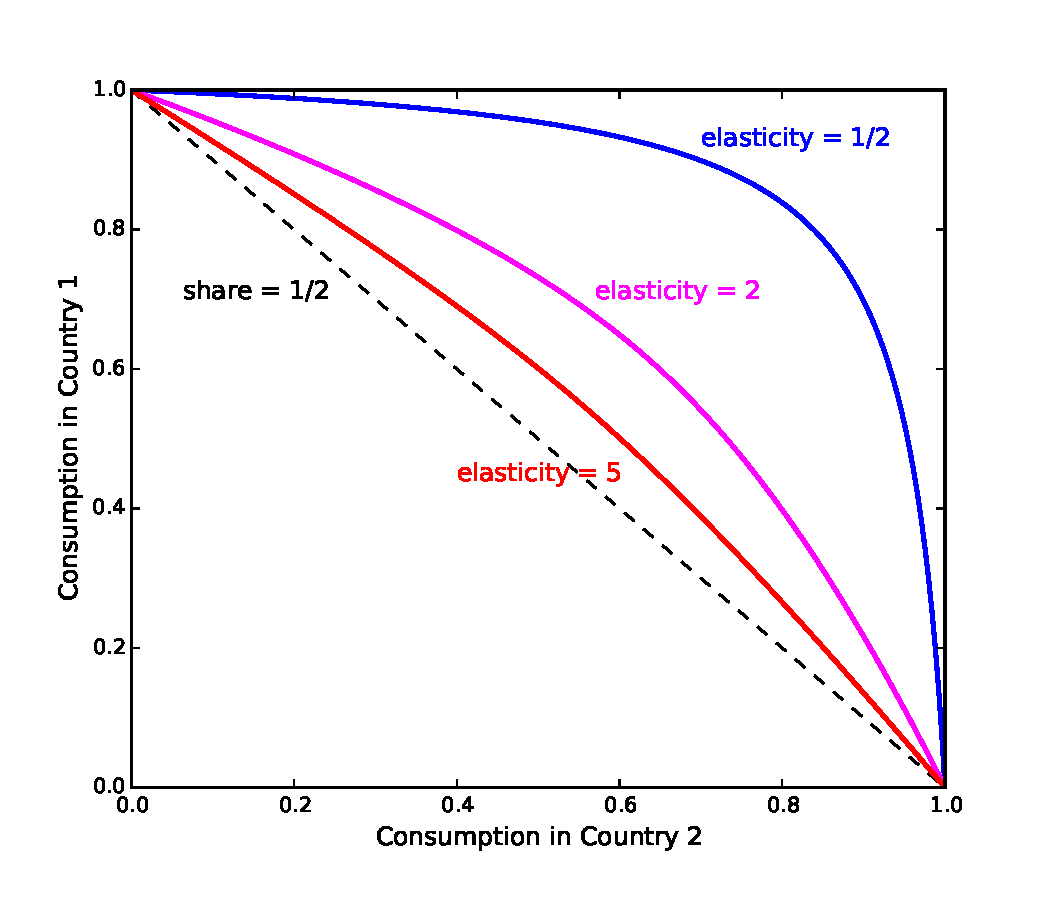
\includegraphics[width=\textwidth]{images/BCFL/final-goods-frontier.pdf}
\label{fig:consumption-frontier}
\end{figure}


% ****************************************************************************
\clearpage
\begin{figure}[htb]
\caption{Pareto and consumption frontiers.
The outer line is the consumption frontier with benchmark parameter values.
The inner line is the Pareto frontier:  the utility $J$ of agent 1 given
promised utility $U$ to agent 2.
In each case, the other state variables are $z_{1t} = z_{2t} = \wh{z}_t = 1$
and $v_t = v$.}

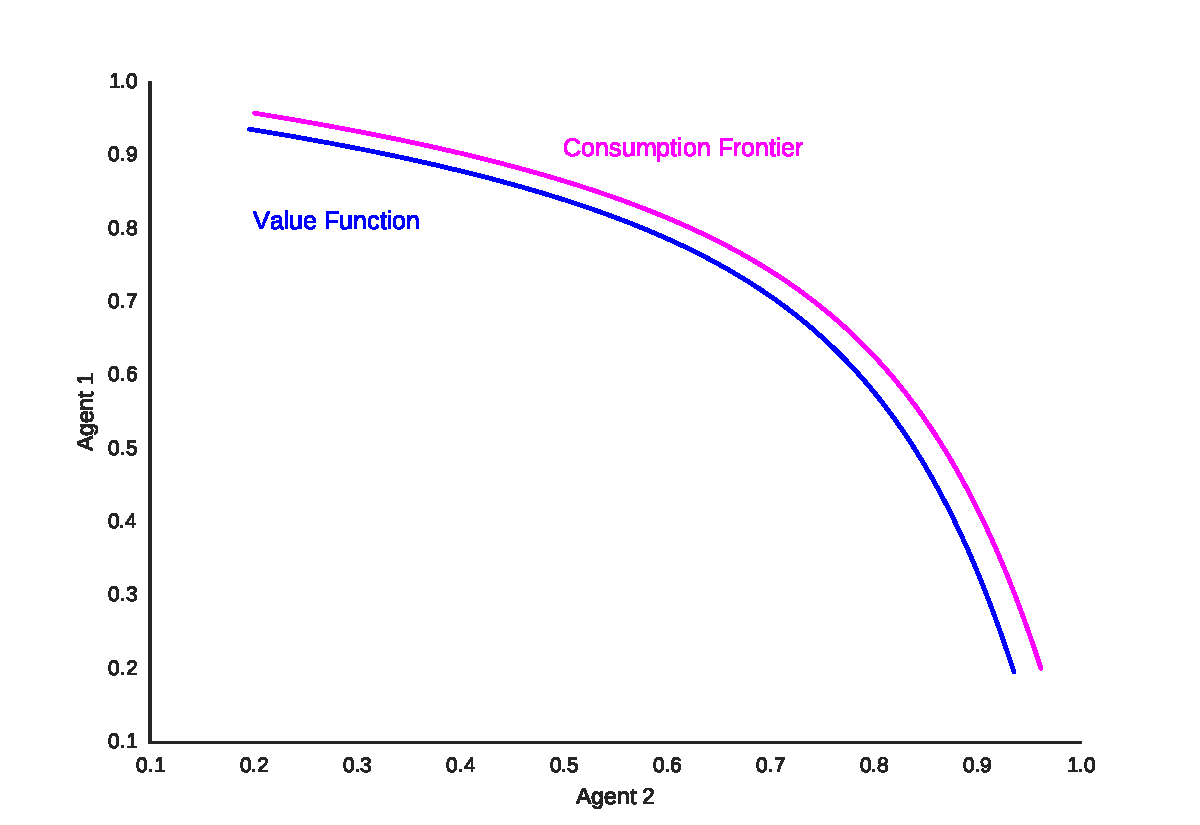
\includegraphics[width=\textwidth]{images/BCFL/frontiers_alpha9.pdf}
\label{fig:pareto-frontier}
\end{figure}


% ****************************************************************************
\clearpage
\begin{figure}[htb]
\caption{Dynamics of the additive and recursive Pareto weight.
The two lines represent simulations of models with additive ($\alpha = \rho = -1$)
and recursive ($\alpha = -9$, $\rho = -1 $) preferences.
The simulations use the same paths for exogenous state variables.
In each case, we plot $\log \lambda_t^*$ against time. }

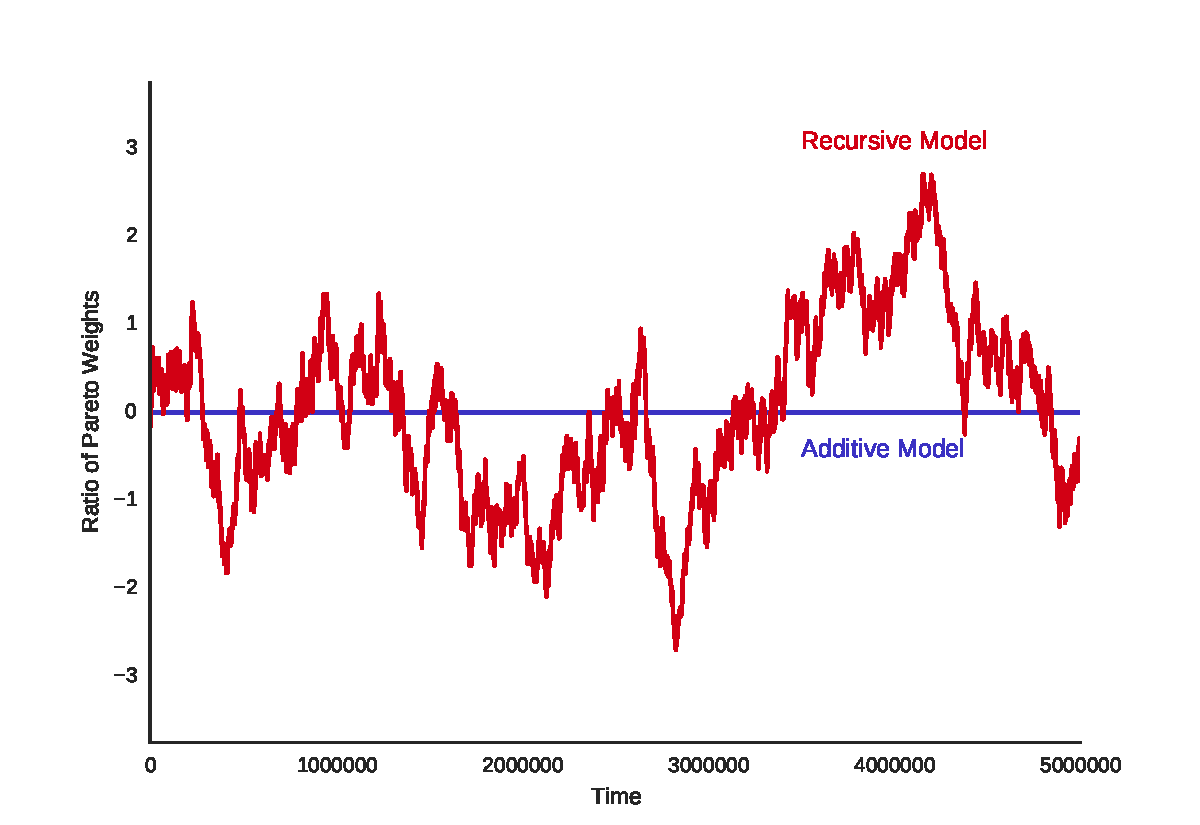
\includegraphics[width=\textwidth]{images/BCFL/paretoweightstability_alpha9.pdf}
\label{fig:exchange-pareto-weight-two}
\end{figure}


% ****************************************************************************
\clearpage
\begin{figure}[htb]
\caption{Risk aversion and expected changes in the Pareto weight.
The lines represent the expected change in $\log \lambda_t^*$, or $E_t[\log \lambda^*_{t+1}] - \log \lambda_t$,
with three values of risk aversion $1-\alpha$:
$2$ (additive), 10, and 50. }

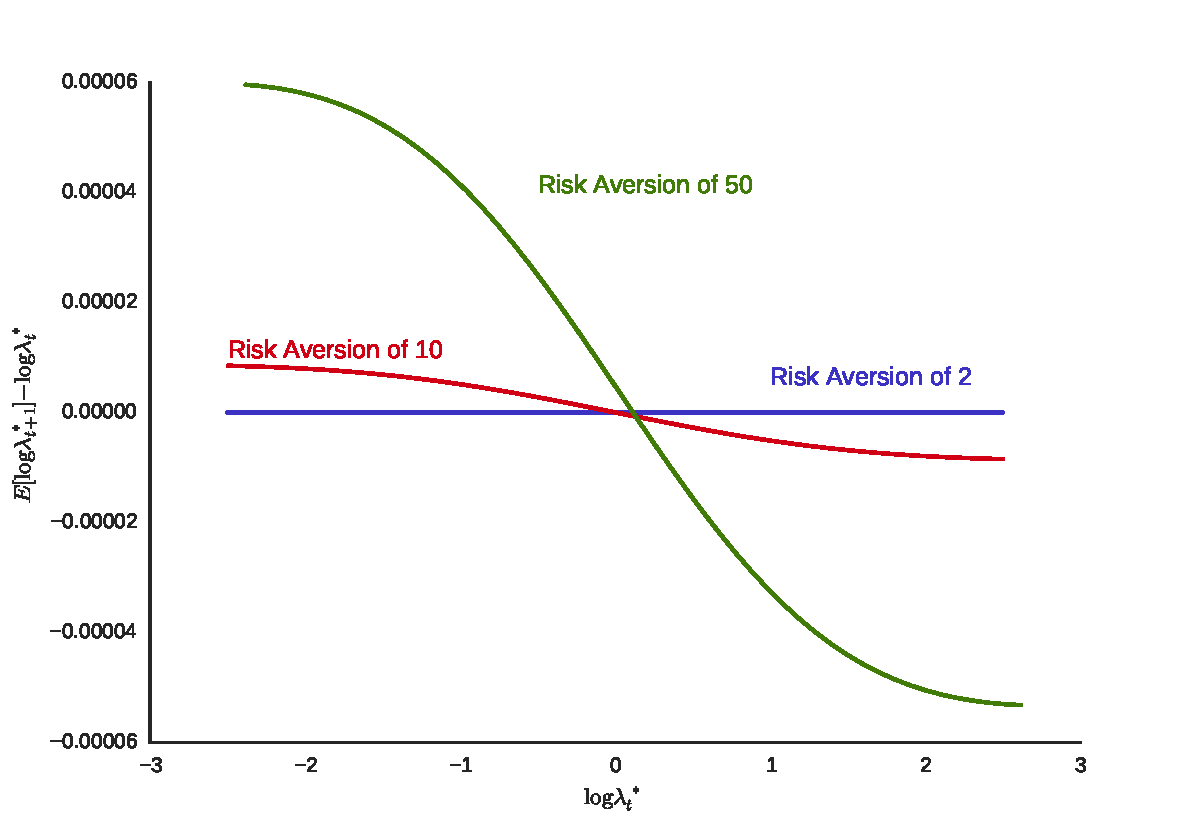
\includegraphics[width=\textwidth]{images/BCFL/policy_at_ss_one_axis.pdf}
\label{fig:change-pareto-weight-ra}
\end{figure}


% ****************************************************************************
\clearpage
\begin{figure}[htb]
\caption{Armington substitutability and expected changes in the Pareto weight.
The lines represent the expected change in $\log \lambda_t^*$, or $E_t[\log \lambda^*_{t+1}] - \log \lambda_t$,
with three values of the substitutability parameter $\sigma$ in the Armington aggregator.
The elasticities $1/(1-\sigma)$ are 2/3, 1, and 2. }

\bigskip
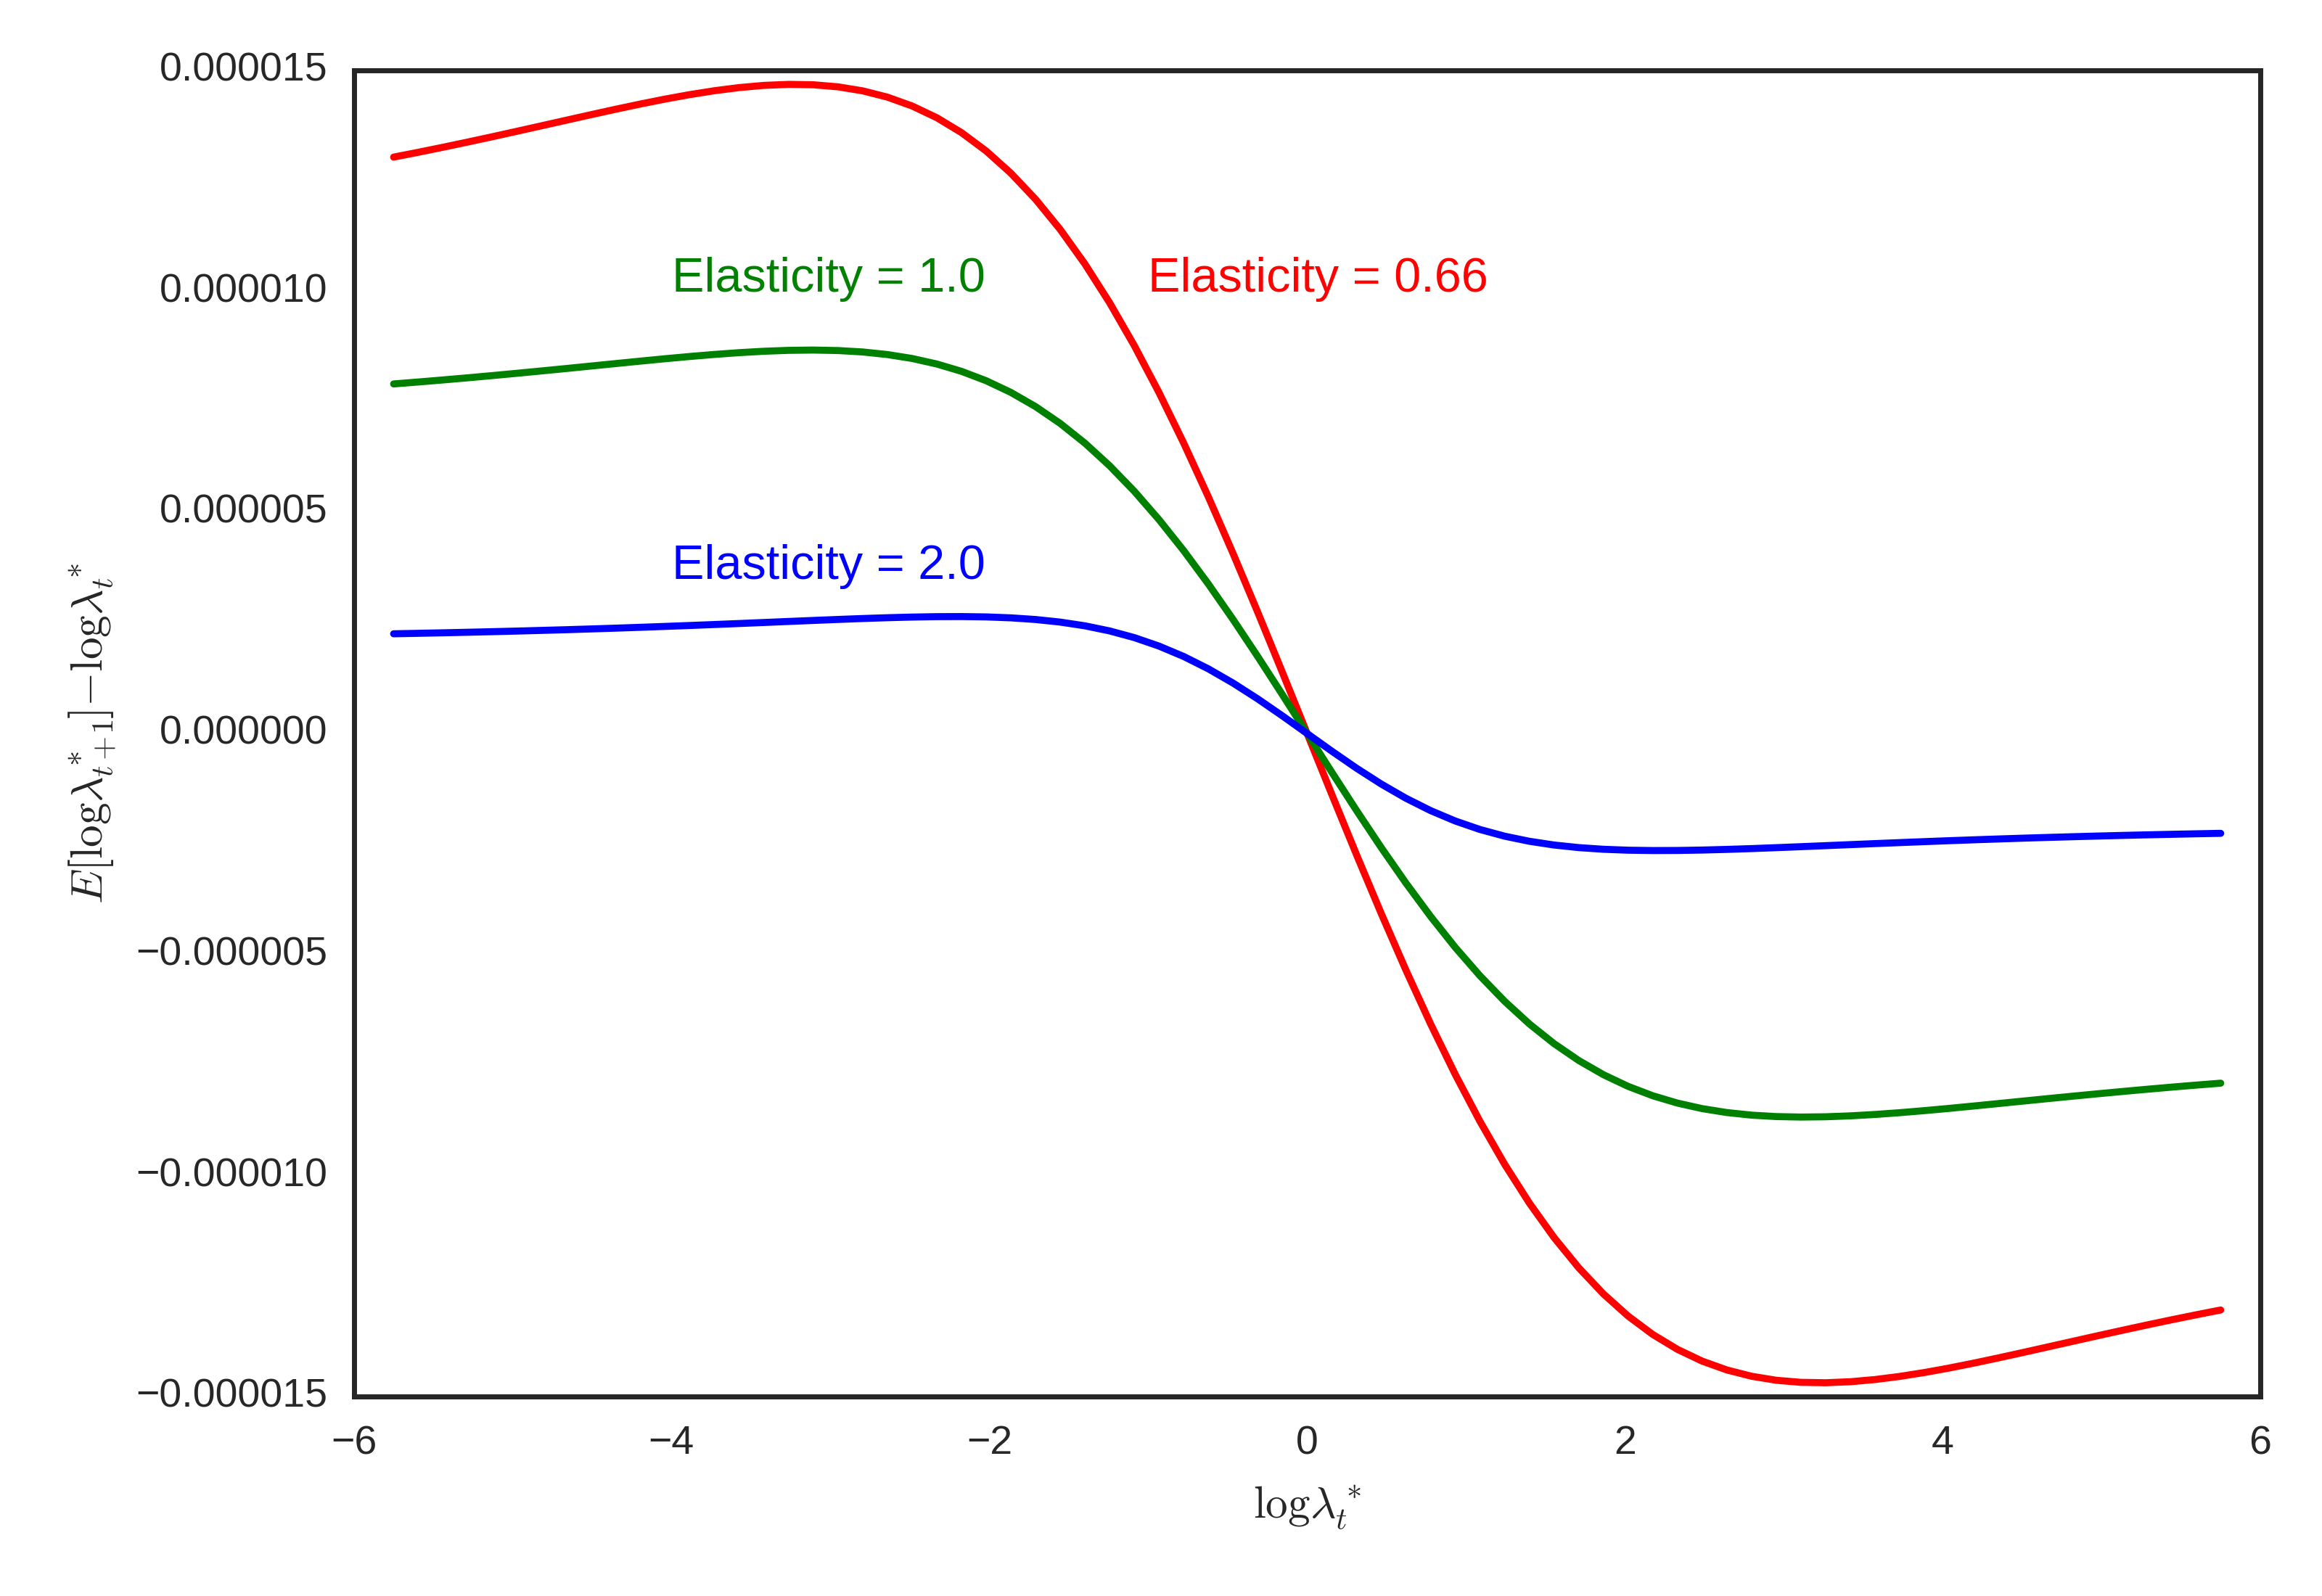
\includegraphics[width=\textwidth]{images/BCFL/Policies_Diff_Elast.png}
\label{fig:change-pareto-weight-arm}
\end{figure}

% ****************************************************************************
\clearpage
\begin{figure}[htb]
\caption{Intertemporal substitution and expected changes in the Pareto weight.
The lines represent the expected change in $\log \lambda_t^*$, or $E_t[\log \lambda^*_{t+1}] - \log \lambda_t$,
with three values of the substitutability parameter $\rho$ in the time aggregator:
$-1$, $-0.01$, and 1/3.
They correspond to intertemporal elasticities of substitution of 1/2, 0.99, and 3/2. }

\bigskip
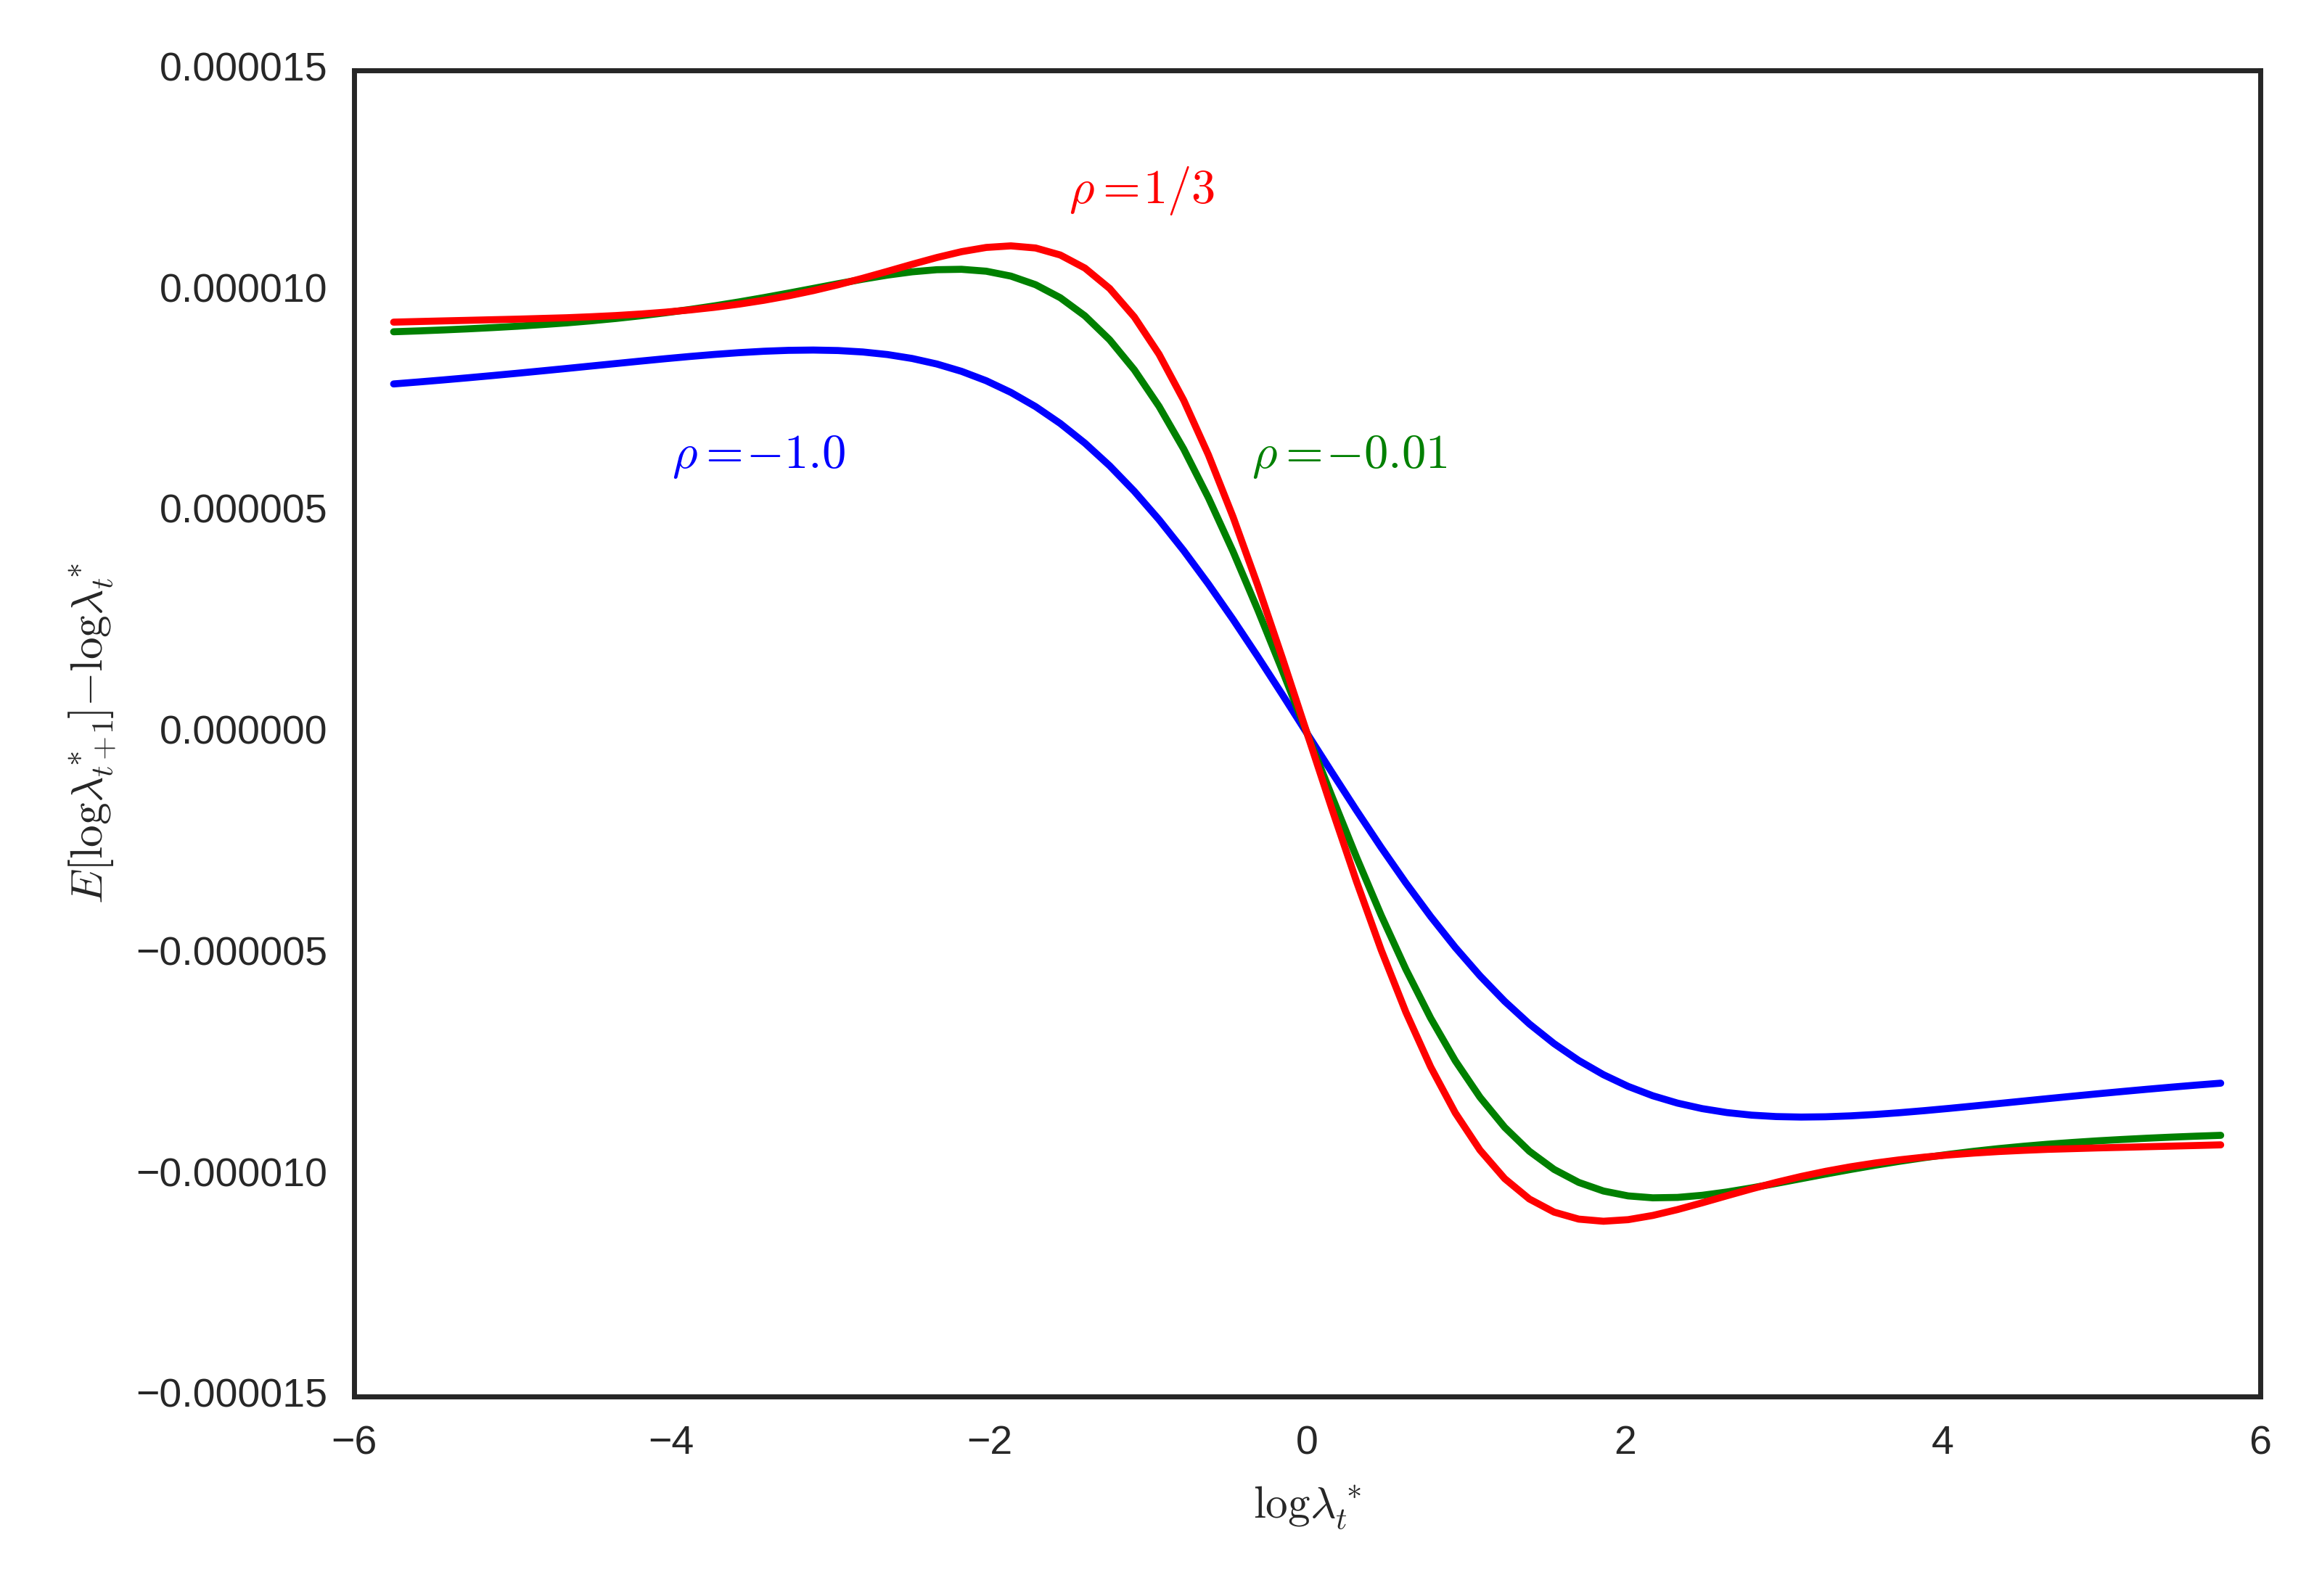
\includegraphics[width=\textwidth]{images/BCFL/Policies_Diff_rho.png}
\label{fig:change-pareto-weight-ies}
\end{figure}


% ****************************************************************************
\clearpage
\begin{figure}[htb]
\caption{Consumption and the real exchange rate.
The dots represent simulations of models with additive ($\alpha = \rho = -1$)
and recursive ($\alpha = -9$) preferences.
In each case, we plot  $\log e_t = \log (p_{2t}/p_{1t}) $ against $\log (c_{2t}/c_{1t}) $
for a simulation of the model. }

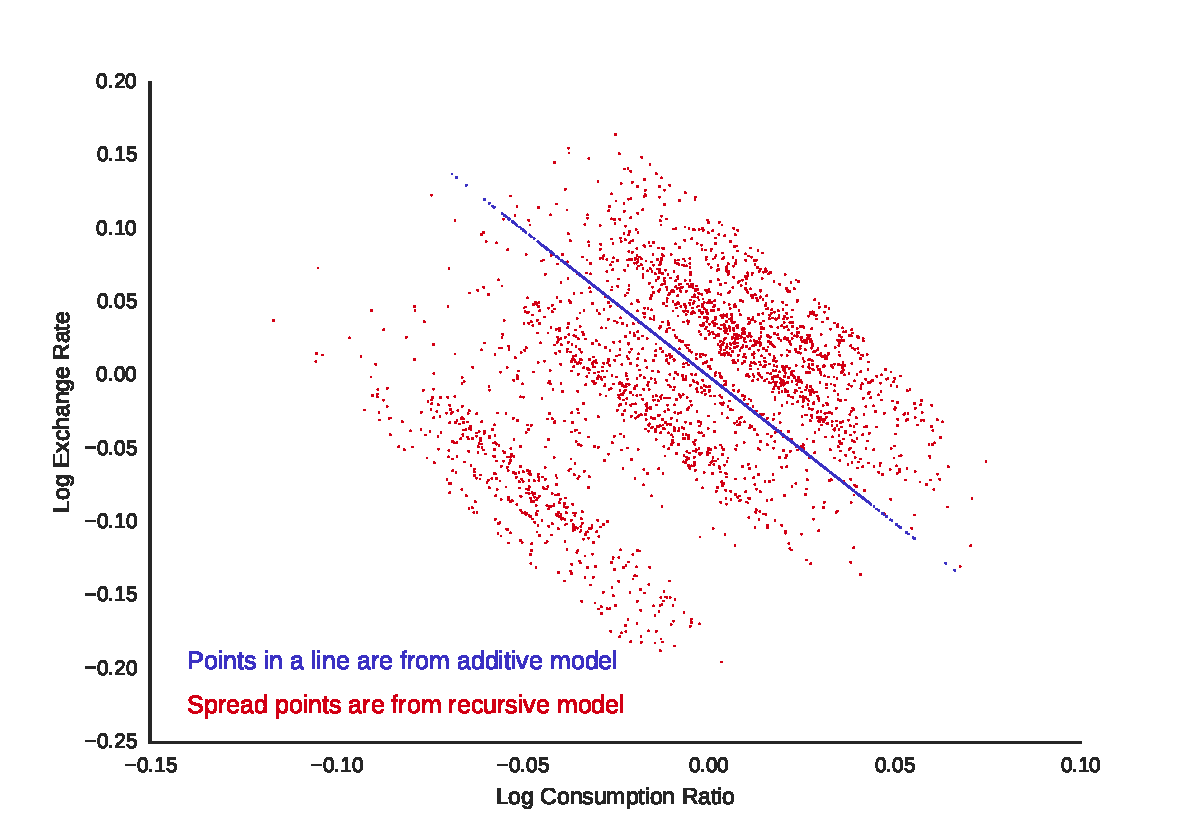
\includegraphics[width=\textwidth]{images/BCFL/con_v_fxr_alpha9.pdf}
\label{fig:exchange-cons-rer-two}
\end{figure}

%\end{document}
% ****************************************************************************
\clearpage
\begin{figure}[htb]
\caption{Dynamics of the real exchange rate.
The lines represent autocorrelation functions for the real exchange rate
($\log e_t$) in models with additive ($\alpha = \rho = -1$)
and recursive ($\alpha = -9$) preferences.}

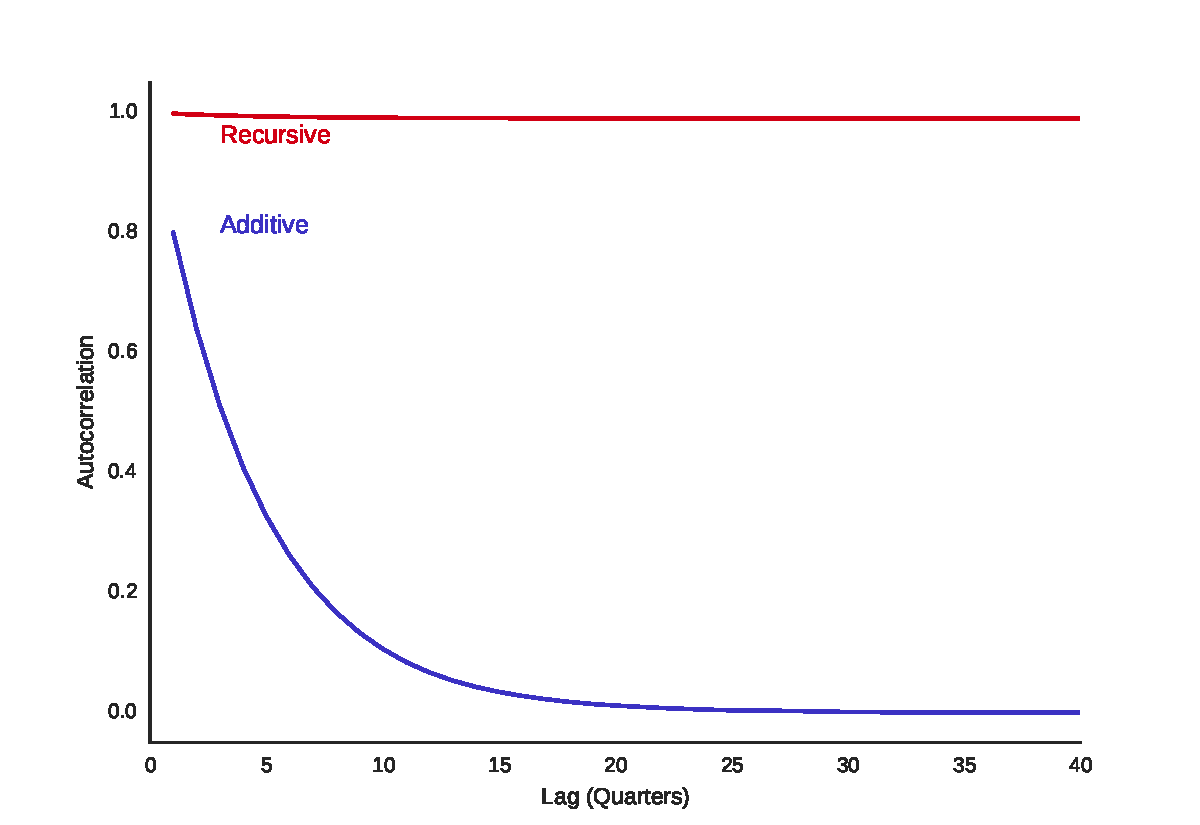
\includegraphics[width=\textwidth]{images/BCFL/acorr_fx_alpha1_9_one_axis.pdf}
\label{fig:rer-acfs}
\end{figure}

%\end{document}
% ****************************************************************************
\clearpage
\begin{figure}[htb]
\caption{Responses of variables
to an impulse in relative productivity\newline
$\log \wh{z}_t = (1/2) (\log z_{1t} - \log z_{2t}) $ in country 2.
The impulse takes place at date $t=1$.
Responses are reported as percent deviations from mean values.
}

\bigskip
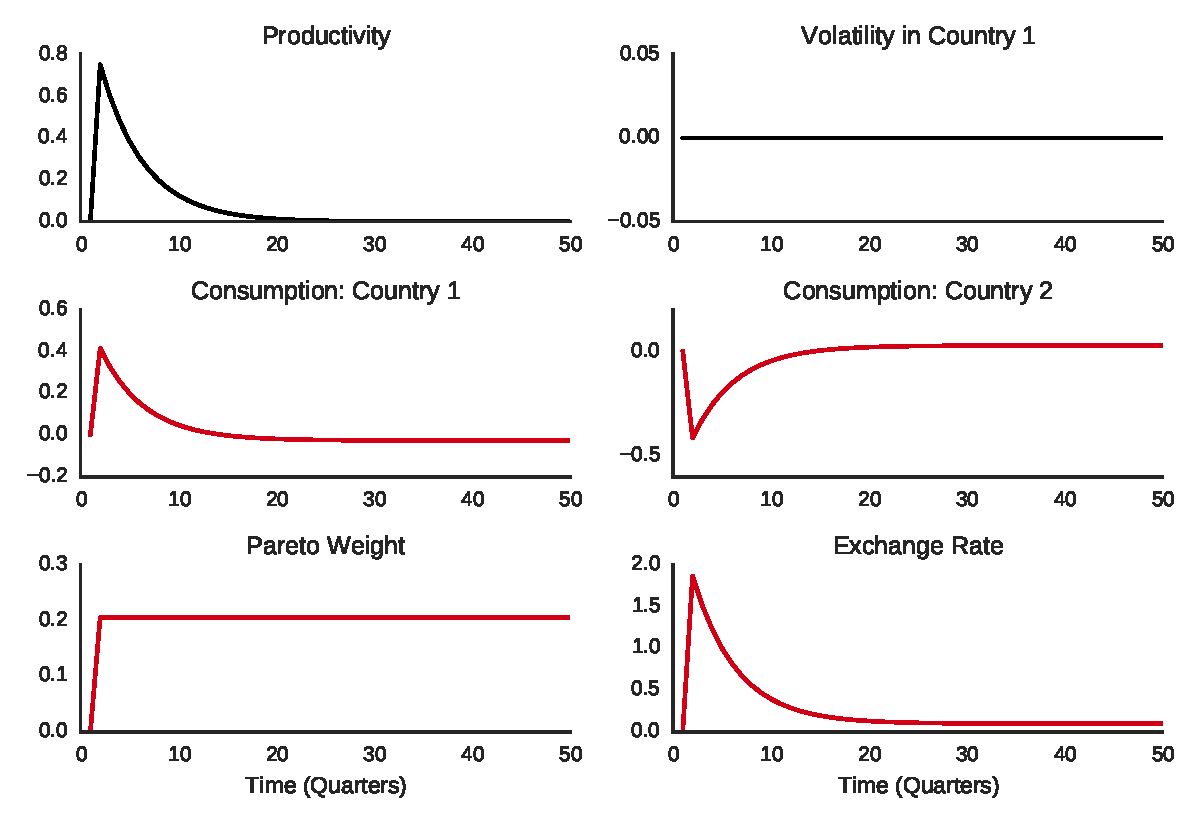
\includegraphics[width=\textwidth]{images/BCFL/irf_wrt_zhat_alpha9.pdf}
\label{fig:irf-zhat}
\end{figure}

%\end{document}
% ****************************************************************************
\clearpage
\begin{figure}[htb]
\caption{Responses of variables
to an impulse in volatility $v_t$.
The impulse takes place at date $t=1$.
Responses are reported as percent deviations from mean values.
}

\bigskip
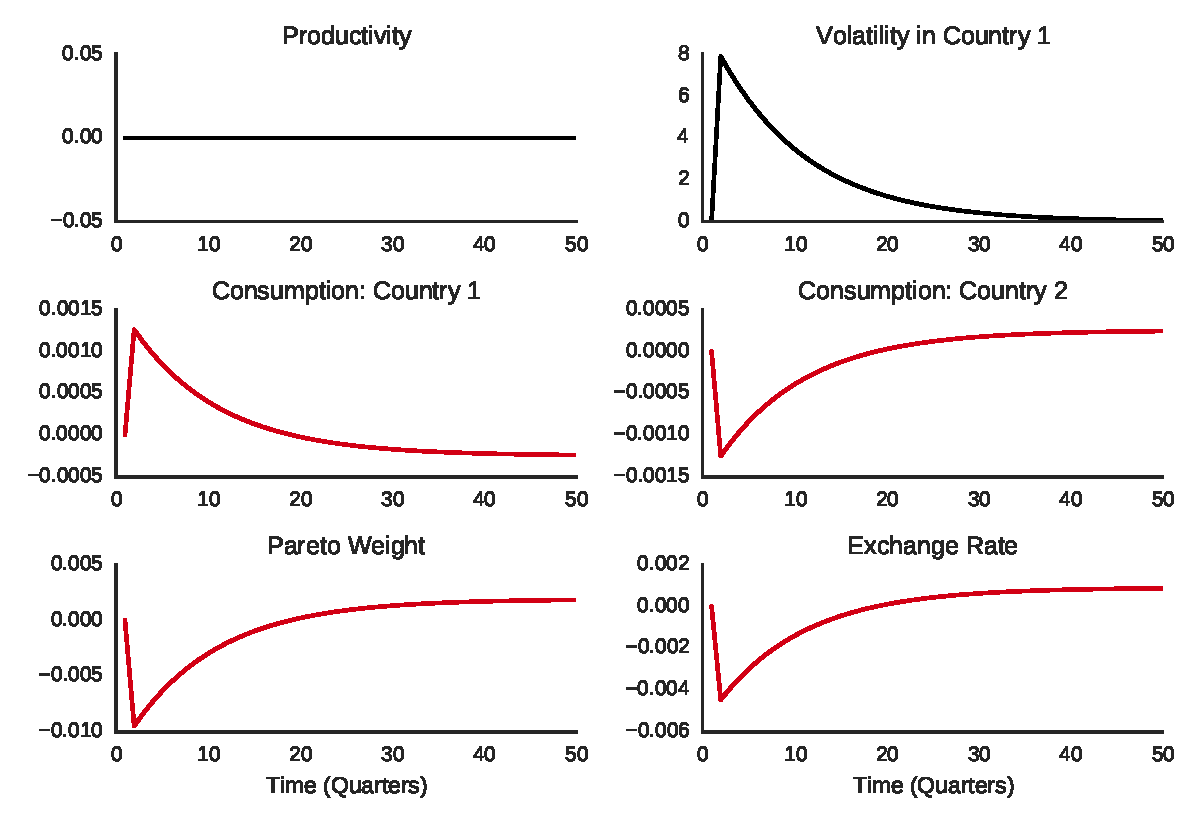
\includegraphics[width=\textwidth]{images/BCFL/irf_wrt_v_alpha9.pdf}
\label{fig:irf-v}
\end{figure}


% APPENDIX 2
\chapter{Supplementary Material for Chapter 2} \label{sec:Appendix2}

  %!TEX root = ../../dissertation.tex

\section{Data} \label{sec:data_appendix}

  Due to the sensitive nature of information on an individual's education data, one difficulty of
  any empirical work on higher education financing is the scarcity of publically available micro
  data. In conclusion to a discussion of how an economist might design a student loans program,
  \cite{Dynarski2014} claims, ``Designing such a program requires detailed data on individual
  earnings and borrowing, which are currently unavailable to researchers within and outside the
  government. If loan policy is to be firmly grounded in research, this gap in the data must be
  closed.'' While not as accurate as administrative data, we leverage several data sets on education
  and earnings outcomes in this paper.

  \textbf{High School and Beyond}: The High School and Beyond survey is a longitudinal survey that
  follows individuals who were either sophmores or seniors in 1980 through 1992\footnote{The
  individuals who were high school sophmores in 1980 were interviewed in 1980, 1982, 1984, 1986, and
  1992 while the individuals who were high school seniors were only interviewed in 1980, 1982, 1984,
  and 1986}. We did not have access to the restricted access micro data and associated transcript
  data, but \cite{HendricksLeukhina2017}, who did have access, published many relevant moments from
  this data set. We take advantage of this and use their empirical estimates for various parameters
  in our model.

  \textbf{Panel Study of Income Dynamics}: The Panel Study of Income Dynamics (PSID) is the longest
  running longitudinal survey in the world. As in \cite{CarrollSamwick1997}, \cite{Guvenen2009}, and
  \cite{Hryshko2012} the PSID will be used to estimate income dynamics --- We successfully replicate
  estimated income processes from these papers and will use them as inputs to our model.

  %!TEX root = ../../dissertation.tex

\section{Tables and Figures}

\begin{table}
\caption{Benchmark parameter values.}
\tabcolsep=0.2in
\centering
\begin{tabular}{lrl}
\toprule
Parameter  &  Value  &  Comment \\
\midrule

%& \\
\multicolumn{3}{l}{\textit Preferences} \\
$\rho$   &  $-1$  & IES $= 1/(1-\rho) = 1/2$ \\
$\alpha$ &  $-9$ & RA $= 1-\alpha = 10$ \\ %, Bansal \& Yaron (2004, Table II) \\
$\beta$  &   0.98 &  \\

\multicolumn{3}{l}{\textit Armington aggregator}  \\
$\sigma$    &   0   &  Cobb-Douglas   \\
$\omega$    &  0.1  &  chosen to hit import share of 0.1  \\

\multicolumn{3}{l}{\textit Productivity growth  } \\
$\log g$  &  0.004   &  Tallarini (2000, Table 4) \\
$v^{1/2}$ & 0.015   &  Tallarini (2000, Table 4), rounded off \\
$ \varphi_v$ & 0.95 & Backus, Ferriere, and Zin (2015, Table 1) \\
$ \tau$   &  $0.74 \times 10^{-5}$  & makes $v$ three standard deviations from zero \\
$ \gamma$ & 0.1 & persistence of productivity difference \\
\bottomrule
\end{tabular}
\label{tab:benchmark}
\end{table}



% ****************************************************************************
\clearpage
\begin{figure}[htb]
\caption{Consumption frontiers.
Lines represent the frontier quantities of consumption given unit quantities of the intermediate goods.
The dashed black line has $\omega = 1/2$, making the two final goods the same.
For the others, we choose an import share of 0.1
and use (\ref{eq:share-calculation}) to adjust $\omega$ as we vary $\sigma$.
The elasticities of substitution noted in the figure are $1/(1-\sigma)$.}

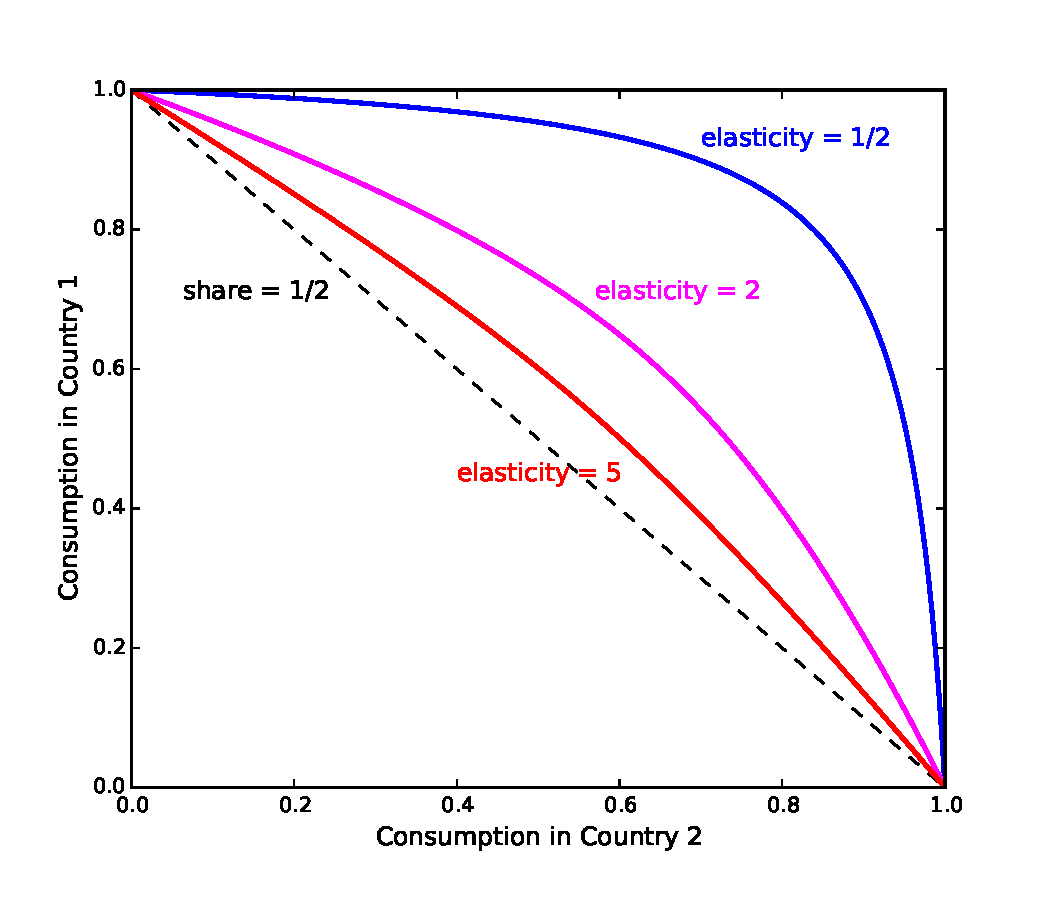
\includegraphics[width=\textwidth]{images/BCFL/final-goods-frontier.pdf}
\label{fig:consumption-frontier}
\end{figure}


% ****************************************************************************
\clearpage
\begin{figure}[htb]
\caption{Pareto and consumption frontiers.
The outer line is the consumption frontier with benchmark parameter values.
The inner line is the Pareto frontier:  the utility $J$ of agent 1 given
promised utility $U$ to agent 2.
In each case, the other state variables are $z_{1t} = z_{2t} = \wh{z}_t = 1$
and $v_t = v$.}

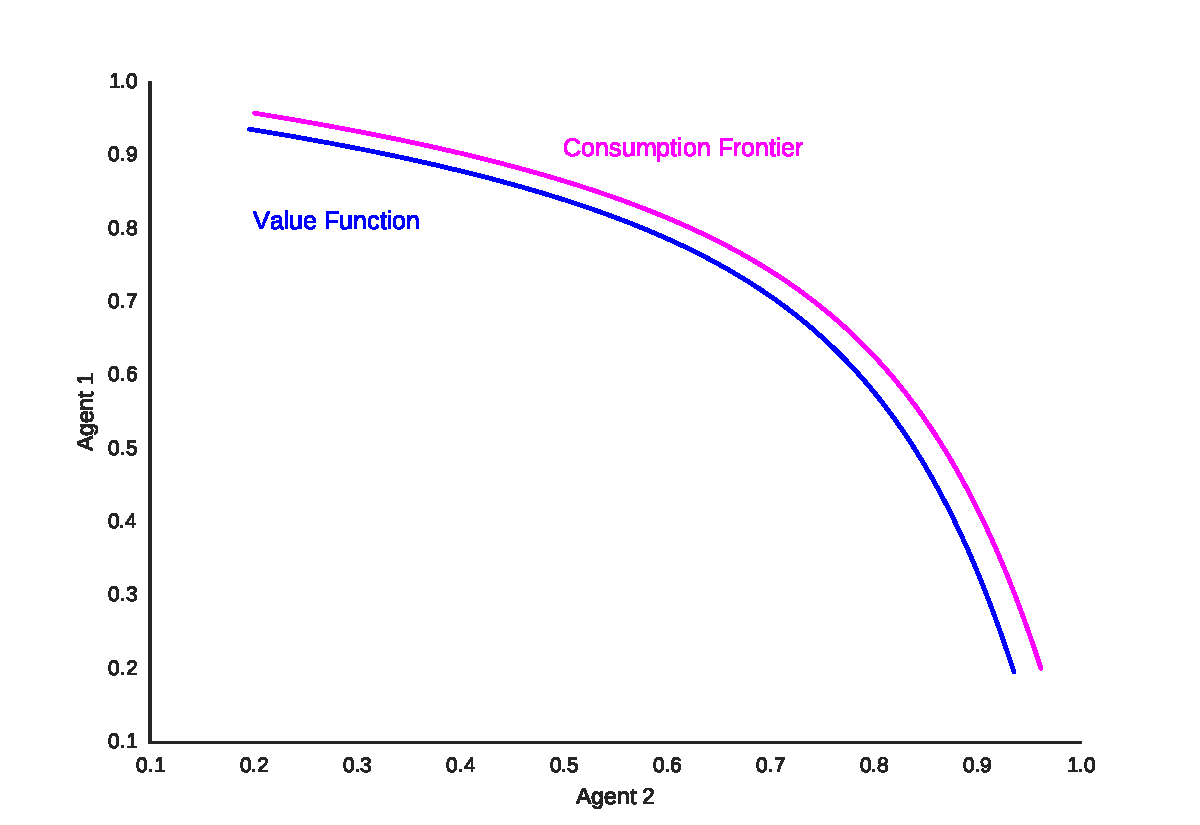
\includegraphics[width=\textwidth]{images/BCFL/frontiers_alpha9.pdf}
\label{fig:pareto-frontier}
\end{figure}


% ****************************************************************************
\clearpage
\begin{figure}[htb]
\caption{Dynamics of the additive and recursive Pareto weight.
The two lines represent simulations of models with additive ($\alpha = \rho = -1$)
and recursive ($\alpha = -9$, $\rho = -1 $) preferences.
The simulations use the same paths for exogenous state variables.
In each case, we plot $\log \lambda_t^*$ against time. }

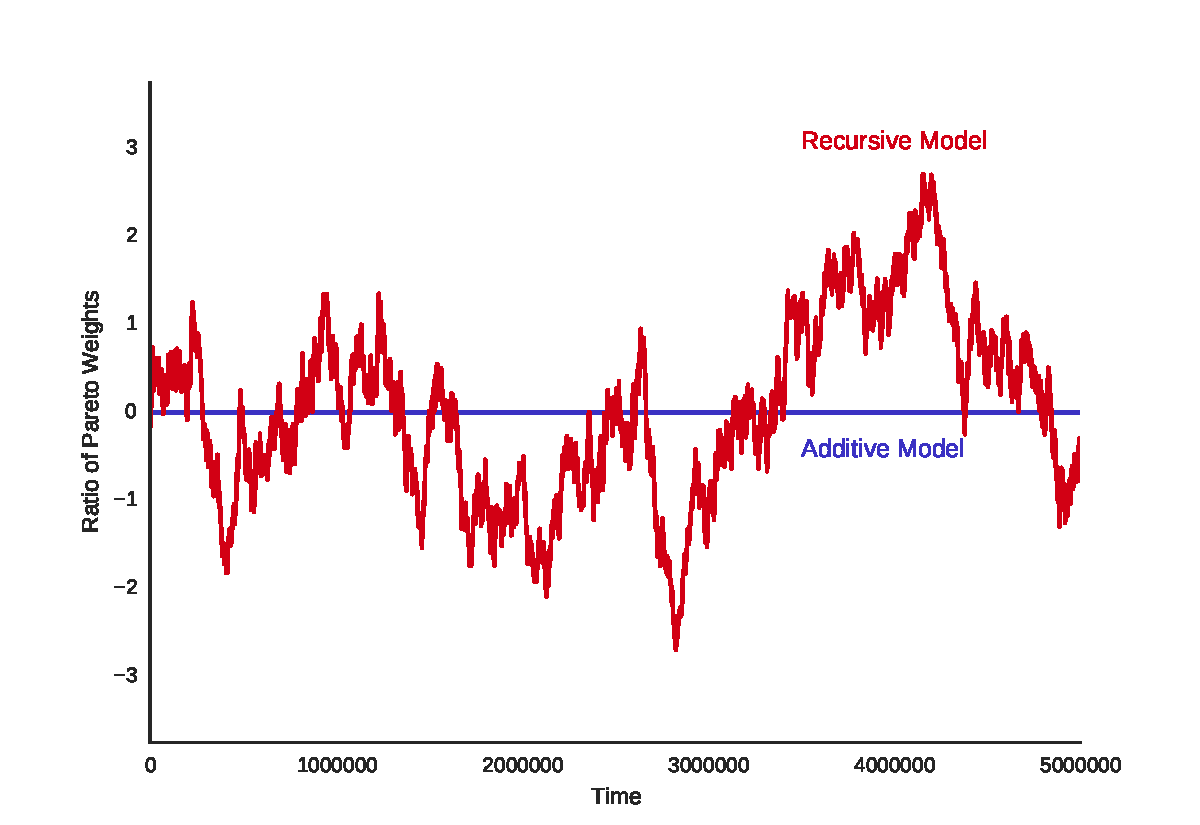
\includegraphics[width=\textwidth]{images/BCFL/paretoweightstability_alpha9.pdf}
\label{fig:exchange-pareto-weight-two}
\end{figure}


% ****************************************************************************
\clearpage
\begin{figure}[htb]
\caption{Risk aversion and expected changes in the Pareto weight.
The lines represent the expected change in $\log \lambda_t^*$, or $E_t[\log \lambda^*_{t+1}] - \log \lambda_t$,
with three values of risk aversion $1-\alpha$:
$2$ (additive), 10, and 50. }

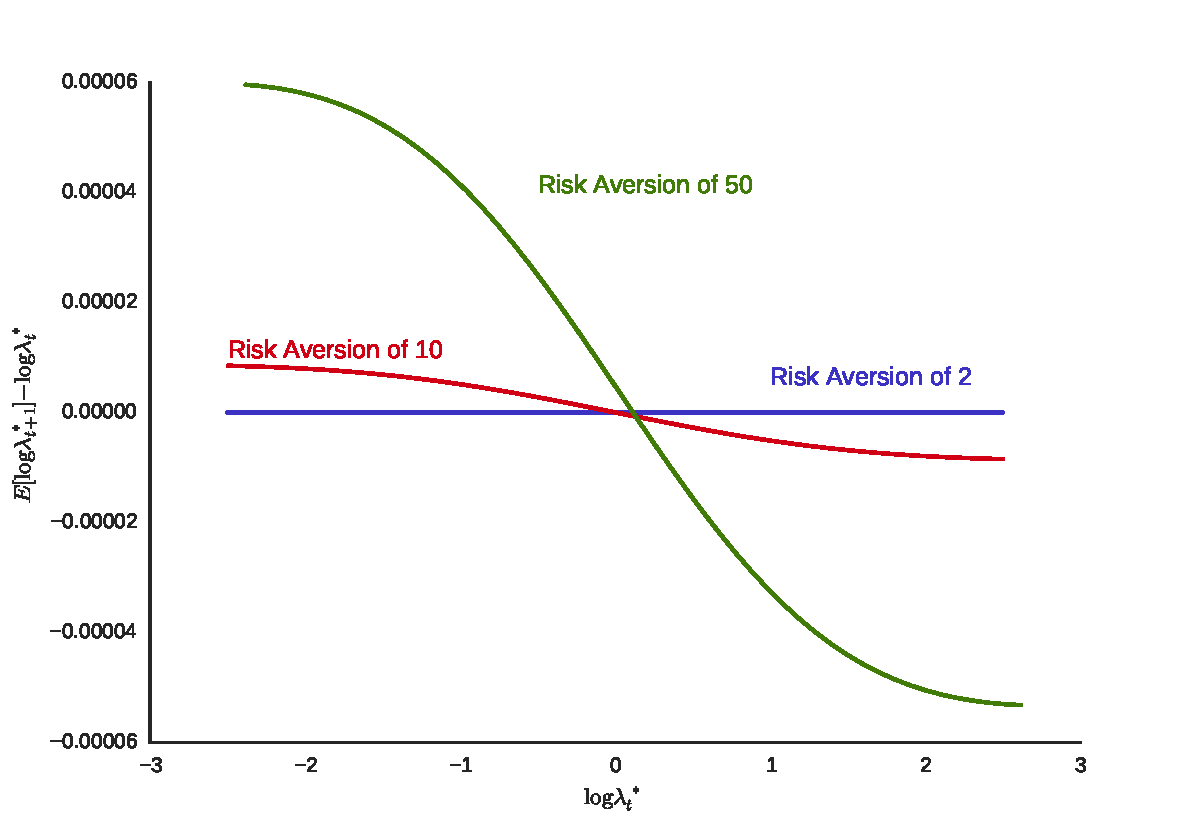
\includegraphics[width=\textwidth]{images/BCFL/policy_at_ss_one_axis.pdf}
\label{fig:change-pareto-weight-ra}
\end{figure}


% ****************************************************************************
\clearpage
\begin{figure}[htb]
\caption{Armington substitutability and expected changes in the Pareto weight.
The lines represent the expected change in $\log \lambda_t^*$, or $E_t[\log \lambda^*_{t+1}] - \log \lambda_t$,
with three values of the substitutability parameter $\sigma$ in the Armington aggregator.
The elasticities $1/(1-\sigma)$ are 2/3, 1, and 2. }

\bigskip
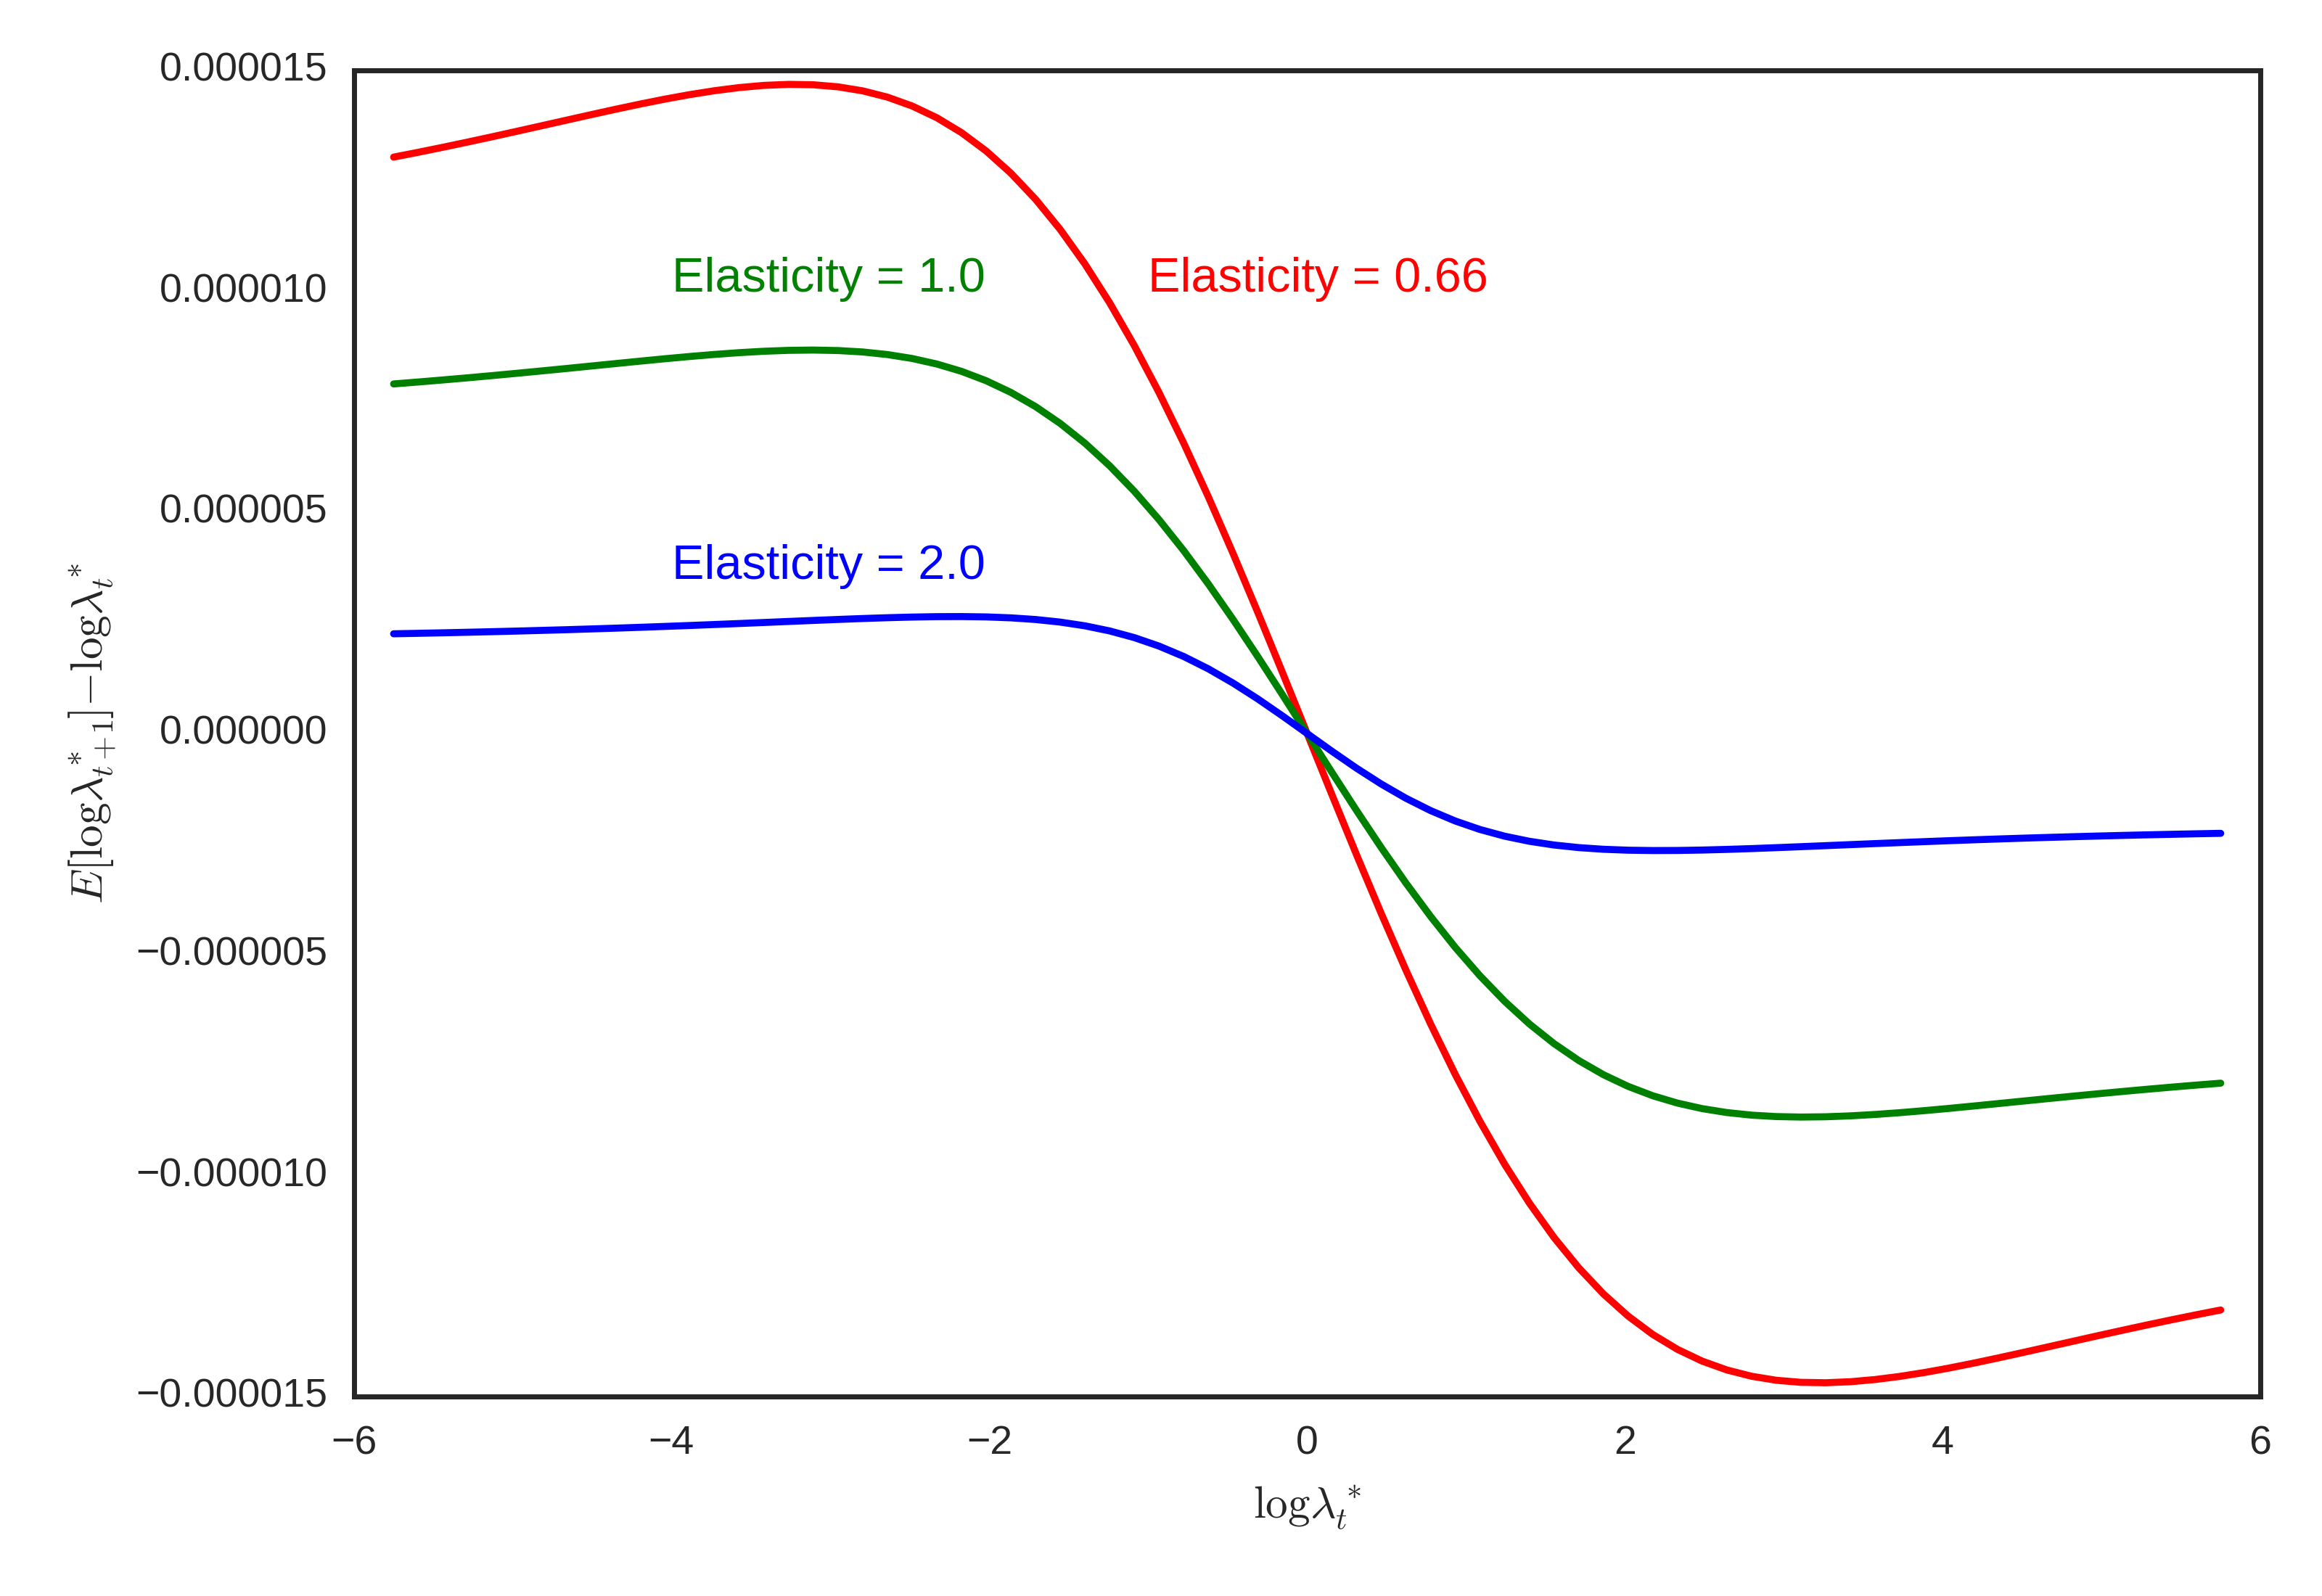
\includegraphics[width=\textwidth]{images/BCFL/Policies_Diff_Elast.png}
\label{fig:change-pareto-weight-arm}
\end{figure}

% ****************************************************************************
\clearpage
\begin{figure}[htb]
\caption{Intertemporal substitution and expected changes in the Pareto weight.
The lines represent the expected change in $\log \lambda_t^*$, or $E_t[\log \lambda^*_{t+1}] - \log \lambda_t$,
with three values of the substitutability parameter $\rho$ in the time aggregator:
$-1$, $-0.01$, and 1/3.
They correspond to intertemporal elasticities of substitution of 1/2, 0.99, and 3/2. }

\bigskip
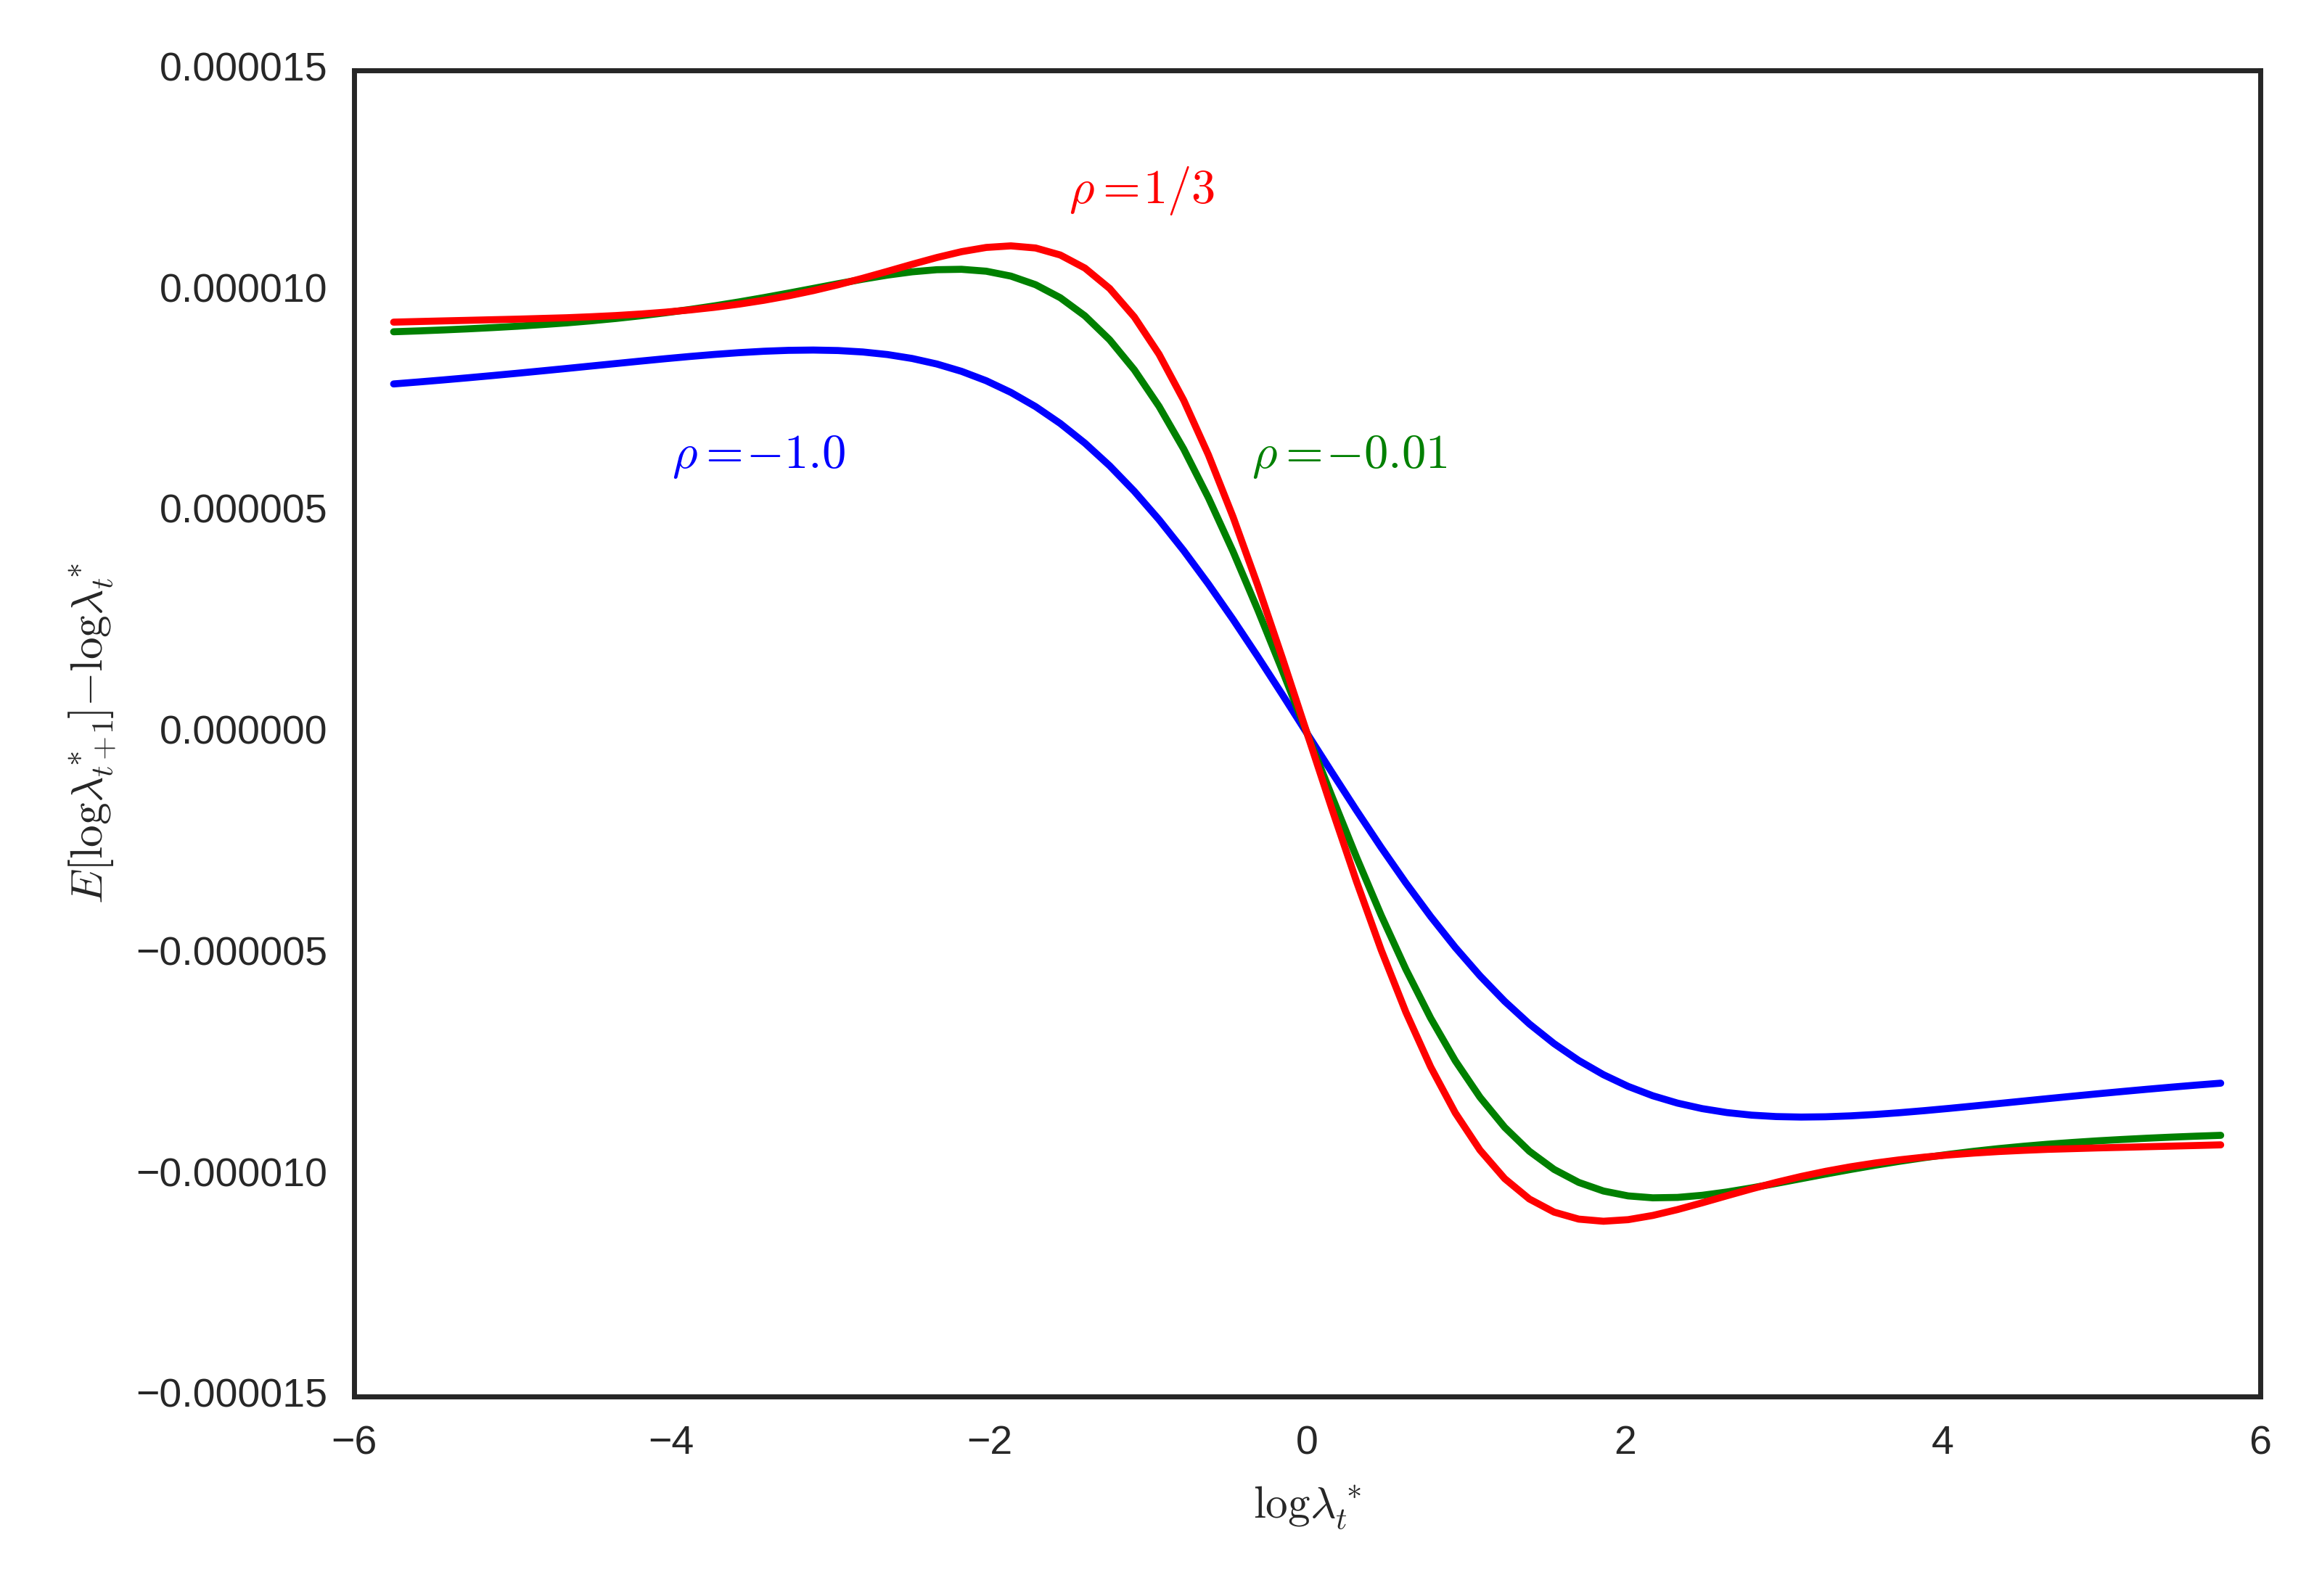
\includegraphics[width=\textwidth]{images/BCFL/Policies_Diff_rho.png}
\label{fig:change-pareto-weight-ies}
\end{figure}


% ****************************************************************************
\clearpage
\begin{figure}[htb]
\caption{Consumption and the real exchange rate.
The dots represent simulations of models with additive ($\alpha = \rho = -1$)
and recursive ($\alpha = -9$) preferences.
In each case, we plot  $\log e_t = \log (p_{2t}/p_{1t}) $ against $\log (c_{2t}/c_{1t}) $
for a simulation of the model. }

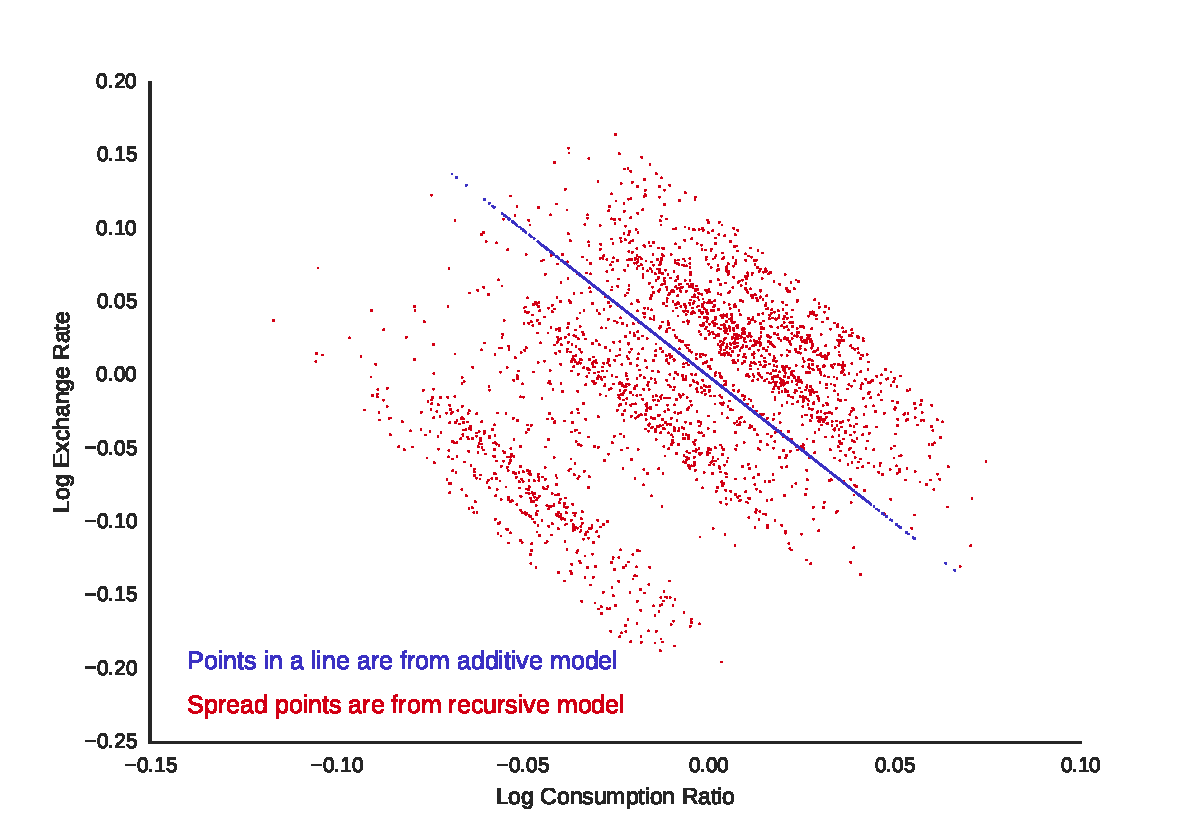
\includegraphics[width=\textwidth]{images/BCFL/con_v_fxr_alpha9.pdf}
\label{fig:exchange-cons-rer-two}
\end{figure}

%\end{document}
% ****************************************************************************
\clearpage
\begin{figure}[htb]
\caption{Dynamics of the real exchange rate.
The lines represent autocorrelation functions for the real exchange rate
($\log e_t$) in models with additive ($\alpha = \rho = -1$)
and recursive ($\alpha = -9$) preferences.}

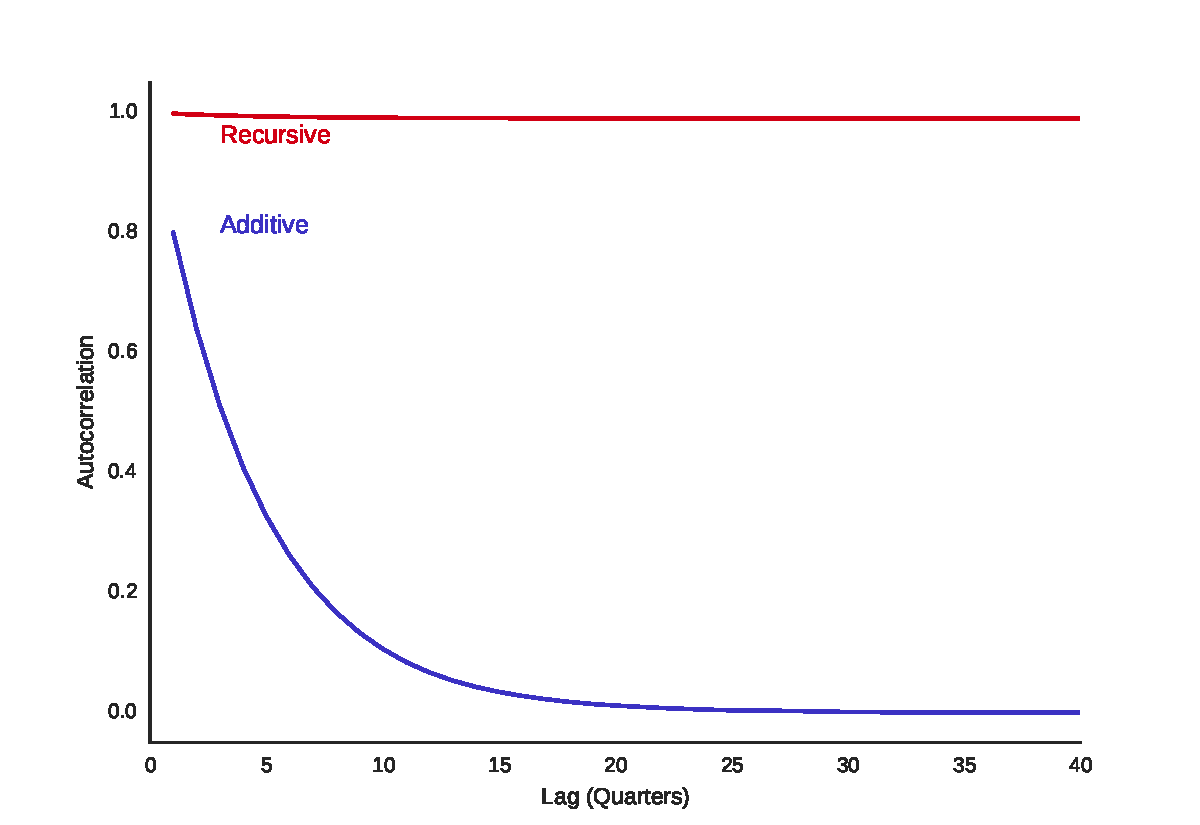
\includegraphics[width=\textwidth]{images/BCFL/acorr_fx_alpha1_9_one_axis.pdf}
\label{fig:rer-acfs}
\end{figure}

%\end{document}
% ****************************************************************************
\clearpage
\begin{figure}[htb]
\caption{Responses of variables
to an impulse in relative productivity\newline
$\log \wh{z}_t = (1/2) (\log z_{1t} - \log z_{2t}) $ in country 2.
The impulse takes place at date $t=1$.
Responses are reported as percent deviations from mean values.
}

\bigskip
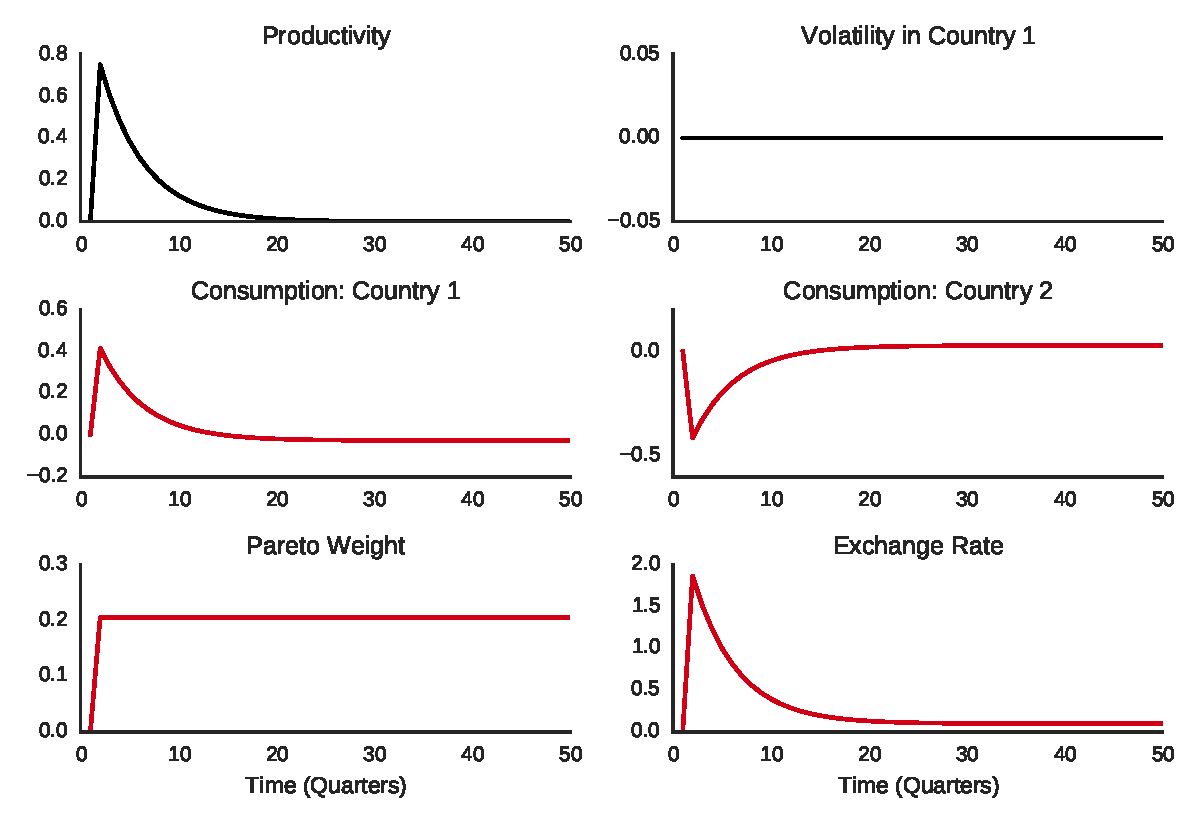
\includegraphics[width=\textwidth]{images/BCFL/irf_wrt_zhat_alpha9.pdf}
\label{fig:irf-zhat}
\end{figure}

%\end{document}
% ****************************************************************************
\clearpage
\begin{figure}[htb]
\caption{Responses of variables
to an impulse in volatility $v_t$.
The impulse takes place at date $t=1$.
Responses are reported as percent deviations from mean values.
}

\bigskip
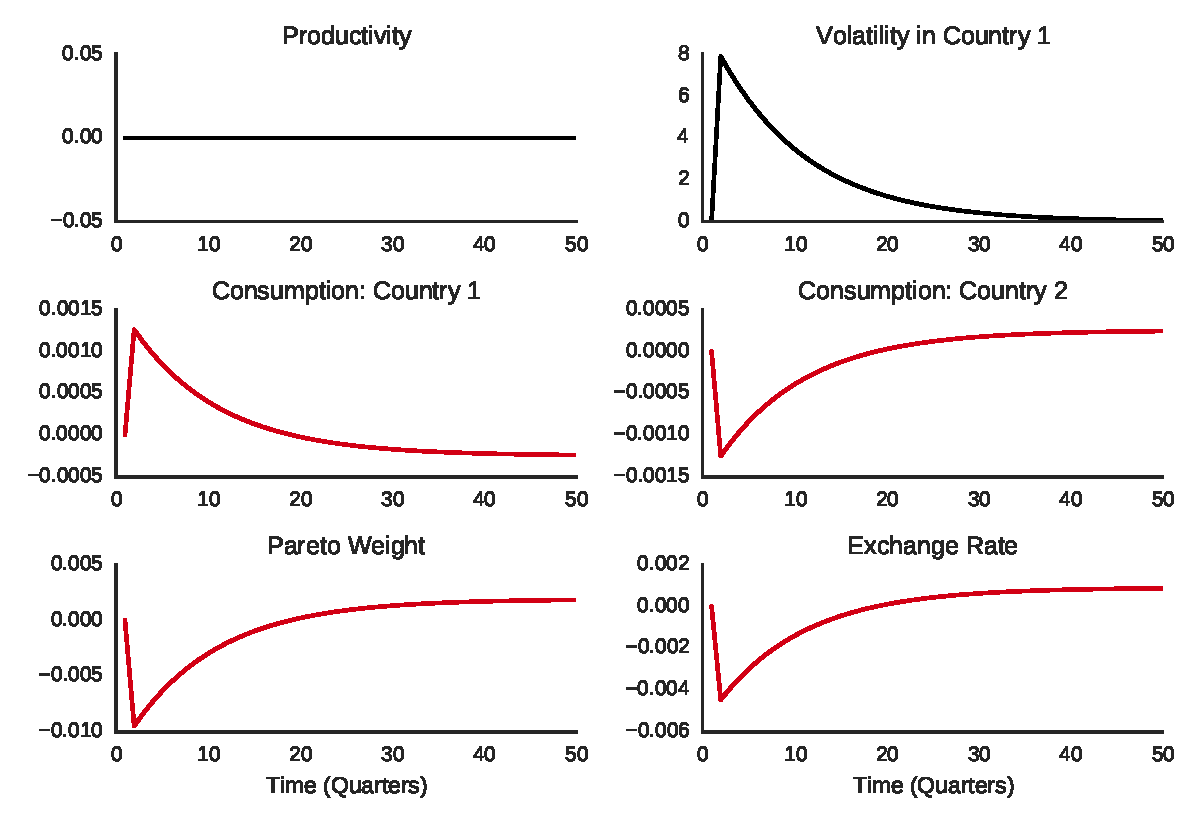
\includegraphics[width=\textwidth]{images/BCFL/irf_wrt_v_alpha9.pdf}
\label{fig:irf-v}
\end{figure}


\newpage
\clearpage

% APPENDIX 3
\chapter{Supplementary Material for Chapter 3} \label{sec:Appendix3}

  %!TEX root = ../../dissertation.tex

\section{Data} \label{sec:data_appendix}

  Due to the sensitive nature of information on an individual's education data, one difficulty of
  any empirical work on higher education financing is the scarcity of publically available micro
  data. In conclusion to a discussion of how an economist might design a student loans program,
  \cite{Dynarski2014} claims, ``Designing such a program requires detailed data on individual
  earnings and borrowing, which are currently unavailable to researchers within and outside the
  government. If loan policy is to be firmly grounded in research, this gap in the data must be
  closed.'' While not as accurate as administrative data, we leverage several data sets on education
  and earnings outcomes in this paper.

  \textbf{High School and Beyond}: The High School and Beyond survey is a longitudinal survey that
  follows individuals who were either sophmores or seniors in 1980 through 1992\footnote{The
  individuals who were high school sophmores in 1980 were interviewed in 1980, 1982, 1984, 1986, and
  1992 while the individuals who were high school seniors were only interviewed in 1980, 1982, 1984,
  and 1986}. We did not have access to the restricted access micro data and associated transcript
  data, but \cite{HendricksLeukhina2017}, who did have access, published many relevant moments from
  this data set. We take advantage of this and use their empirical estimates for various parameters
  in our model.

  \textbf{Panel Study of Income Dynamics}: The Panel Study of Income Dynamics (PSID) is the longest
  running longitudinal survey in the world. As in \cite{CarrollSamwick1997}, \cite{Guvenen2009}, and
  \cite{Hryshko2012} the PSID will be used to estimate income dynamics --- We successfully replicate
  estimated income processes from these papers and will use them as inputs to our model.

  %!TEX root = ../../dissertation.tex

\section{Tables and Figures}

\begin{table}
\caption{Benchmark parameter values.}
\tabcolsep=0.2in
\centering
\begin{tabular}{lrl}
\toprule
Parameter  &  Value  &  Comment \\
\midrule

%& \\
\multicolumn{3}{l}{\textit Preferences} \\
$\rho$   &  $-1$  & IES $= 1/(1-\rho) = 1/2$ \\
$\alpha$ &  $-9$ & RA $= 1-\alpha = 10$ \\ %, Bansal \& Yaron (2004, Table II) \\
$\beta$  &   0.98 &  \\

\multicolumn{3}{l}{\textit Armington aggregator}  \\
$\sigma$    &   0   &  Cobb-Douglas   \\
$\omega$    &  0.1  &  chosen to hit import share of 0.1  \\

\multicolumn{3}{l}{\textit Productivity growth  } \\
$\log g$  &  0.004   &  Tallarini (2000, Table 4) \\
$v^{1/2}$ & 0.015   &  Tallarini (2000, Table 4), rounded off \\
$ \varphi_v$ & 0.95 & Backus, Ferriere, and Zin (2015, Table 1) \\
$ \tau$   &  $0.74 \times 10^{-5}$  & makes $v$ three standard deviations from zero \\
$ \gamma$ & 0.1 & persistence of productivity difference \\
\bottomrule
\end{tabular}
\label{tab:benchmark}
\end{table}



% ****************************************************************************
\clearpage
\begin{figure}[htb]
\caption{Consumption frontiers.
Lines represent the frontier quantities of consumption given unit quantities of the intermediate goods.
The dashed black line has $\omega = 1/2$, making the two final goods the same.
For the others, we choose an import share of 0.1
and use (\ref{eq:share-calculation}) to adjust $\omega$ as we vary $\sigma$.
The elasticities of substitution noted in the figure are $1/(1-\sigma)$.}

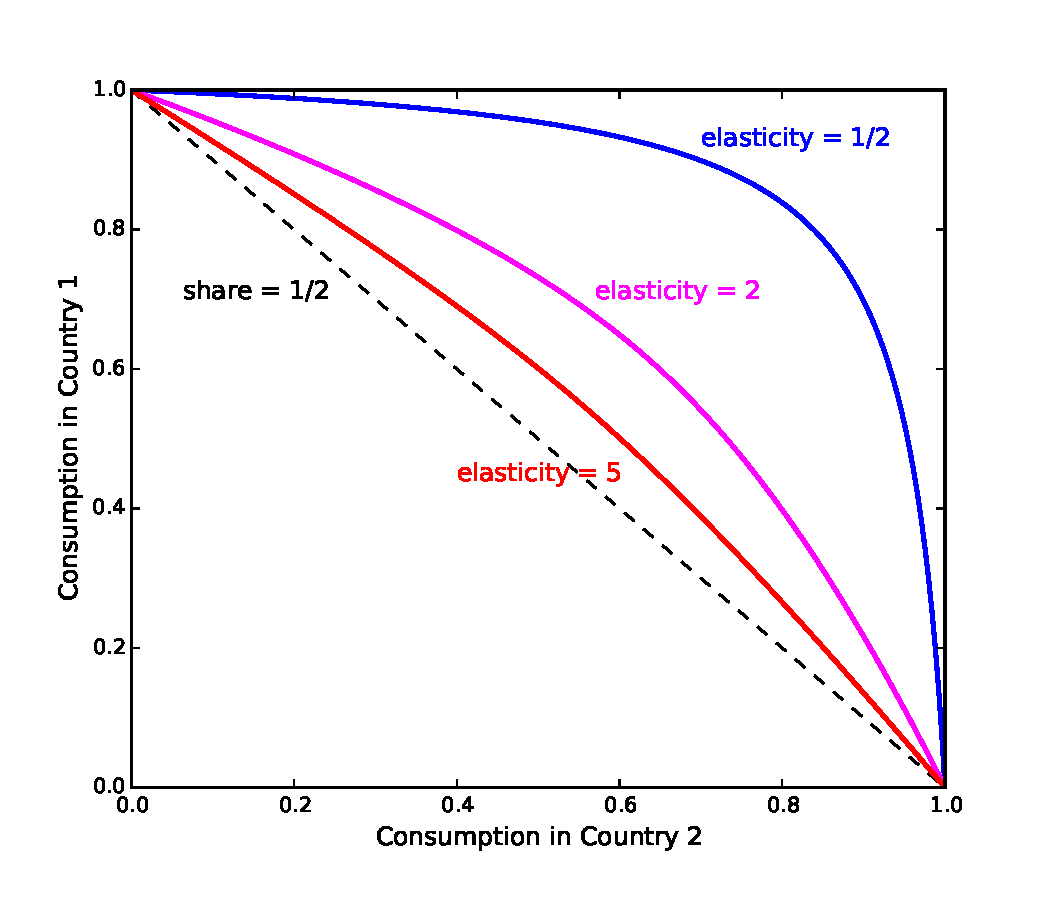
\includegraphics[width=\textwidth]{images/BCFL/final-goods-frontier.pdf}
\label{fig:consumption-frontier}
\end{figure}


% ****************************************************************************
\clearpage
\begin{figure}[htb]
\caption{Pareto and consumption frontiers.
The outer line is the consumption frontier with benchmark parameter values.
The inner line is the Pareto frontier:  the utility $J$ of agent 1 given
promised utility $U$ to agent 2.
In each case, the other state variables are $z_{1t} = z_{2t} = \wh{z}_t = 1$
and $v_t = v$.}

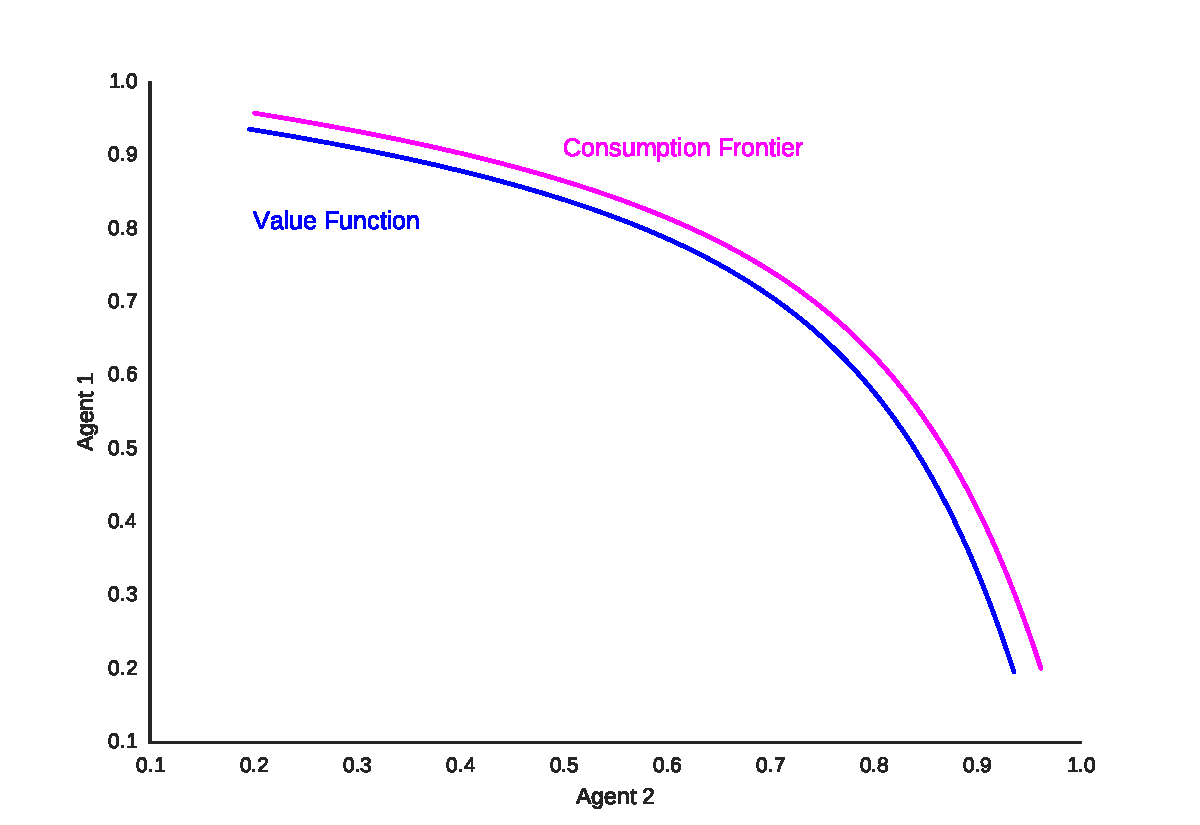
\includegraphics[width=\textwidth]{images/BCFL/frontiers_alpha9.pdf}
\label{fig:pareto-frontier}
\end{figure}


% ****************************************************************************
\clearpage
\begin{figure}[htb]
\caption{Dynamics of the additive and recursive Pareto weight.
The two lines represent simulations of models with additive ($\alpha = \rho = -1$)
and recursive ($\alpha = -9$, $\rho = -1 $) preferences.
The simulations use the same paths for exogenous state variables.
In each case, we plot $\log \lambda_t^*$ against time. }

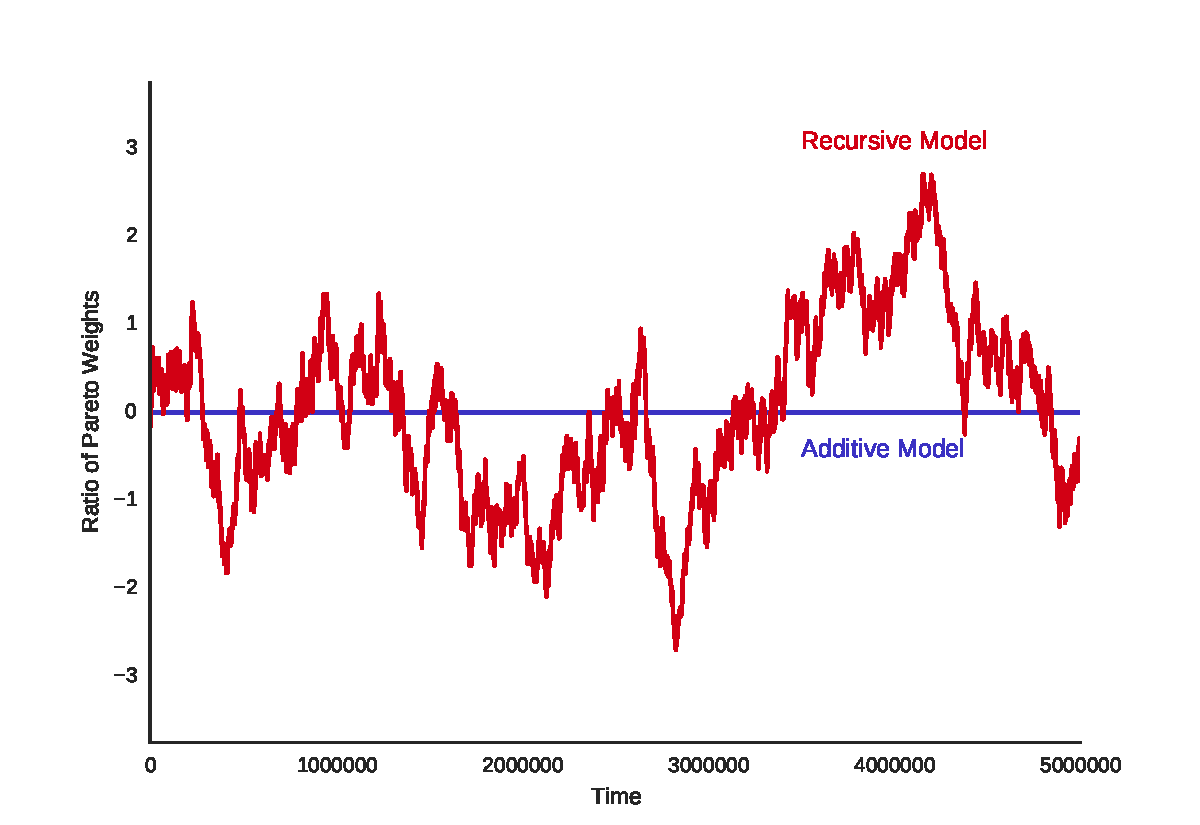
\includegraphics[width=\textwidth]{images/BCFL/paretoweightstability_alpha9.pdf}
\label{fig:exchange-pareto-weight-two}
\end{figure}


% ****************************************************************************
\clearpage
\begin{figure}[htb]
\caption{Risk aversion and expected changes in the Pareto weight.
The lines represent the expected change in $\log \lambda_t^*$, or $E_t[\log \lambda^*_{t+1}] - \log \lambda_t$,
with three values of risk aversion $1-\alpha$:
$2$ (additive), 10, and 50. }

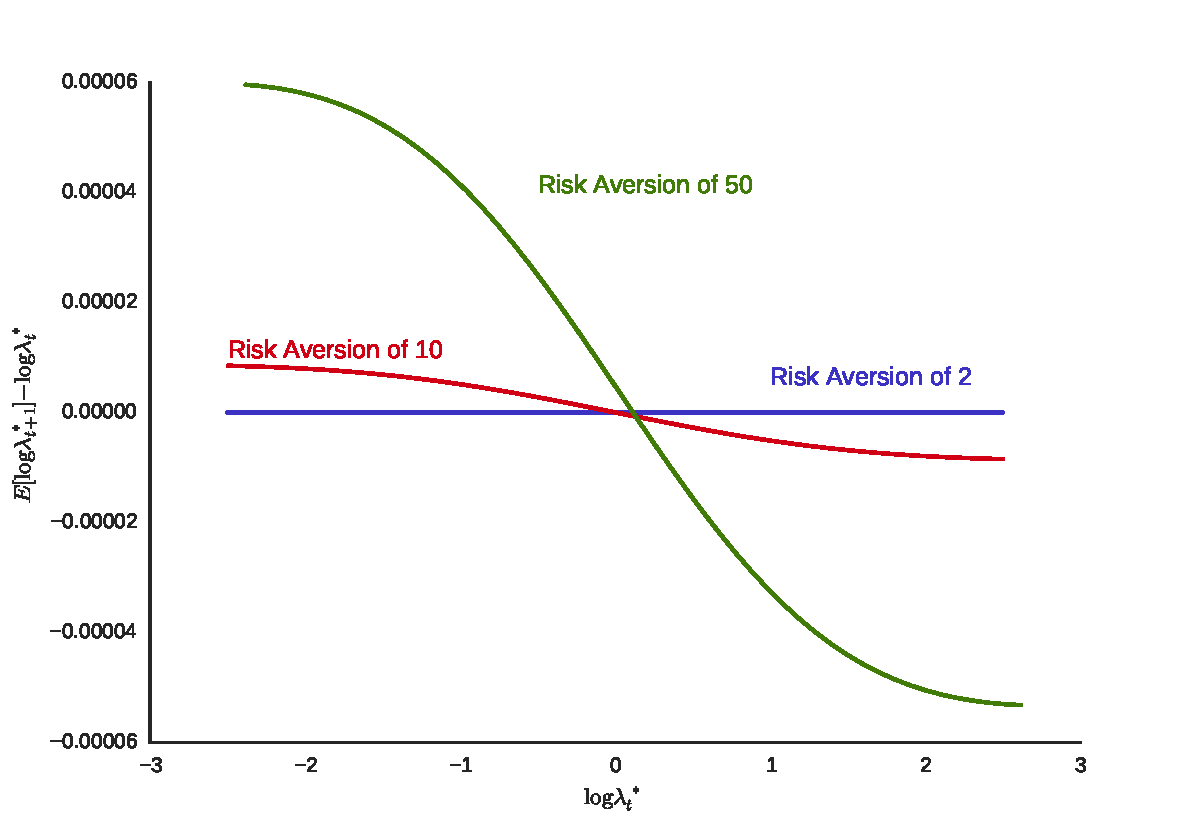
\includegraphics[width=\textwidth]{images/BCFL/policy_at_ss_one_axis.pdf}
\label{fig:change-pareto-weight-ra}
\end{figure}


% ****************************************************************************
\clearpage
\begin{figure}[htb]
\caption{Armington substitutability and expected changes in the Pareto weight.
The lines represent the expected change in $\log \lambda_t^*$, or $E_t[\log \lambda^*_{t+1}] - \log \lambda_t$,
with three values of the substitutability parameter $\sigma$ in the Armington aggregator.
The elasticities $1/(1-\sigma)$ are 2/3, 1, and 2. }

\bigskip
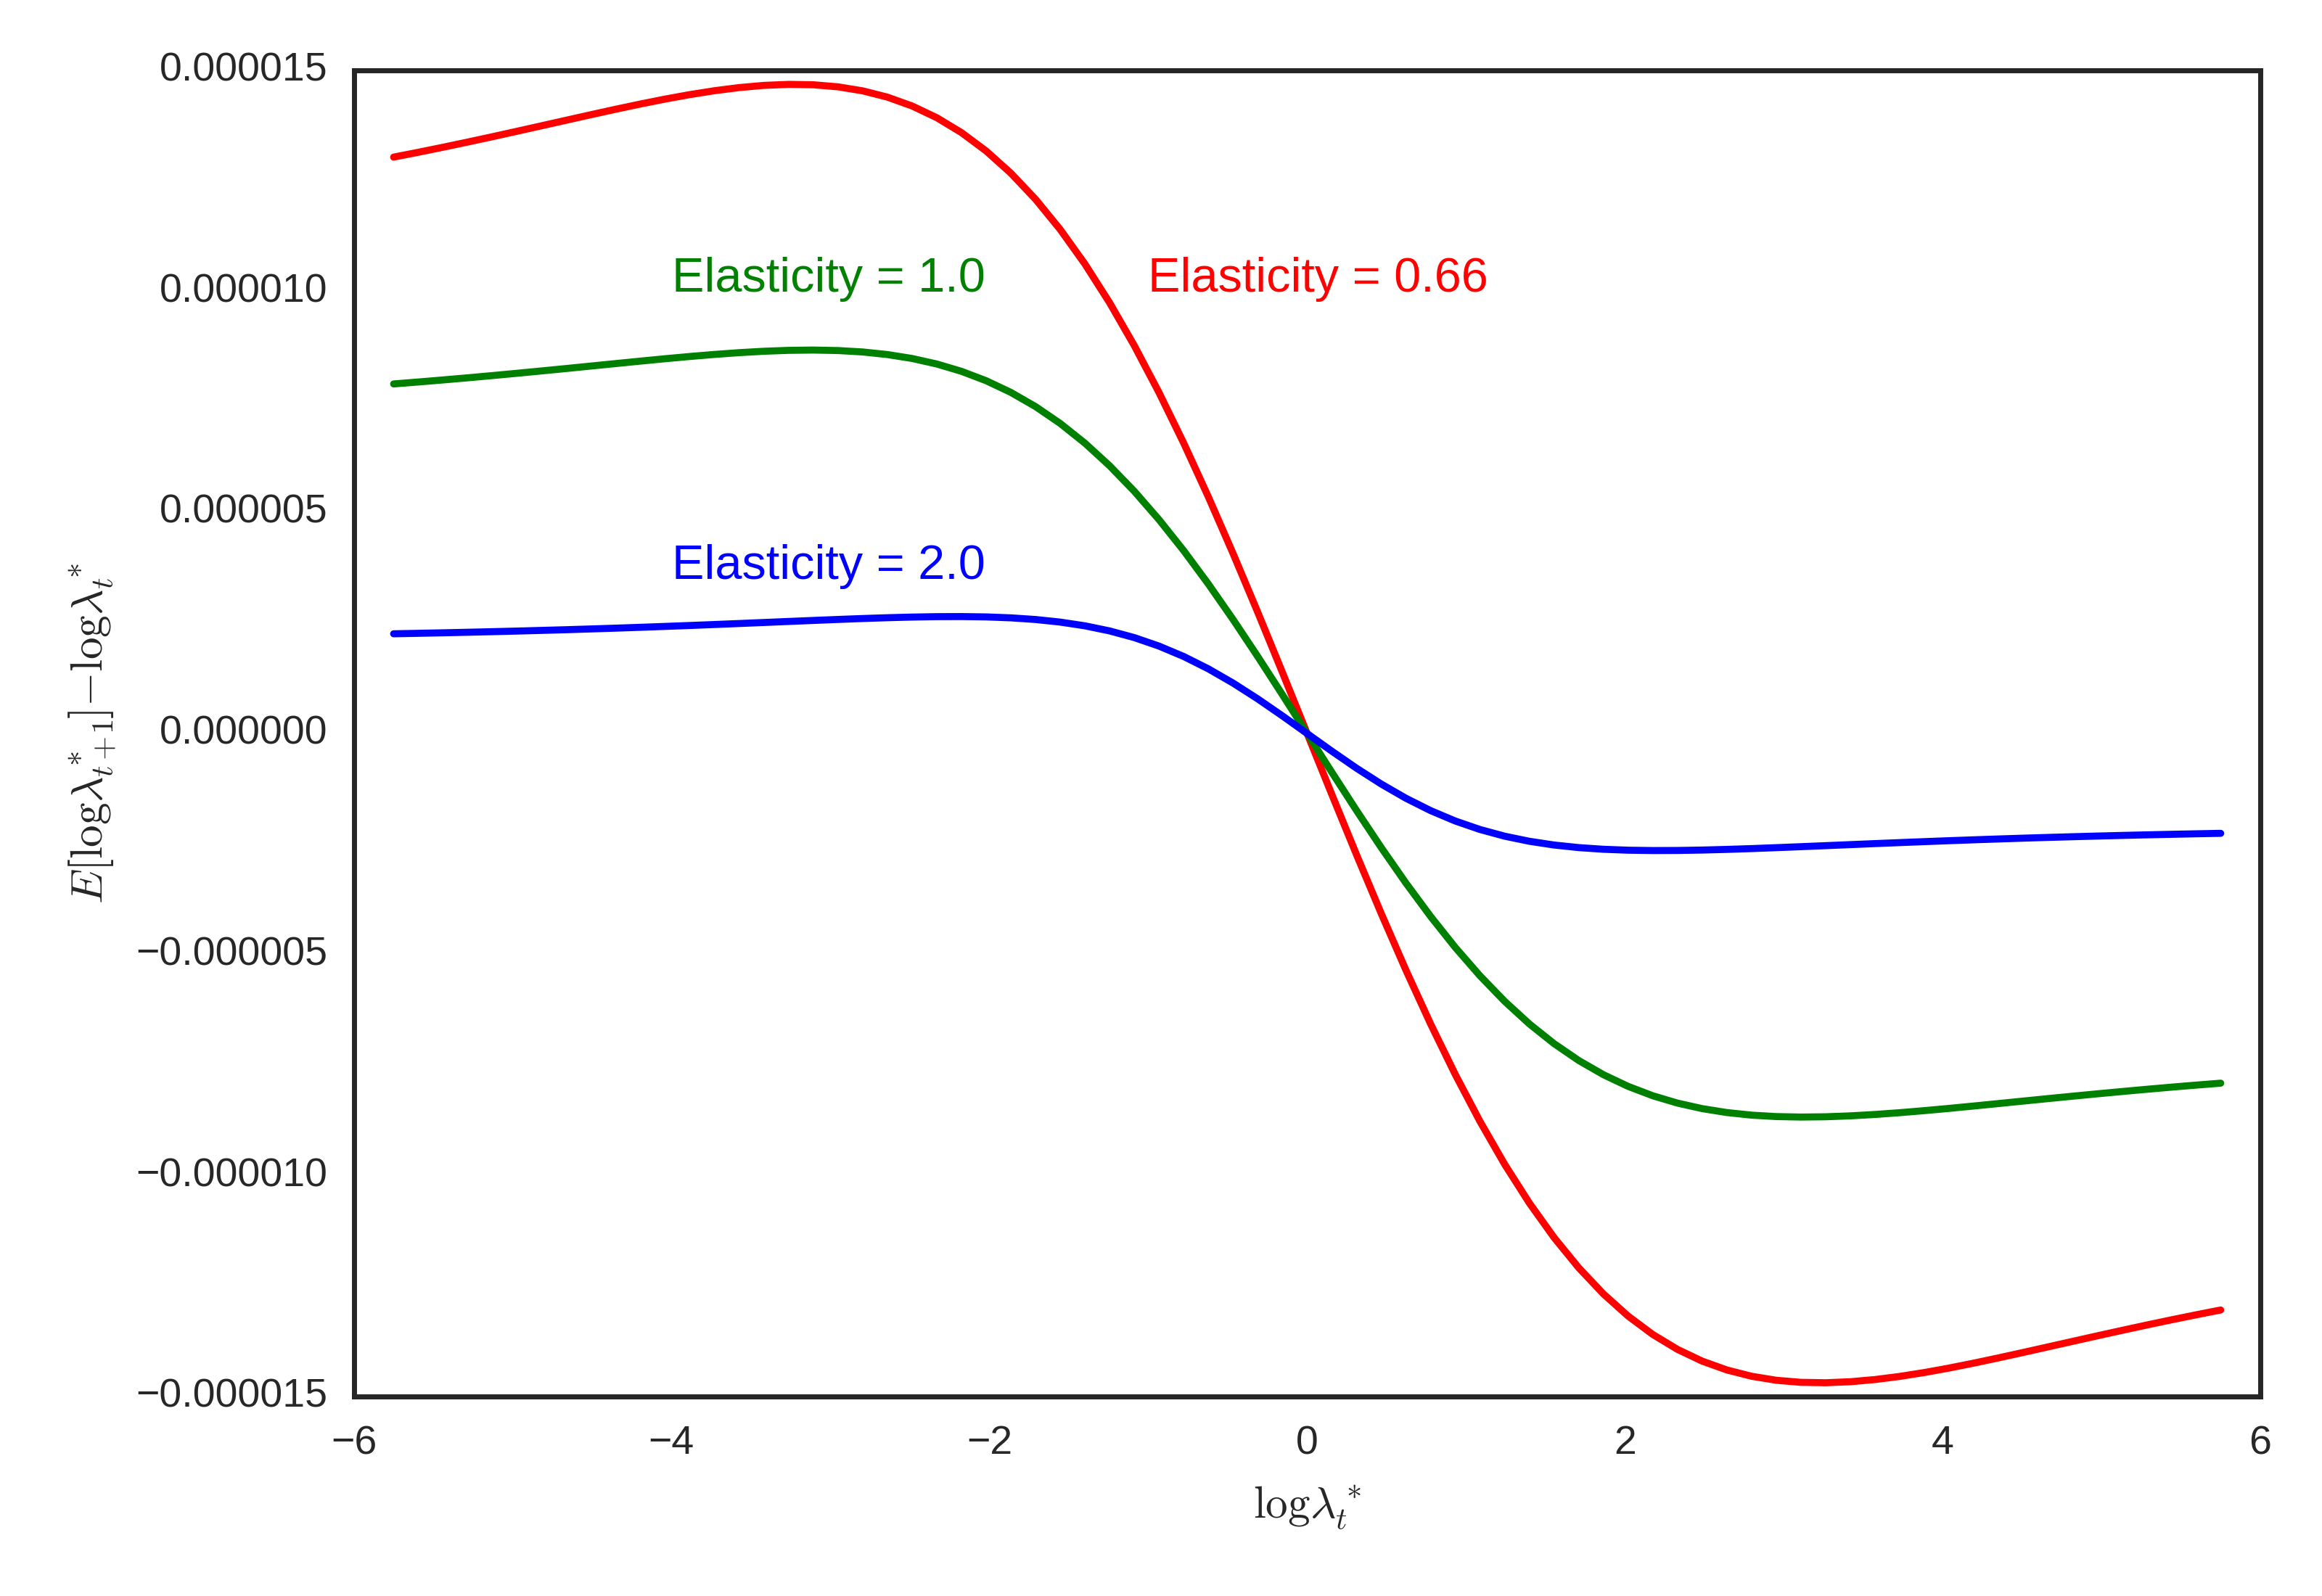
\includegraphics[width=\textwidth]{images/BCFL/Policies_Diff_Elast.png}
\label{fig:change-pareto-weight-arm}
\end{figure}

% ****************************************************************************
\clearpage
\begin{figure}[htb]
\caption{Intertemporal substitution and expected changes in the Pareto weight.
The lines represent the expected change in $\log \lambda_t^*$, or $E_t[\log \lambda^*_{t+1}] - \log \lambda_t$,
with three values of the substitutability parameter $\rho$ in the time aggregator:
$-1$, $-0.01$, and 1/3.
They correspond to intertemporal elasticities of substitution of 1/2, 0.99, and 3/2. }

\bigskip
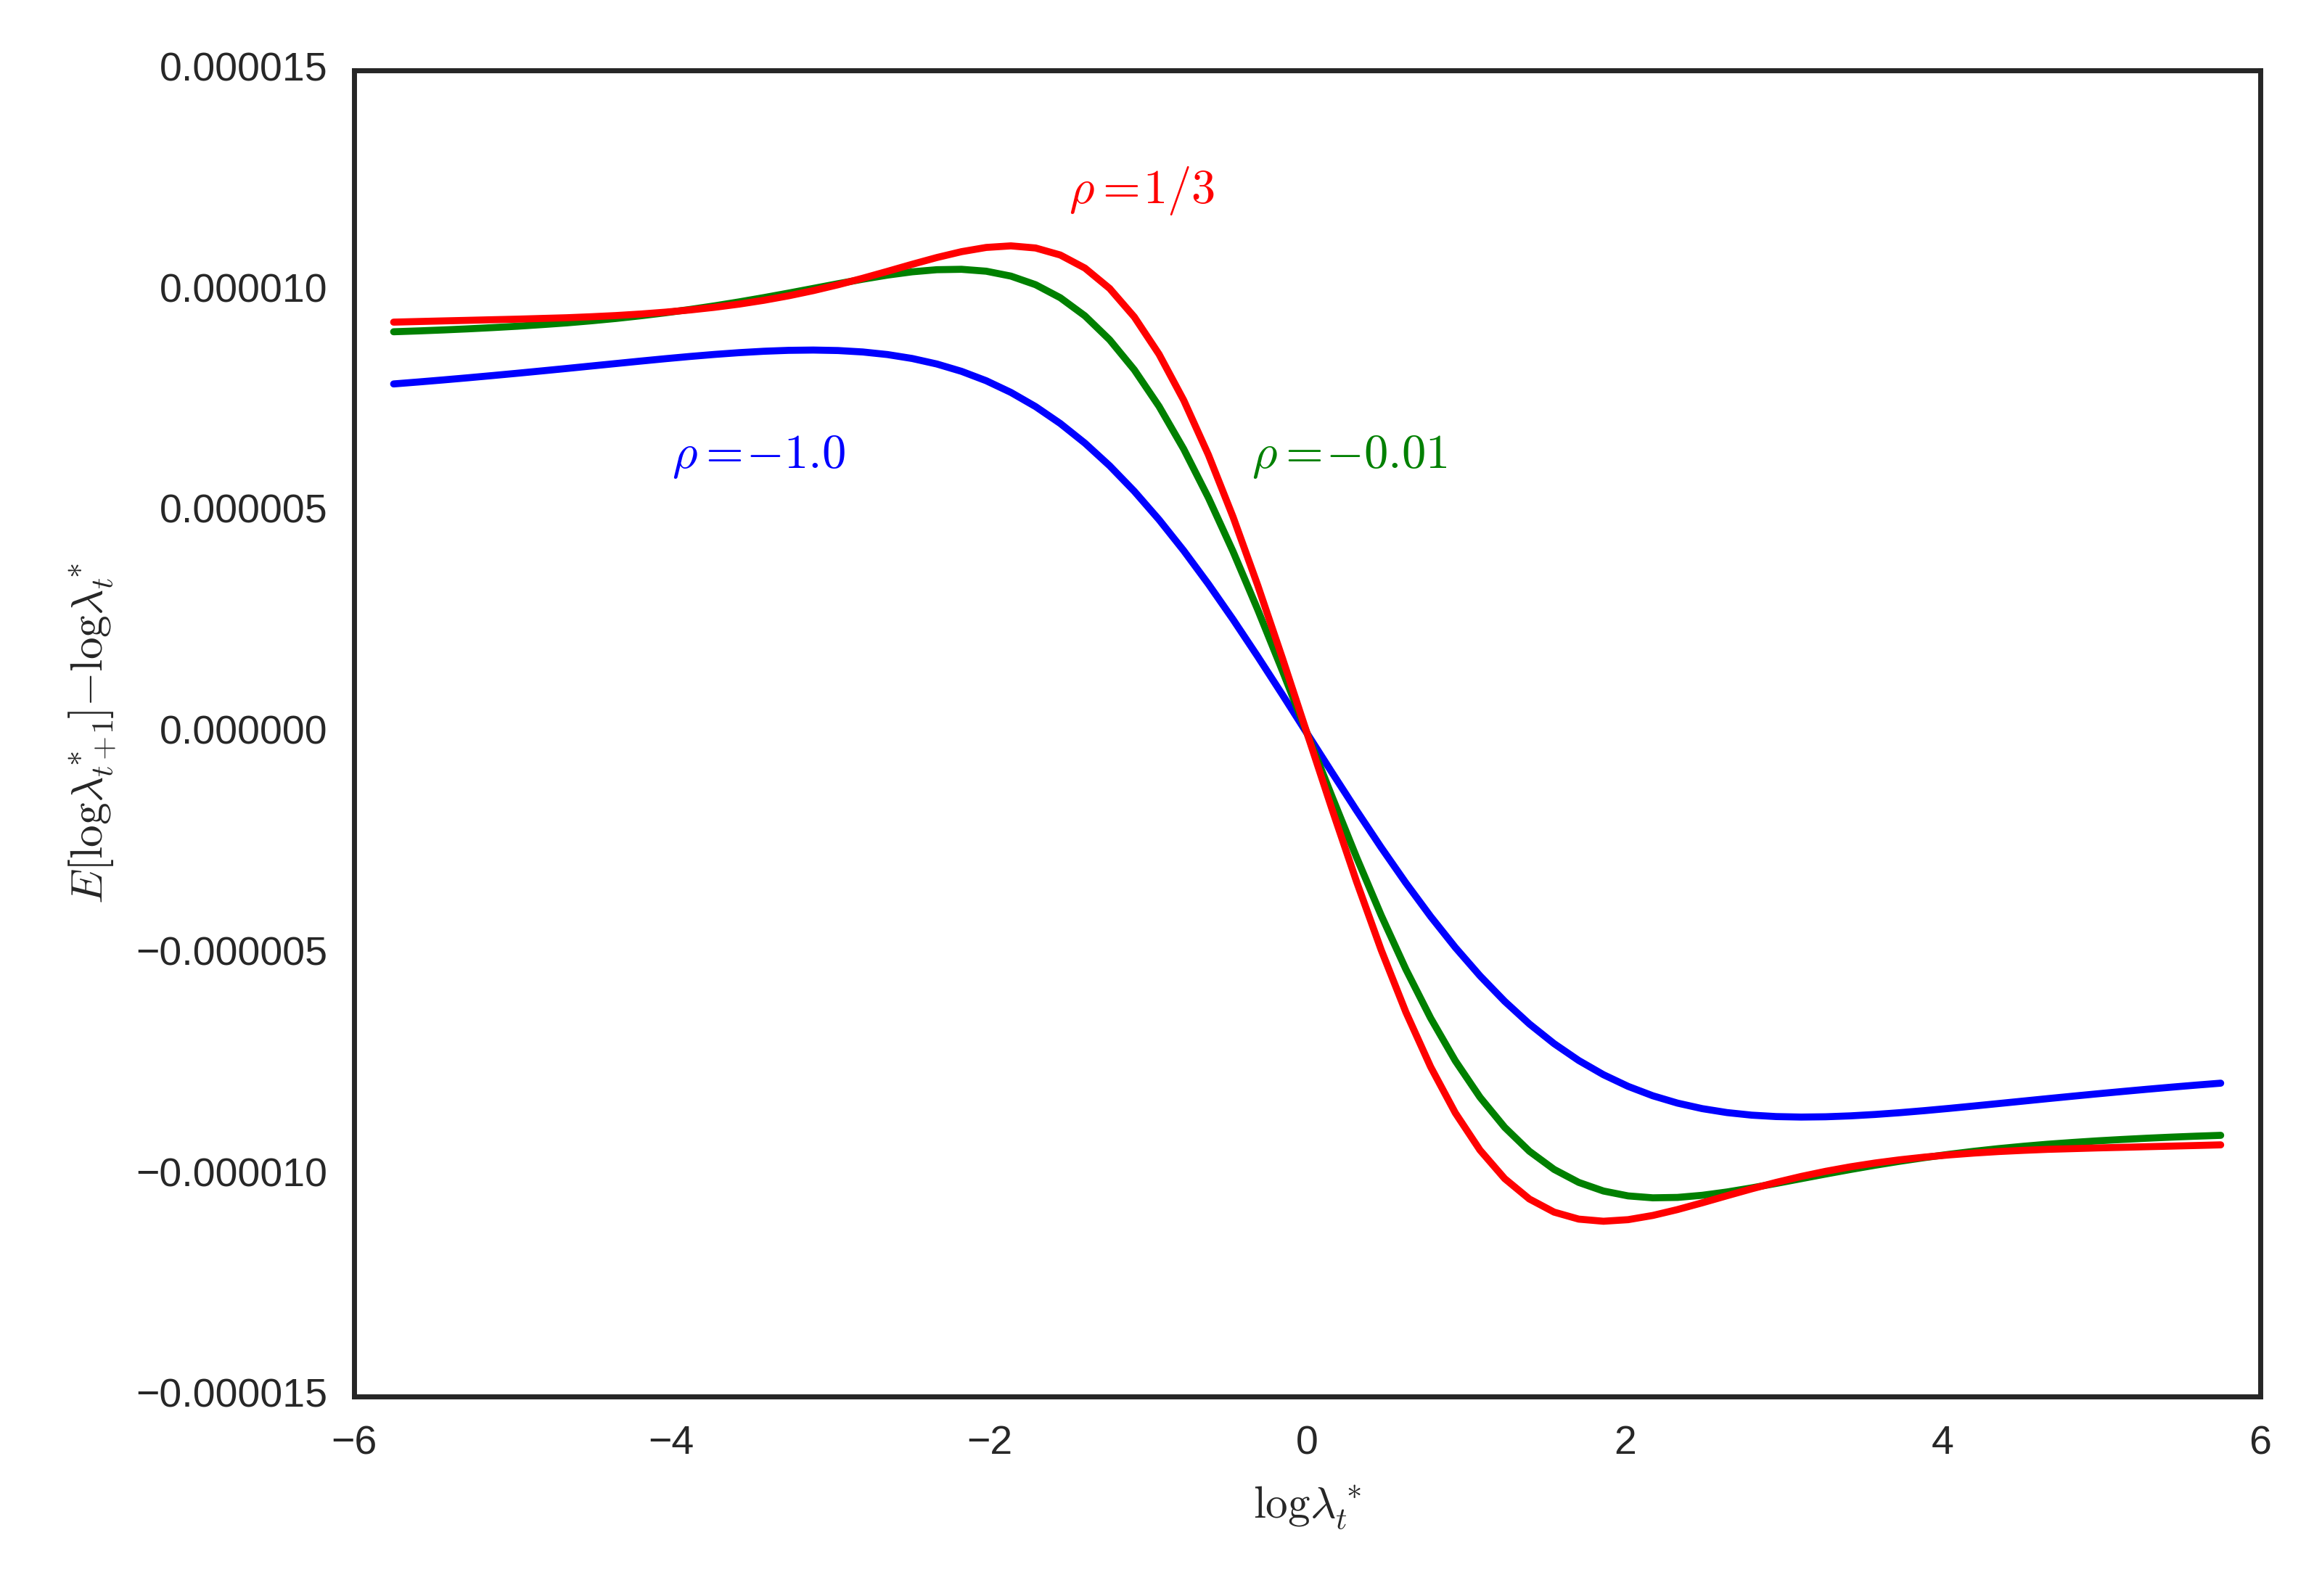
\includegraphics[width=\textwidth]{images/BCFL/Policies_Diff_rho.png}
\label{fig:change-pareto-weight-ies}
\end{figure}


% ****************************************************************************
\clearpage
\begin{figure}[htb]
\caption{Consumption and the real exchange rate.
The dots represent simulations of models with additive ($\alpha = \rho = -1$)
and recursive ($\alpha = -9$) preferences.
In each case, we plot  $\log e_t = \log (p_{2t}/p_{1t}) $ against $\log (c_{2t}/c_{1t}) $
for a simulation of the model. }

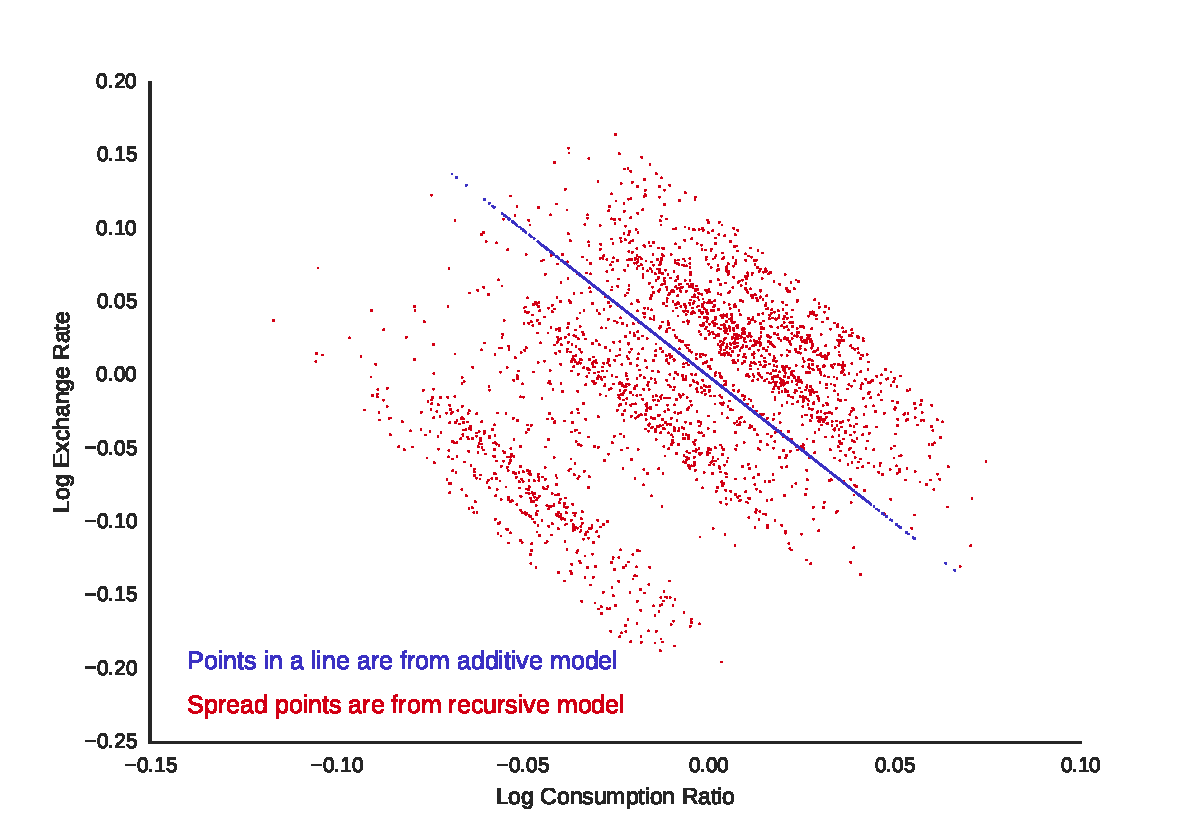
\includegraphics[width=\textwidth]{images/BCFL/con_v_fxr_alpha9.pdf}
\label{fig:exchange-cons-rer-two}
\end{figure}

%\end{document}
% ****************************************************************************
\clearpage
\begin{figure}[htb]
\caption{Dynamics of the real exchange rate.
The lines represent autocorrelation functions for the real exchange rate
($\log e_t$) in models with additive ($\alpha = \rho = -1$)
and recursive ($\alpha = -9$) preferences.}

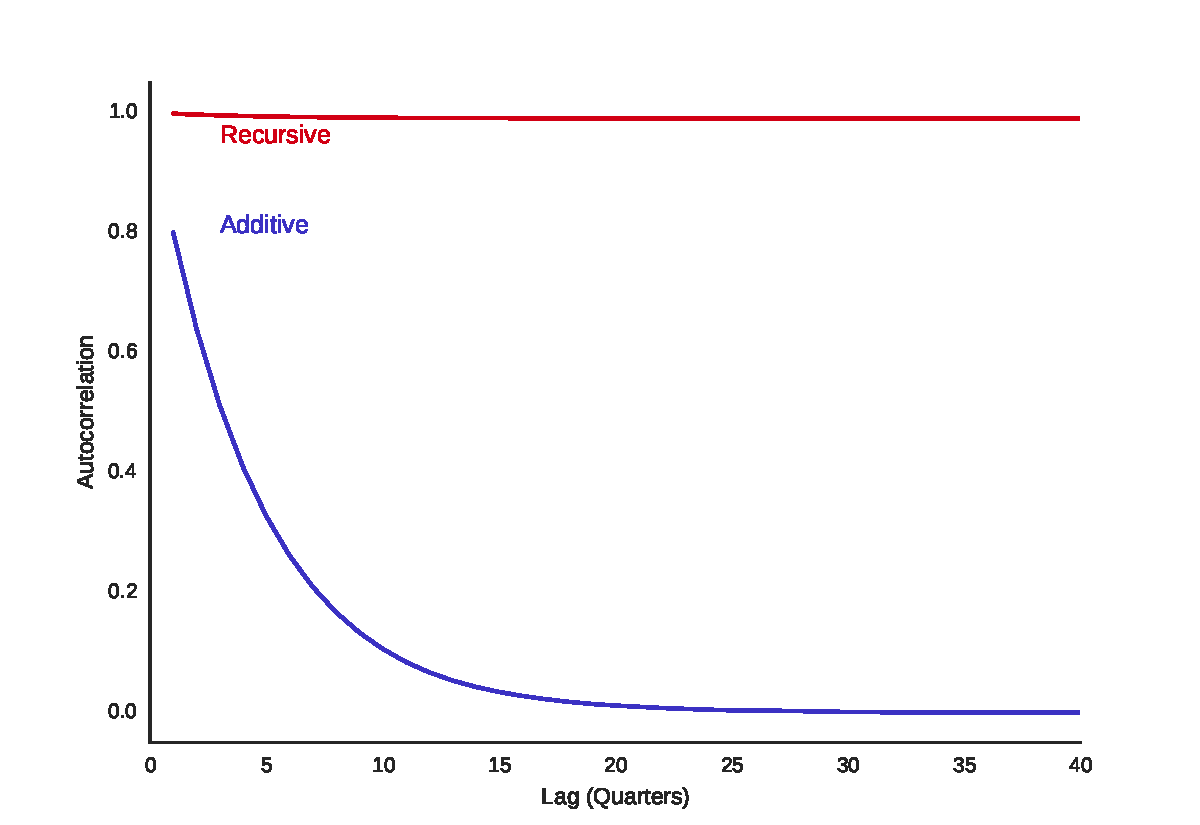
\includegraphics[width=\textwidth]{images/BCFL/acorr_fx_alpha1_9_one_axis.pdf}
\label{fig:rer-acfs}
\end{figure}

%\end{document}
% ****************************************************************************
\clearpage
\begin{figure}[htb]
\caption{Responses of variables
to an impulse in relative productivity\newline
$\log \wh{z}_t = (1/2) (\log z_{1t} - \log z_{2t}) $ in country 2.
The impulse takes place at date $t=1$.
Responses are reported as percent deviations from mean values.
}

\bigskip
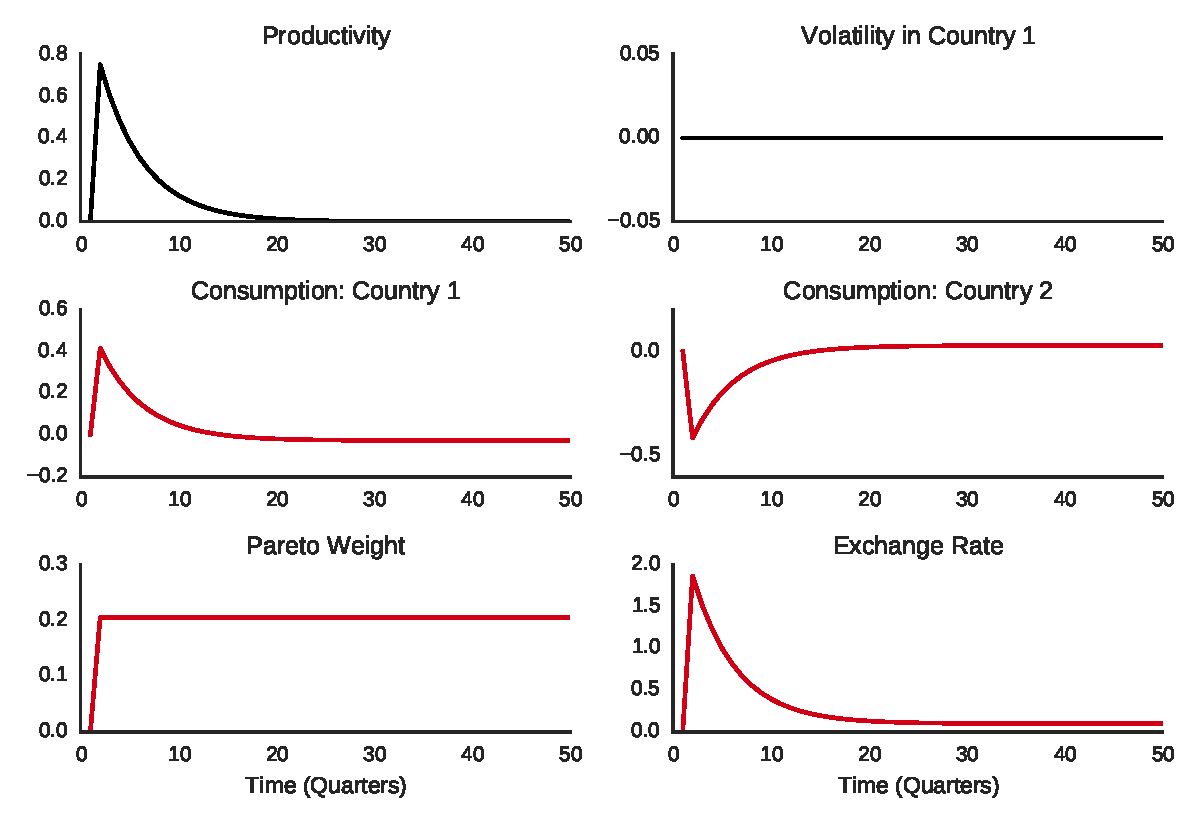
\includegraphics[width=\textwidth]{images/BCFL/irf_wrt_zhat_alpha9.pdf}
\label{fig:irf-zhat}
\end{figure}

%\end{document}
% ****************************************************************************
\clearpage
\begin{figure}[htb]
\caption{Responses of variables
to an impulse in volatility $v_t$.
The impulse takes place at date $t=1$.
Responses are reported as percent deviations from mean values.
}

\bigskip
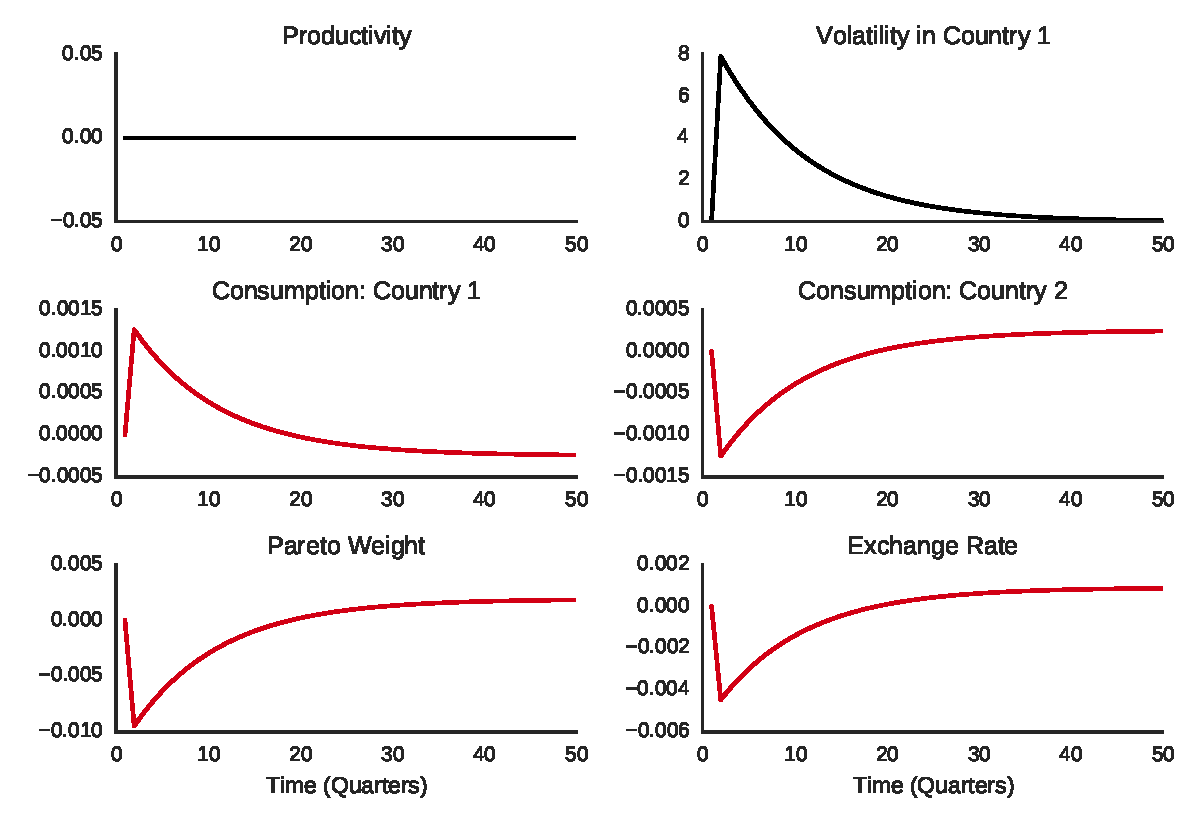
\includegraphics[width=\textwidth]{images/BCFL/irf_wrt_v_alpha9.pdf}
\label{fig:irf-v}
\end{figure}


\end{appendices}

\newpage

\clearpage

\backmatter

%%% BIBLIOGRAPHY

  \cftinserthook{toc}{BIB}
  \begin{OnehalfSpace}
    \bibliographystyle{ecta}
    \bibliography{combined}
  \end{OnehalfSpace}

\end{document}
